\chapter[PB-2a WHWP]{A warm HWP for PB-2a}
\label{ch:pb2a_whwp}

Building on the successes of its predecessor experiment POLARBEAR (PB-1), Simons Array (SA) employs an acrhomatic half-wave plate (AHWP) polarization modulator on each of its three telescopes. POLARBEAR-2a (PB-2) fields an ambient-temperature HWP---or a ``warm'' HWP (WHWP)---operating in front of the receiver cryostat vacuum window, while PB-2b and PB-2c employ a cryogenic HWP (CHWP) located inside the cryostat (see Chapter~\ref{sec:telescope_optics} for more details). In this chapter, we discuss the WHWP for POLARBEAR-2a (PB-2a), including its requirements, design, construction, and laboratory evaluation.

Before diving into the specifics of the WHWP instrument, we review the historical context surrounding the PB-2a experiment, which motivates several of the WHWP's design trajectories. Before SA came to be in 2015, POLARBEAR-2 (prior to the ``a/b/c'' labels) was a fully-funded, joint venture between researchers at the KEK high energy research organization in Japan\footnote{KEK CMB group: https://www2.kek.jp/proffice/archives/intra-e/feature/2009/CMB.html} and researchers at UC Berkeley. The PB-2 receiver cryostat was designed and built in Japan, the PB-2 detectors and readout were developed and fabricated in Berkeley, and the telescope, nearly identical to that of PB-1, was constructed commercially in Italy. The principle of the PB-2 design were to leverage PB-1's effective technologies---such as the Huan Tran Telescope, lenslet-coupled antennas, and frequency-domain multiplexing---to build another world-class instrument with via a concentrated set of hardware upgrades, and some of the most prominent upgrades to PB-2 over PB-1 were a dichroic receiver, a larger-diameter optics tube and focal plane to enable a larger field-of-view (FOV), and a higher-frequency readout system to facilitate a larger multiplexing factor.

The original PB-2 design included a continuously rotating HWP operating at 4~K located at the Lyot stop. However, deploying an AHWP deep within the cryostat proved to be an enormous technical challenge, and as PB-2's deployment neared, it became clear that the HWP subsystem needed to be descoped. In 2014, PB-2 moved its AHWP from the Lyot stop to outside of the cryostat, dramatically reducing the technological challenges surrounding the HWP's development and construction. Therefore, the presented WHWP research was conducted at UC Berkeley between 2014 and 2016 in parallel with the commissioning of the PB-2's detectors, readout, and optics tube. Shortly following the PB-2 HWP descope, SA was born, PB-2 became PB-2a, and CHWPs for PB-2b and PB-2c became a pivotal development path, as discussed in Chapters~\ref{ch:chwp_design} and~\ref{ch:chwp_evaluation}.

The PB-2a WHWP is a three-stack Pancharatnam sapphire AHWP designed to modulate linear polarization for 90 and 150~GHz detectors simultaneously. It is located directly in front of the receiver cryostat's vacuum window and has a clear aperture diameter of 480~mm. In the following sections, we present the WHWP's requirements, optical and mechanical design, and evaluation in the laboratory. The presented system has deployed to Chile and is ready to operate following the commissioning of the PB-2a detectors and readout.

%%%%%%%%%%%%%%%%%%%%%%%%%%%%%%%%
%%%%%%%%%%%%%%%%%%%%%%%%%%%%%%%%
%%%%%%%%%%%%%%%%%%%%%%%%%%%%%%%%

\section{Requirements}
\label{sec:pb2a_whwp_requirements}

The PB-2a WHWP shares several design requirements with those of all SA HWPs, which are described in Section~\ref{sec:sa_hwp_requirements}, including a 2~Hz rotational velocity, $>$~95\% modulation efficiency, and an angle encoder noise of $\ll$~3~$\mathrm{\mu K / \sqrt{Hz}}$. However, there are several other requirements specific to the WHWP that we review in this section, including its aperture diameter, reflectivity, and emissivity.

%%%%%%%%%%%%%%%%%%%%%%%%%%%%%%%%
%%%%%%%%%%%%%%%%%%%%%%%%%%%%%%%%

\subsection{Clear aperture diameter}
\label{sec:pb2a_whwp_clear_aperture_diameter}

There are two possible locations for the WHWP within the PB-2a system, each of which is shown in Figure~\ref{fig:pb2a_whwp_aperture_size}. The first location is at prime focus between the primary and secondary mirrors as was done in PB-1. The advantage of the prime-focus location is the small clear aperture diameter\footnote{The clear aperture diameter descries a circle that is unobstructed by any non-optical components.} needed to admit the beam\footnote{The telescope's beam is defined to be the collection of reverse-time-sense rays from all detectors on the focal plane. See Figure~\ref{fig:pb2a_whwp_aperture_size:a} for a visual representation.}, which in turn relaxes many aspects of the optical and mechanical designs. However, there are several disadvantages to operating the CHWP between the telescope's mirrors. First, the prime focus is the focus\footnote{The telecentric FOV of the primary mirror alone is small, and therefore the prime focus is only a true focus pixels for a small subset of detector pixels, as. Even so, the beam for all detectors at prime focus is tightly collimated relative to the rest of the imaging system.} of the primary mirror, and therefore each detector pixel illuminates a small fraction of a prime-focus HWP's surface, as shown in the left panel of Figure~\ref{fig:pb2a_whwp_aperture_size:b}. This optical configuration is prone to half-wave plate synchronous signals (HWPSSs) caused by position-dependent (and therefore rotation-angle-dependent) variations in the WHWP's optical assembly, such as defects in the anti-reflection (AR) coating or in the sapphire stack. Second, a prime-focus HWP is far from the cryostat, making it particularly exposed to 300~K scattering and stray reflections, which in turn increase parasitic optical power on the detectors. In addition, while much of this scattered radiation (in the time-reverse sense) is expected to ``land'' on the telescope's comoving\footnote{Comoving refers to any structure that is attached to the telescope such that it moves with telescope boresight.} baffling, some will ``escape'' the telescope structure and ``land'' on the ground. This \important{ground pickup} introduces azimuth- and elevation-dependent signals in the detector data that, while removable, degrade signal to noise, especially on large angular scales. Third, placing an optical element between the mirrors of a crossed Dragone configuration breaks the \important{Mizuguchi-Dragonne (MD) condition}, which is the secondary mirror's ability to correct cross polarization induced by the primary. This \important{MD breaking} was studied in detail for the PB-1 system and is expected to be larger in PB-2a due to a larger field of view and the AHWP's frequency-dependent angle.

\begin{figure}[!t]
    \centering
    \subfloat[\label{fig:pb2a_whwp_aperture_size:a}]{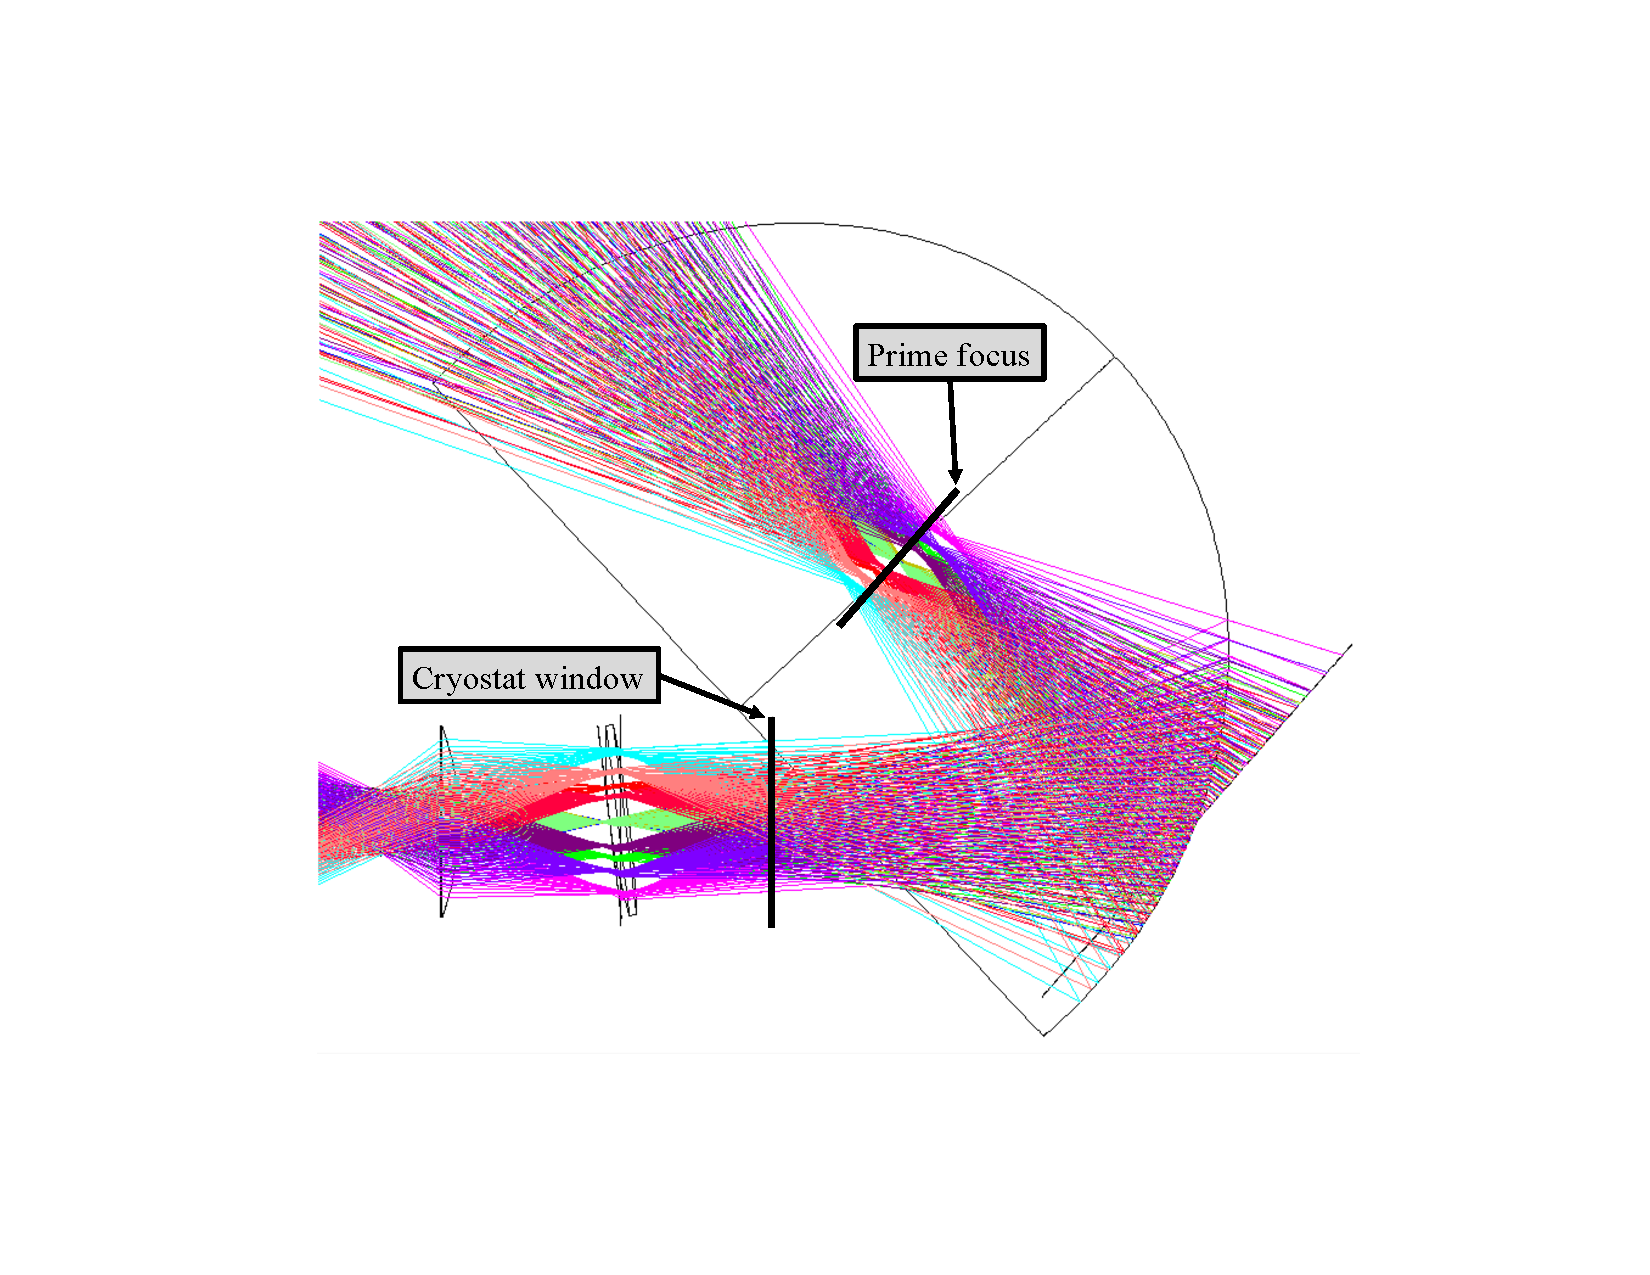
\includegraphics[width=0.9\linewidth, trim=2.5cm 5cm 2.5cm 5cm, clip]{PB2aWHWP/Figures/pb2a_whwp_ray_trace.pdf}}
    \hfill
    \subfloat[\label{fig:pb2a_whwp_aperture_size:b}]{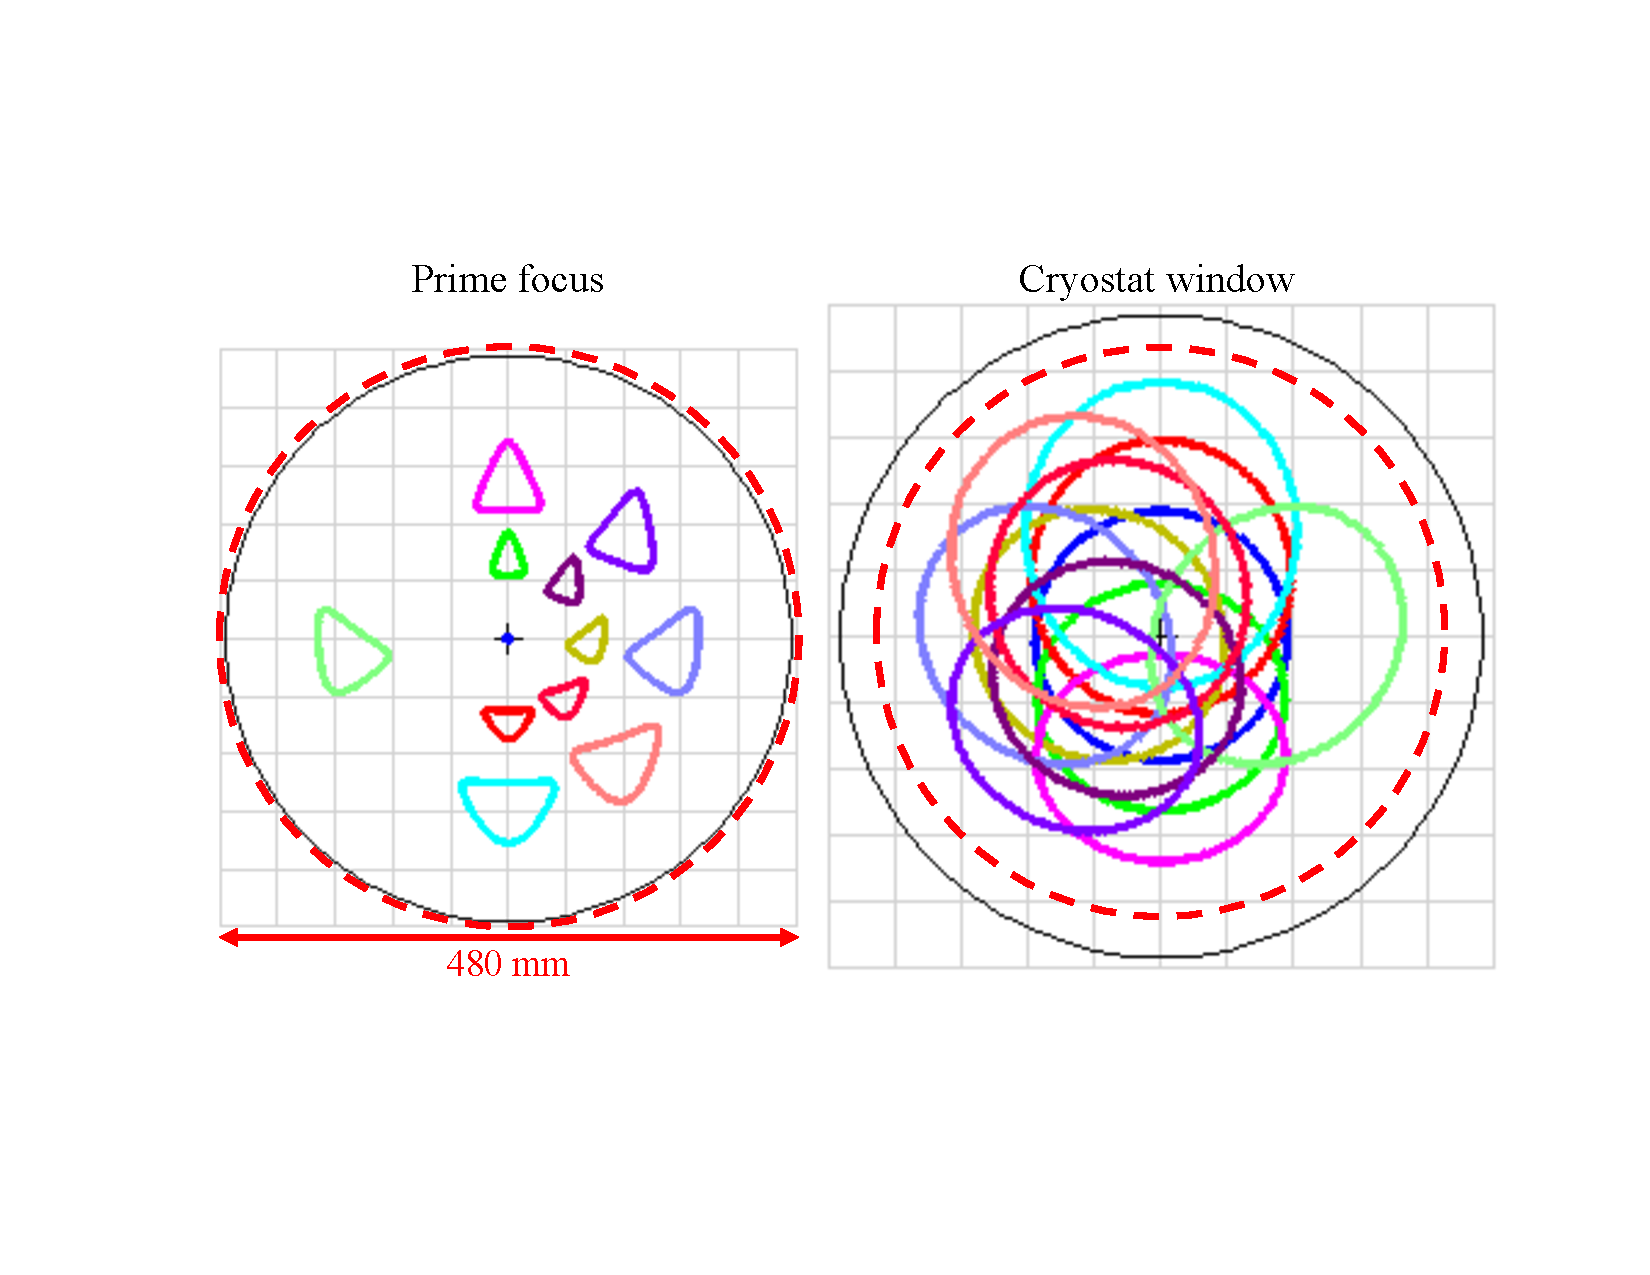
\includegraphics[width=0.75\linewidth, trim=2.5cm 5cm 2.5cm 4.2cm, clip]{PB2aWHWP/Figures/pb2a_whwp_aperture_size.pdf}}
    \caption[PB-2a ray trace simulation and the resulting WHWP clear aperture diameter requirement.]{PB-2a ray trace simulation and the resulting WHWP clear aperture diameter requirement. Figure~\ref{fig:pb2a_whwp_aperture_size:a} is a Zemax ray trace simulation of the PB-2a optical system including the telescope mirrors and reimaging optics. Each color corresponds to a distinct pixel on the focal plane. Figure~\ref{fig:pb2a_whwp_aperture_size:b} shows the \important{ray footprint} at both the cryostat window and prime focus planes. The WHWP's 480~mm clear aperture diameter has a wider margin at prime focus, each pixel's illumination pattern is larger at the cryostat window, in turn reducing HWPSSs due to non-uniformities in the optical stack.}
    \label{fig:pb2a_whwp_aperture_size}
\end{figure}

For these reasons, among others, the PB-2a WHWP is located at the second possible location, directly in front of the receiver cryostat. While this location requires a larger clear aperture diameter, it has a few key advantages over the prime-focus location. First, it is broadly illuminated by each detector pixel, as shown in the right panel of Figure~\ref{fig:pb2a_whwp_aperture_size:b}. This wider illumination pattern better averages each detector's beam over any position-dependent WHWP defects, hence reducing HWPSSs amplitudes. Second, the the vacuum-window location is both close to the cryostat and deep within the telescope baffling. Therefore, reflections at the WHWP  are (in the time-reverse sense) much more likely to land on cold surfaces, hence reducing the optical load on the detectors. In addition, any light scattered by the WHWP is much more likely to terminate on the telescope's comoving baffling, suppressing ground-synchronous signals compared to those induced by a prime-focus HWP. Finally, an AHWP at the cryostat window does not break the MD condition and hence induces minimal cross polarization. Despite the advantages of this second location, pushing the WHWP to a larger clear aperture diameter introduces other optical and mechanical challenges, which we discuss in the following sections, but PB-2a found the benefits to outweigh the risks.

Given its location directly in front of the receiver cryostat's vacuum window, the WHWP's clear aperture requirement is determined by assessing the \important{ray footprint} at the WHWP aperture plane, which is shown in the right panel of Figure~\ref{fig:pb2a_whwp_aperture_size:b}. The diametrical extent of the rays across the focal plane is 430~mm, and in order to provide margin for diffraction effects and alignment tolerances, we set a clear aperture requirement of $\geq$~480~mm.

%%%%%%%%%%%%%%%%%%%%%%%%%%%%%%%%
%%%%%%%%%%%%%%%%%%%%%%%%%%%%%%%%

\subsection{Emissivity and reflectivity}
\label{sec:pb2a_whwp_emissivity_relfectivity_requirements}

The most impactful consequence of moving the PB-2a HWP from the 4~K stage to 300~K is the corresponding increase in mm-wave power on the detectors. As discussed in Chapter~\ref{ch:cmb_instrument_sensitivity}, a CMB instrument's noise-equivalent temperature (NET) increases sharply \important{in-band optical power},\footnote{In-band optical power is defined to be the optical power within the detectors' observation bands, which for PB-2a are centered at 90 and 150~GHz and have bandwidths of $\sim$~30 and~$\sim$~40~GHz, respectively.} and therefore controlling WHWP thermal emission is central to mitigating sensitivity degradation. Along a similar vein, low reflectivity is central to the WHWP's success, not only because reflecting CMB photons decreases signal-to-noise but also because reflections from the WHWP surface are susceptible to landing on 300~K surfaces,\footnote{In contrast, ``warm reflections'' are less of an issue for cryogenic optics, which are deep within the cryostat and therefore are much more likely to reflect to cold surfaces, which in turn reduces the in-band optical load.} which in turn can dramatically increase in-band optical loading. While emissivity and reflectivity are largely decoupled physical effects, we discuss them together because the AR coating optimization, which is presented in Section~\ref{sec:pb2a_whwp_ar_coating}, considers trade-offs between the two.

\begin{figure}[!t]
    \centering
    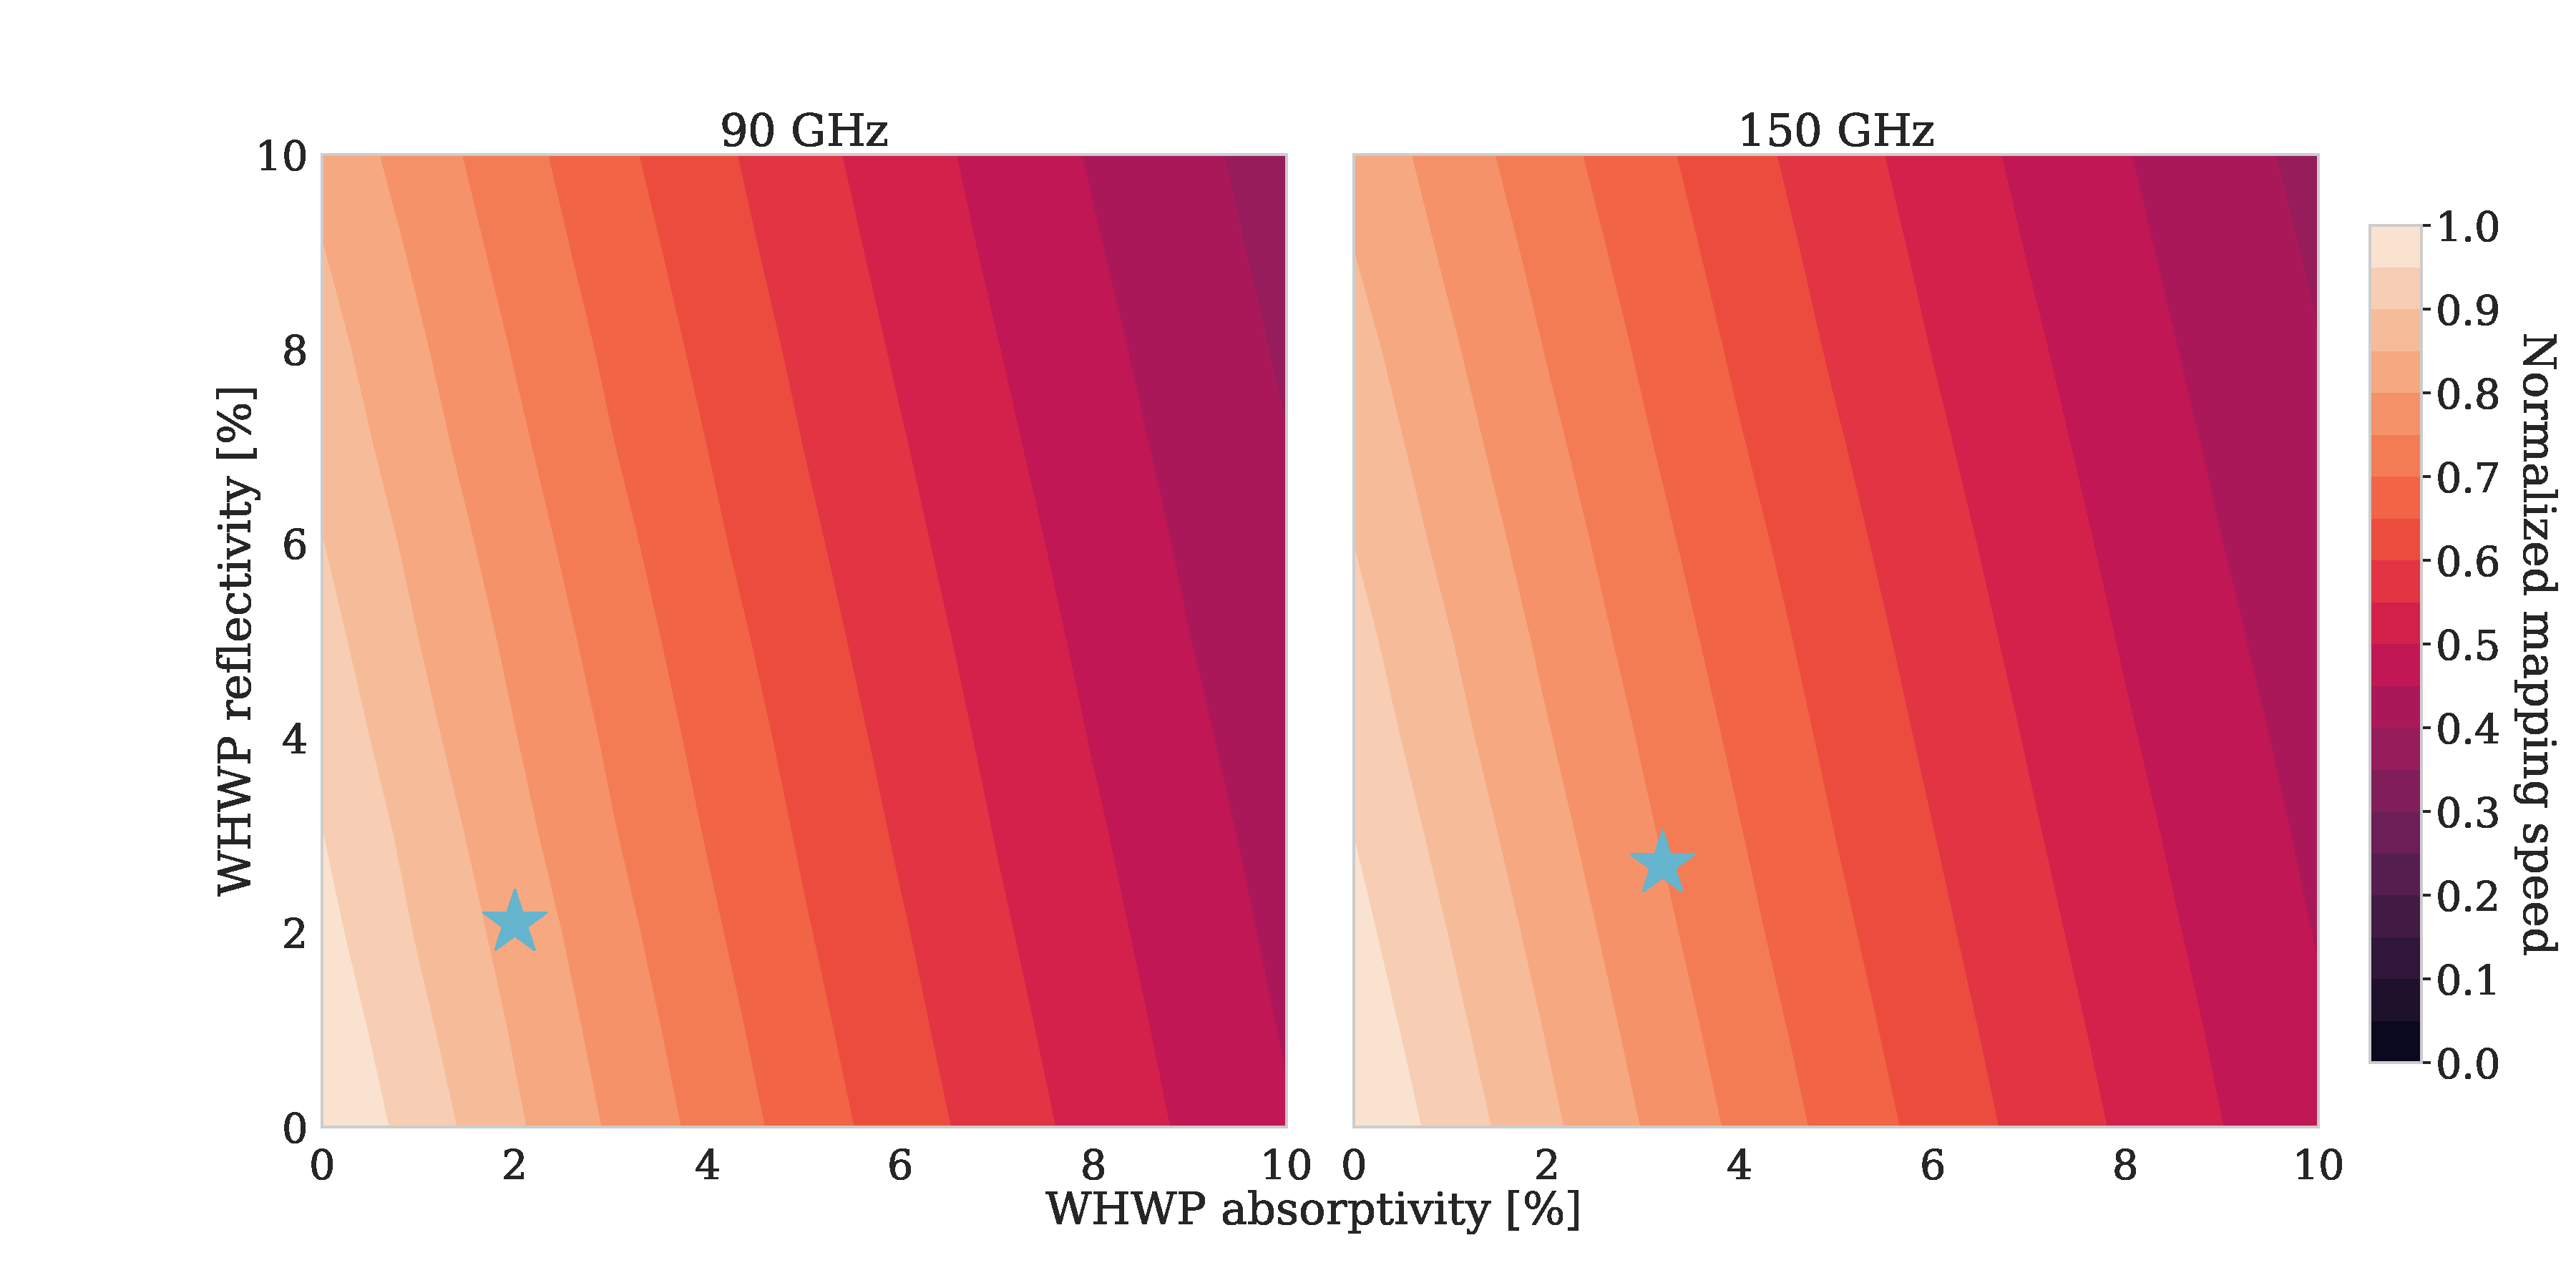
\includegraphics[width=\linewidth, trim=3cm 1cm 0cm 2.5cm, clip]{PB2aWHWP/Figures/pb2a_whwp_absorption_reflection_mappingSpeed.pdf}
    \caption[Impact of WHWP emissivity and reflectivity on PB-2a mapping speed.]{The impact of WHWP emissivity and reflectivity on PB-2a mapping speed in the 90 and 150~GHz bands using the measured optical properties shown in the table of Figure~\ref{fig:pb2a_whwp_bandpass}. The impact of emissivity is much stronger than that of reflectivity, which drives the AR coating design. While 150~GHz absorption tends to be generally larger than that at 90~GHz, the impact of emissivity itself is similar between the bands.}
    \label{fig:pb2a_whwp_emissivity_reflectivity_mappingSpeed}
\end{figure}

Figure~\ref{fig:pb2a_whwp_emissivity_reflectivity_mappingSpeed} shows PB-2a mapping speed (see Section~\ref{sec:N_ell_mapping_speed}) vs. WHWP emissivity and reflectivity. As demonstrated by the contour's orientation, instrument sensitivity depends more strongly on emissivity than on reflectivity, especially in the 150~GHz band, and for this reason, the PB-2a WHWP's AR coating is designed to minimize emissivity more aggressively than reflectivity.

%%%%%%%%%%%%%%%%%%%%%%%%%%%%%%%%
%%%%%%%%%%%%%%%%%%%%%%%%%%%%%%%%
%%%%%%%%%%%%%%%%%%%%%%%%%%%%%%%%

\section{Optical design}
\label{sec:pb2a_whwp_optical_design}

The PB-2a WHWP's \important{optical stack} is designed for high linear polarization modulation efficiency, low emissivity, and low reflectivity. It consists of three 512~mm-diameter, 3.75~mm-thick, $\alpha$-cut\footnote{An $\alpha$-cut sapphire plate's ordinary axis is normal to its surface such that normally incident light experiences optical birefringence. Another common orientation is c-cut sapphire, whose extraordinary axis is normal to its surface. This latter configuration is often used for sapphire windows, which aim to preserve incident polarization properties. Because there are two $\alpha$-axes and only one c-axis, it is substantially easier to grow large-diameter birefringent sapphire windows than non-birefringent.} sapphire plates fabricated via the advanced heat-exchange method at Guizhou Haotian Optoelectronics Technology (GHTOT)\footnote{GHTOT: http://www.ghtot.com/}. The plates are cut and ground with an $\alpha$-plane alignment of $\pm$ 2 degrees, a surface parallelism of $\pm$ 100 $\mu$m, and a surface roughness of 0.5 $\mu$m RMS, as determined at the manufacturer using a combination of micrometer and coordinate-measuring machine (CMM) measurements.

\begin{figure}[!t]
    \centering
    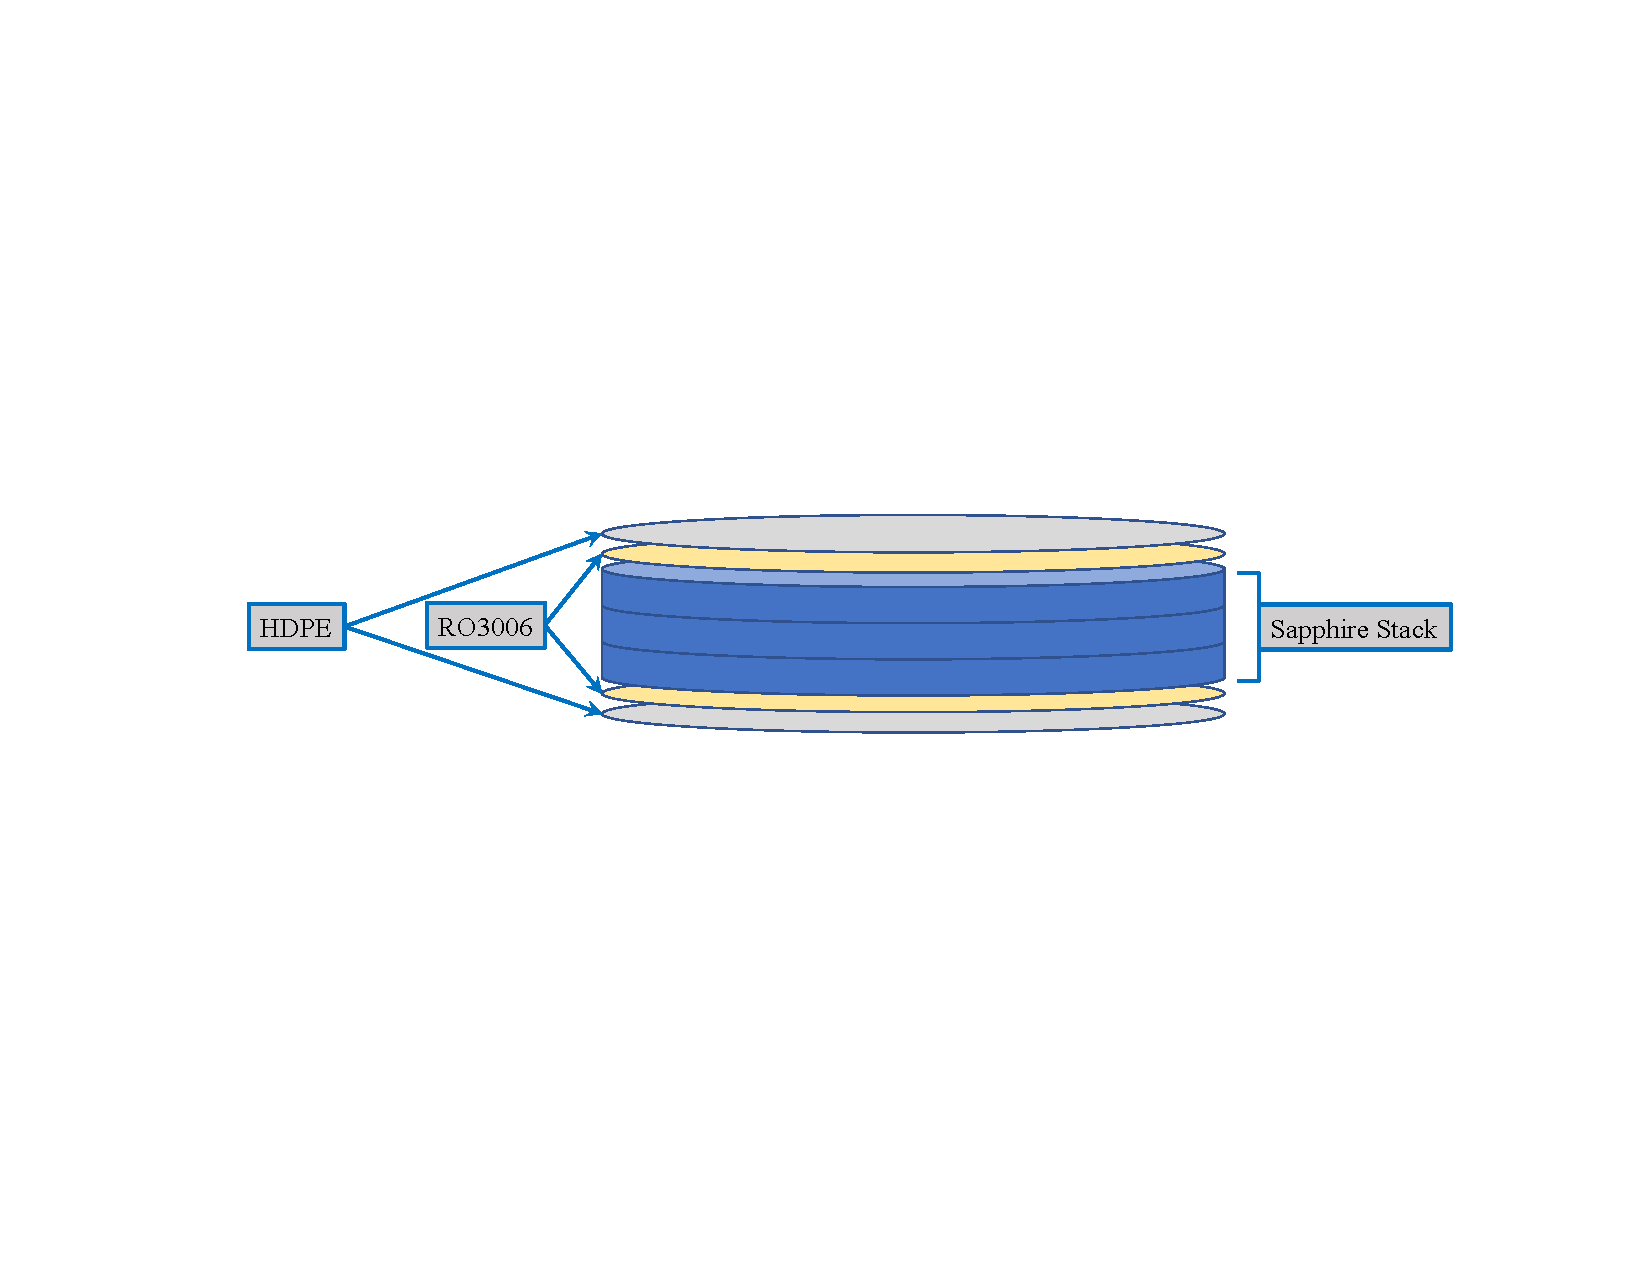
\includegraphics[width=\linewidth, trim=4cm 9cm 3cm 8cm, clip]{PB2aWHWP/Figures/pb2a_whwp_optical_stack_exploded.pdf}
    \caption{An exploded view of the WHWP optical stack, which is comprised of the Pancharatnam sapphire and a two-layer AR coating of HDPE and Rogers RT/Duroid RO3006.}
    \label{fig:pb2a_whwp_optical_stack_exploded}
\end{figure}

The AR coating comprises a top layer of 380~$\mu$m-thick of high-density polyethylene (HDPE)  from New Process Fibre (NPF)\footnote{NPF: http://www.newprocess.com/} and a bottom layer of 270~$\mu$m-thick of RT/Duroid RO3006\footnote{RO3006: https://rogerscorp.com/advanced-connectivity-solutions/ro3000-series-laminates/ \\ ro3006-laminates} circuit board laminate from Rogers Corporation. The AR layers are pressed onto the sapphire using ambient pressure, a technique that eliminates thermal emission associated with glue layers and avoids potential AR delamination during WHWP operation in the field. The table in Figure~\ref{fig:pb2a_whwp_mod_eff_spectrum} presents the measured parameters of the optical stack. The AR indexes were obtained using a Fourier Transform Spectrometer (FTS) (see Figure~\ref{fig:pb2a_whwp_bandpass}), the sapphire indexes using an FTS with aligned wiregrids on either side of the sample, and the loss tangents using the thermal emission apparatus described in Section~\ref{sec:pb2a_whwp_sapphire}. In the following subsections, we discuss the details of the WHWP's sapphire and AR coating.

%%%%%%%%%%%%%%%%%%%%%%%%%%%%%%%%
%%%%%%%%%%%%%%%%%%%%%%%%%%%%%%%%

\subsection{Sapphire}
\label{sec:pb2a_whwp_sapphire}

PB-2a selects sapphire as the birefringent substrate for its WHWP. Sapphire is single-crystal aluminum oxide $\mathrm{Al_{2}O_{3}}$ and has a large differential index $n_{\mathrm{e}} - n_{\mathrm{o}} \approx 0.35$ (see Equation~\ref{eq:hwp_ideal_thickness}) and a small loss tangent at $\sim$~100~GHz, making it ideal for CMB applications. The PB-2a sapphire is fabricated by GHTOT, which located in the Guizhou province in China. GHTOT produces among the largest sapphire in the world for an extraordinarily affordable price of $\sim$~5$\times$ less than U.S. competitors. GHTOT's sapphire boules\footnote{A ``boule'' is an industry term to describe the sapphire bulk that is removed from the furnace in which the sapphire is grown.} are grown using the \important{heat exchanger method (HEM)}  over the course of $\sim$weeks. After growth, the boule is inspected for ``smoke''---or microscopic defects such as bubbles or microcracks---the windows are cut from the boule using a wire saw, the crystal axis orientation is measured using x-ray diffractometry, and the windows are machined to their final shape via Blanchard grinding. One of the most challenging aspects of the PB-2a sapphire manufacturing process is the windows' high aspect ratio, which makes them particularly vulnerable to cracking during grinding. Therefore, GHTOT carefully approaches the final thickness with several passes of the grinding wheel, which both gives precise control of the overall part thickness and improves manufacturing yield.

\begin{figure}[!t]
    \centering
    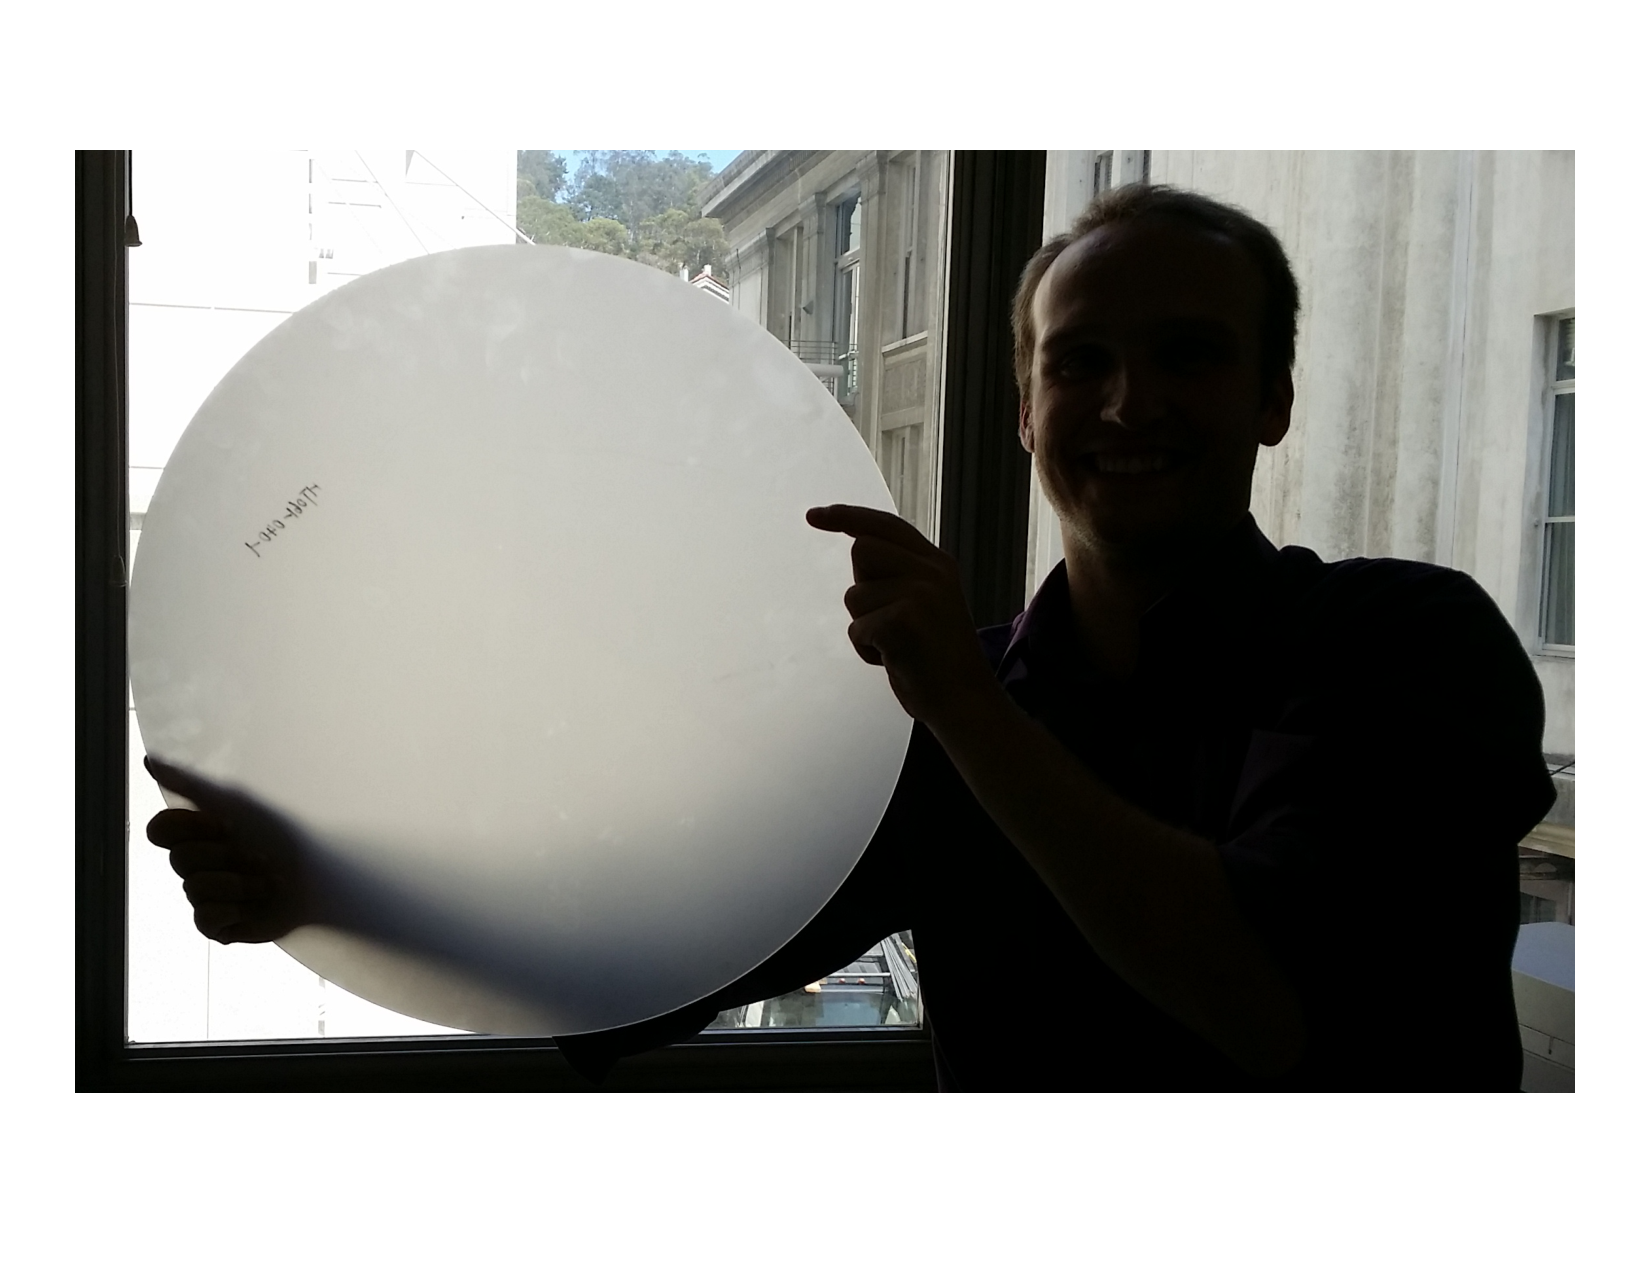
\includegraphics[width=0.7\linewidth, trim=0cm 3cm 3cm 3cm, clip]{PB2aWHWP/Figures/SapphirePicture.pdf}
    \caption[Photograph of GHTOT large diameter sapphire]{A photograph of the author holding the 512~mm-diameter GHTOT sapphire. The piece is ground to $\sim$ 0.1 $\mu$m surface roughness, giving it a frosty finish. Photo courtesy of Chris Raum (UC Berkeley).}
    \label{fig:sapphire_photo}
\end{figure}

Aside from cost and lead time, there are two primary considerations when assessing the usability of GHTOT sapphire for the PB-2a WHWP. The first consideration is the \important{optical diameter}, or the diameter which satisfies optical specifications. The PB-2a sapphire pieces are 512~mm in which allows the sapphire's fixture (see Section~\ref{sec:pb2a_whwp_mechanical_assembly}) to clamp $\Delta R = 5$~mm at the edge and allow for a $500$~mm clear aperture diameter, enabling the WHWP to meet its clearance specification of 480~mm with a comfortable margin for additional baffling and alignment tolerances. The second consideration is the sapphire's purity. In order to minimize its emissivity, the sapphire should be free of common contaminants, such as Titanium, Chromium, and Vanadium.\footnote{Pure sapphire is \textit{technically} called corundum, but the industry standard is to use ``sapphire'' as a blanket term for single-crystal aluminum oxide, no matter the purity.} Maintaining low impurity levels during sapphire growth is a challenging aspect of the manufacturing process and therefore was a fixation of PB-2a's sapphire selection process. GHTOT measures impurities in their sapphire boules using glow discharge mass spectroscopy (GDMS), and the bulk has $<$~1 part per million of all but tungsten, of which the growth crucible made. A photo of the GHTOT sapphire is shown in Figure~\ref{fig:sapphire_photo}, and the neutrality of the color is an excellent indicator of low impurity levels.

%%%%%%%%%%%%%%%%%%%%%%%%%%%%%%%%
%%%%%%%%%%%%%%%%%%%%%%%%%%%%%%%%

\subsection{Anti-reflection coating}
\label{sec:pb2a_whwp_ar_coating}

In order to meet PB-2a's performance targets in both the 90 and 150~GHz bands, the WHWP employs a dual-layer AR coating, as shown in Figure~\ref{fig:pb2a_whwp_optical_stack_exploded}. The chief objective of any AR coating is to minimize reflectivity, and the performance of PB-2a's AR coatings directly impacts the optical throughput of the telescope. For this reason, AR coatings are a an active research area within the scope of cutting-edge CMB instrumentation. Chapter~\ref{ch:sapphire_ar_coating} talks about AR coatings for cryogenic optics and presents a more comprehensive overview of techniques to minimize reflection, but in this section, we focus on the AR coating's construction and its impact on instrument sensitivity, as shown in Figure~\ref{fig:pb2a_whwp_emissivity_reflectivity_mappingSpeed}.

The PB-2a WHWP AR coating consists of two layers that slowly impedance match from the index of air $n_{\mathrm{air}} = 1$ to that of the sapphire $(n_{e} + n_{o}) / 2 = 3.21$. To leading order, the ideal AR indexes are (see Section~blah) $n_{\mathrm{bot}} = 2.31$ and $n_{\mathrm{top}} = 1.40$, and their ideal thicknesses are $\lambda_{\mathrm{c}} / (4 n)$, where $\lambda_{\mathrm{c}}$ is the AR band's central frequency. For PB-2a, $\nu_{\mathrm{c}} = c / \lambda_{\mathrm{c}} = 124$~GHz is directly between the two band centers. In addition to low reflectivity, it is critical that the AR layers be low emissivity to limit parasitic detector loading. According to Figure~\ref{fig:pb2a_whwp_emissivity_reflectivity_mappingSpeed}, the coating's emissivity is more important than its reflectivity, and therefore the PB-2a WHWP AR coating design employs materials with low mm-wave absorptivity.

The materials available for an ambient mm-wave AR coating are limited. Organic compounds, which are abundant in most commercially available products, absorb at $\sim$~100~GHz, and therefore our search is restricted to inorganic materials such as polyethylenes, fluoropolymers, and ceramics. The table in Figure~\ref{fig:pb2a_whwp_ar_layers} presents a catalog potential AR candidate materials measured using a 50~$\sim$~300~GHz FTS at UC Berkeley during WHWP development. Upon combining and simulating the achievable AR spectra for all permutations of the evaluated materials, we select RT/Duroid RO3006 circuit board laminate\footnote{The sheets are manufactured with copper cladding into which the desired circuit is etched. Therefore, our first step before using the sheets is to strip the copper, which we do using large baths of Ferric Chloride.} from Rogers Corporation as our bottom layer and high-density polyethylene (HDPE) as our top layer. RO3006 is a matrix of PTFE loaded with alumina grains which tune its dielectric constant, while the selected HDPE is manufactured by New Process Fibre (NPF) via a high-precision extrusion process. Both of these materials are low-loss in the PB-2a frequency range and have reproducible refractive indexes, making them suitable AR candidates.

\begin{figure}[!t]
    \centering
    \begin{tabu}{| c | c | c |}
	\hline
	Material & Measured $n$ & Measured $\tan \delta$ [$10^{-4}$] \\
	\hline
	\hline
	PTFE & $1.45 \pm 0.01$ & $3.0 \pm 1.5$\\
	\hline
	LDPE & $1.50 \pm 0.01$ & $10.2 \pm 2.4$ \\	
	\hline
	\textbf{HDPE} & $1.55 \pm 0.01$ & $0.5 \pm 1.0$ \\	
	\hline
	RT5880 & $1.56 \pm 0.01$ & $16.0 \pm 1.2$ \\ 
	\hline
	UHMWPE & $1.58 \pm 0.01$ & $2.6 \pm 6.2$ \\
	\hline
	RO3003 & $1.77 \pm 0.03$ & $21.1 \pm 0.8$ \\
	\hline
	\textbf{RO3006} & $2.52 \pm 0.01$ & $56.5 \pm 2.7$ \\
	\hline
	RT6006 & $2.86 \pm 0.02$ & $89.9 \pm 1.7$ \\
	\hline
	\end{tabu}
	\centering
    \subfloat[\label{fig:pb2a_whwp_ar_layers:a}]{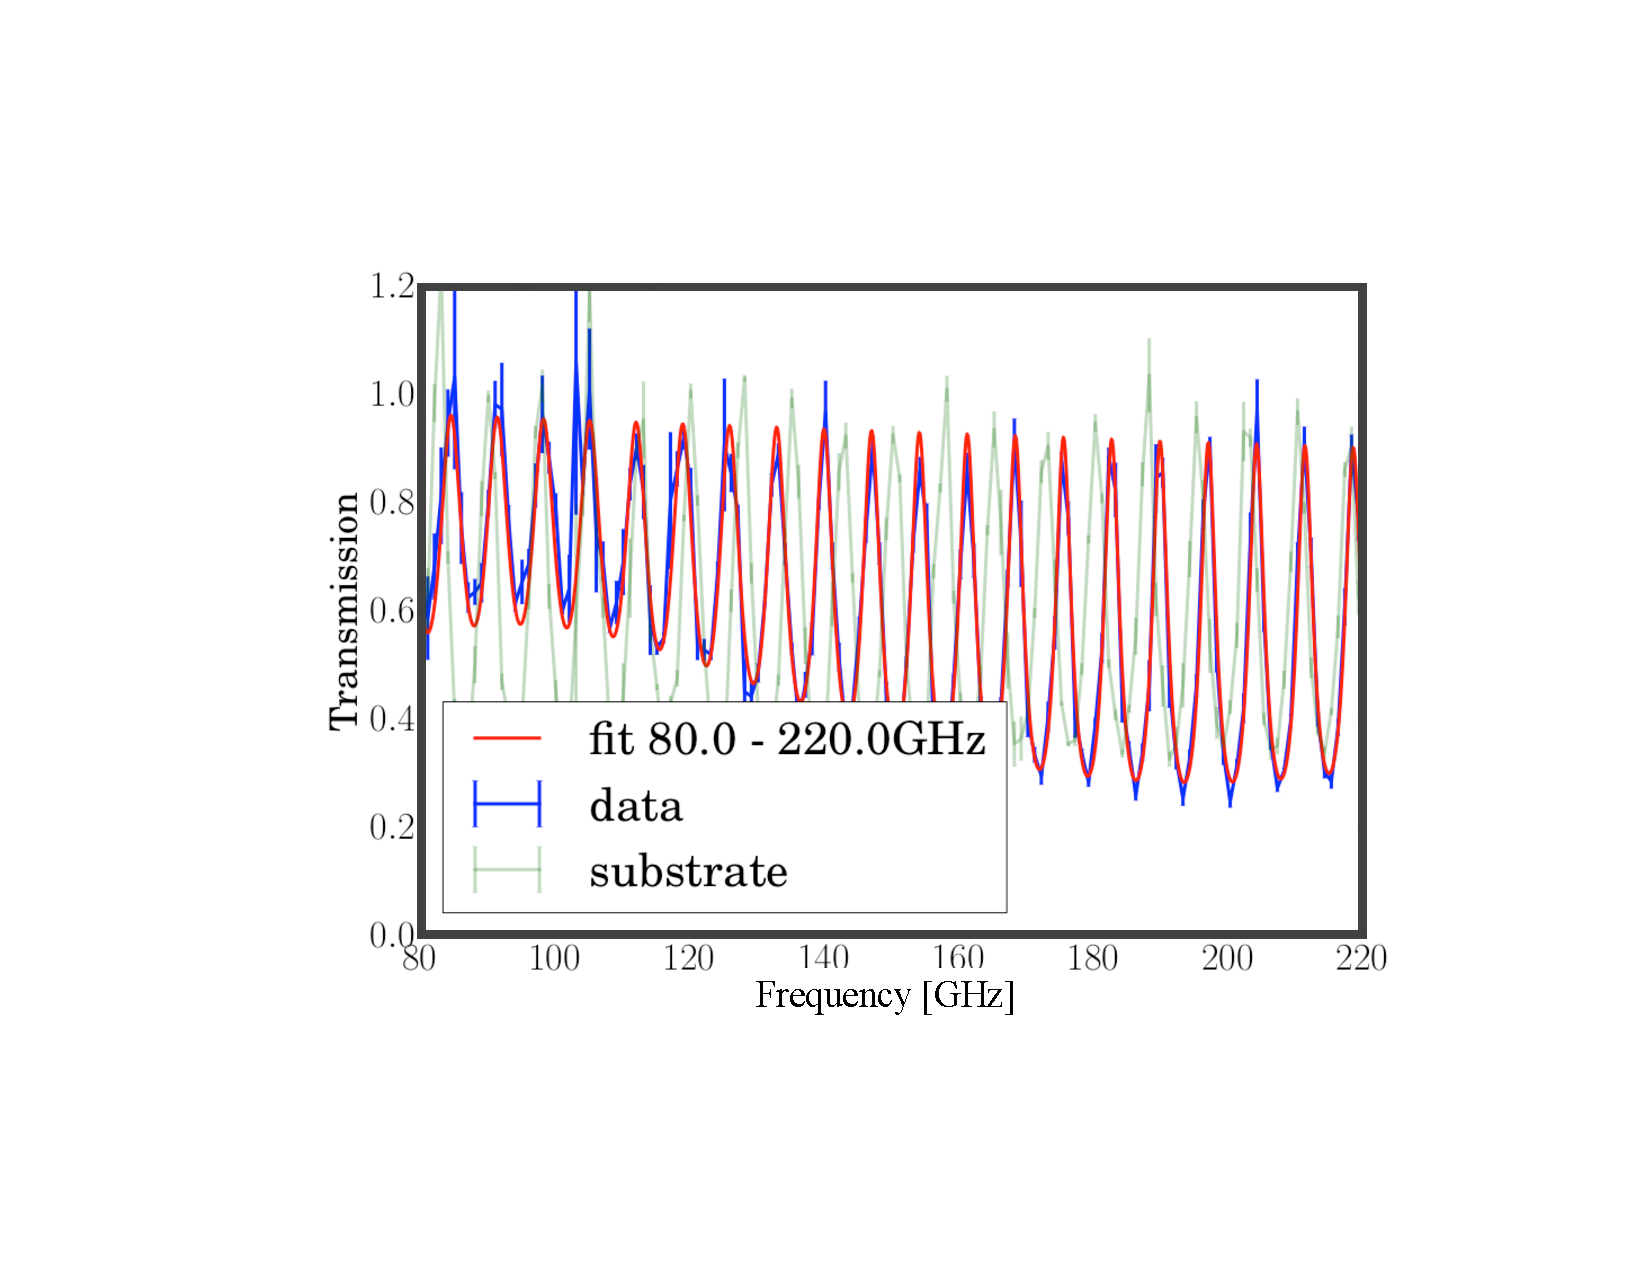
\includegraphics[width=0.48\linewidth, trim=5cm 4cm 4cm 3cm, clip]{PB2aWHWP/Figures/whwp_ar_ro3006.pdf}}
    \subfloat[\label{fig:pb2a_whwp_ar_layers:b}]{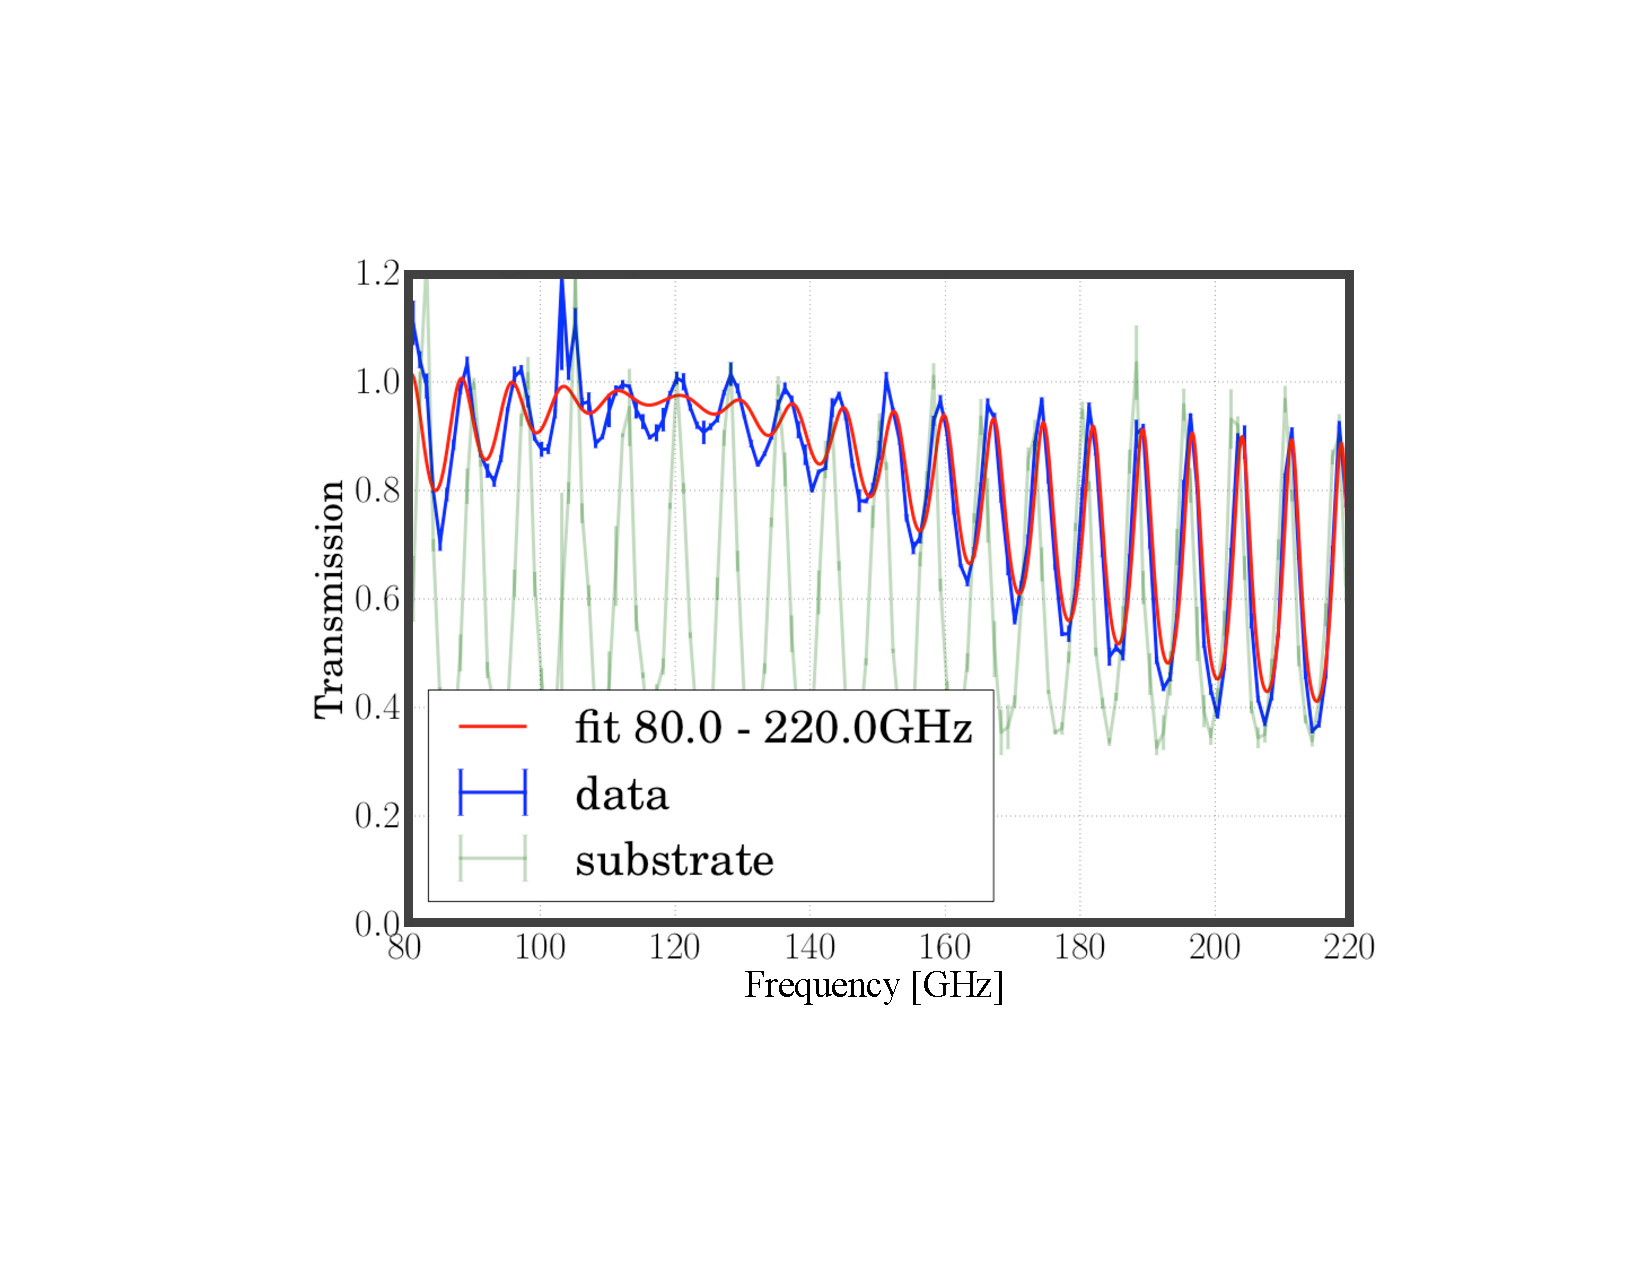
\includegraphics[width=0.48\linewidth, trim=5cm 4.2cm 4cm 2.8cm, clip]{PB2aWHWP/Figures/whwp_ar_hdpe.pdf}}
    \caption[AR coating candidates for the PB-2a WHWP and their measured indexes and loss tangents, as well as the measured spectra of selected materials.]{The table presents measured indexes and loss tangents for candidate AR materials using UC Berkeley FTS data. Because the films are thin, they were pressed onto an alumina substrate, and the spectra were compared to that without the AR film. The selected materials are bolded: HDPE for the top layer, RO3006 for the bottom layer. Figures~\ref{fig:pb2a_whwp_ar_layers:a} and~\ref{fig:pb2a_whwp_ar_layers:b} show the measured FTS spectra between 80 and 220~GHz for the RO3006 (left panel) and HDPE (right panel). Blue lines show the alumina$+$film fringe, the green line shows the alumina-alone fringe, and the red line shows the fit. The ``fast'' fringe pattern is due to the $\sim$1/4" alumina substrate, and the ``slow'' modulation of the fast fringe is used to extract the AR layer's refractive index.}
    \label{fig:pb2a_whwp_ar_layers}
\end{figure}

As shown in Figure~\ref{fig:ar_layers}, HDPE has an index of $n_{\mathrm{HDPE}} = 1.55$ while the Duroid has an index of $n_{\mathrm{3006}} = 2.52$. Both of these indexes are substantially larger than the targets of $(n_{\mathrm{top}}, n_{\mathrm{bot}}) = (1.40, 2.31)$, which in turn increases its reflectivity compared to the idealized case. In addition, such thin plastics are difficult to machine\footnote{The difficulty of machining the AR coatings is in part because we do not glue them down, as discussed later in this section. If we had instead glued the coatings to the flat, rigid sapphire windows, they would have been more easily tuned using a CNC. See Section~blah for more details about plastic AR machining.} due to their being flimsy and therefore difficult to fixture, an for this reason, PB-2a uses both the HDPE and RO3006 at stock thickness, which are $\approx$~25~$\mathrm{\mu m}$ thicker than optimal. This choice programmatically motivated design feature facilitated the on-time arrival of the WHWP to meet the PB-2a receiver in Chile.

\begin{figure}[!t]
    \centering
    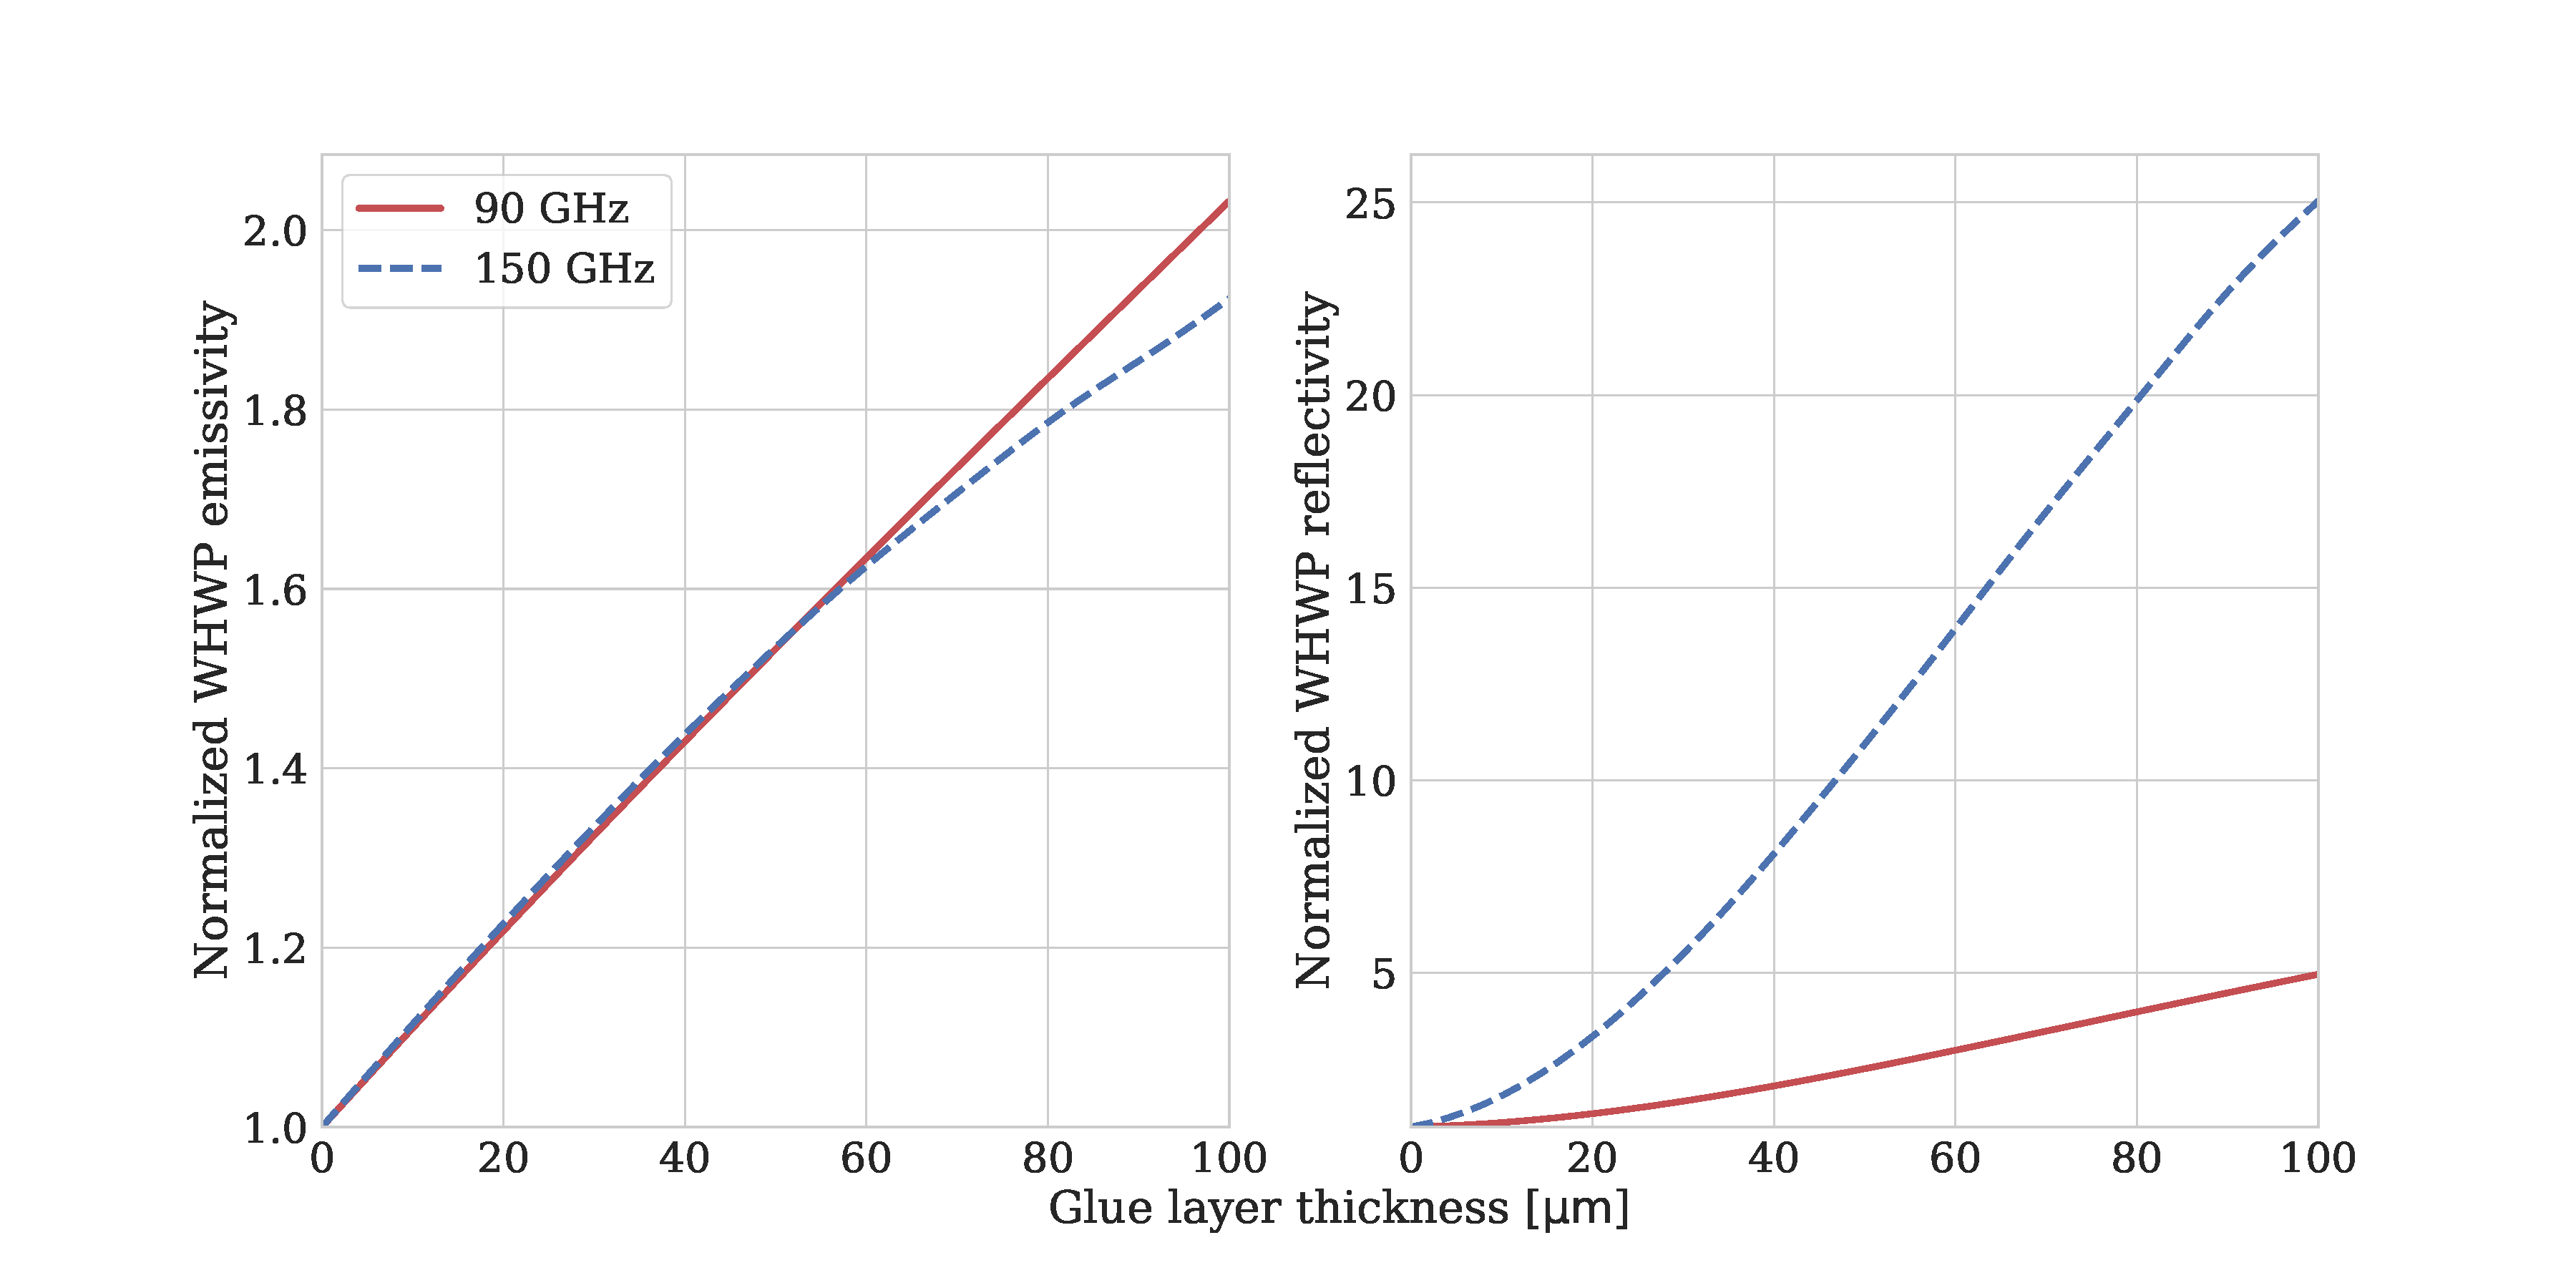
\includegraphics[width=\linewidth, trim=3cm 1cm 3cm 3cm, clip]{PB2aWHWP/Figures/pb2a_whwp_glue_layer_impact.pdf}
    \caption[Impact of a potential glue layer on PB-2a WHWP emissivity and reflectivity.]{The impact of a potential epoxy glue layer, assumed to have an index of $n_{\mathrm{glue}} = 1.7$ and an ambient-temperature loss tangent of $\tan \delta = 0.01$, on the emissivity and reflectivity of the WHWP. Because the glue layers create index mismatches, reflectivity increases sharply with glue thickness, especially at 150~GHz.}
    \label{fig:pb2a_whwp_glue_layer_impact}
\end{figure}

Because minimizing emissivity and reflectivity is central to the AR coating design, the impact of adhesive layers is a major concern for the WHWP's construction. A typical practice throughout the CMB field is to affix plastic AR layers using an adhesive such as epoxy or rubber cement.\footnote{Low-density polyethylene (LDPE) is also often used as a uniform, low-loss adhesive by heat pressing the AR coating onto the optic above the LDPE's melting temperature. This technique for 500~mm-diameter optics is difficult and requires substantial, dedicated infrastructure and therefore was not considered deeply for PB-2a.} While adhesives are relatively straightforward to implement during fabrication, they introduce several complications to the optical assembly. First, the glue adds additional dielectric layers between the AR layers and the sapphire windows. In order for these layers to impact WHWP's reflectivity negligibly, they must be much thinner than the wavelength of interest. As an example, generic epoxy\footnote{``Generic'' describes epoxies without any fillers, such as Stycast 1266.} typically has a refractive index of $n = 1.7$, which causes index mismatches throughout the stack that are especially large between the sapphire windows.\footnote{Because sapphire is not infinitely rigid, clamping an unadhered sapphire stack at its edge causes the first and third pieces to bow away form the second, which in turn creates $\sim 100$~$\mathrm{\mu m}$ gaps between the sapphire windows.} In addition, adhesives are quite lossy at room temperature ($\tan \delta \sim 10^{-2}$), which also necessitates a very thin layer to avoid degrading instrument performance. Figure~\ref{fig:pb2a_whwp_glue_layer_impact} shows WHWP emissivity and reflectivity as function of glue layer thickness, and even a 20~$\mathrm{\mu m}$ substantially increases both WHWP reflection and absorption.

Second, adhesive layers are difficult to make uniform. This is in contrast to other layers in the WHWP's optical stack, which are specifically fabricated for uniformity (extrusion for the plastic AR layer, and HEM growth for the sapphire). Therefore, the adhesive layer is the most likely optical-stack element to create position-dependent emissivity which in turn generates HWPSSs. Third, ambient temperature typically fluctuates between $-20^{\circ}$ to $20^{\circ}$ at the Chile site, and every time the sun rises and sets, the WHWP expands and contracts, stressing the bond between the AR layers and sapphire windows, which have different coefficients of thermal expansion (CTEs). This repeated stress can lead to progressive AR delamination during the course of PB-2a's lifetime that can be difficult to detect during in-situ data quality assessment.

\begin{figure}[!t]
    \centering
    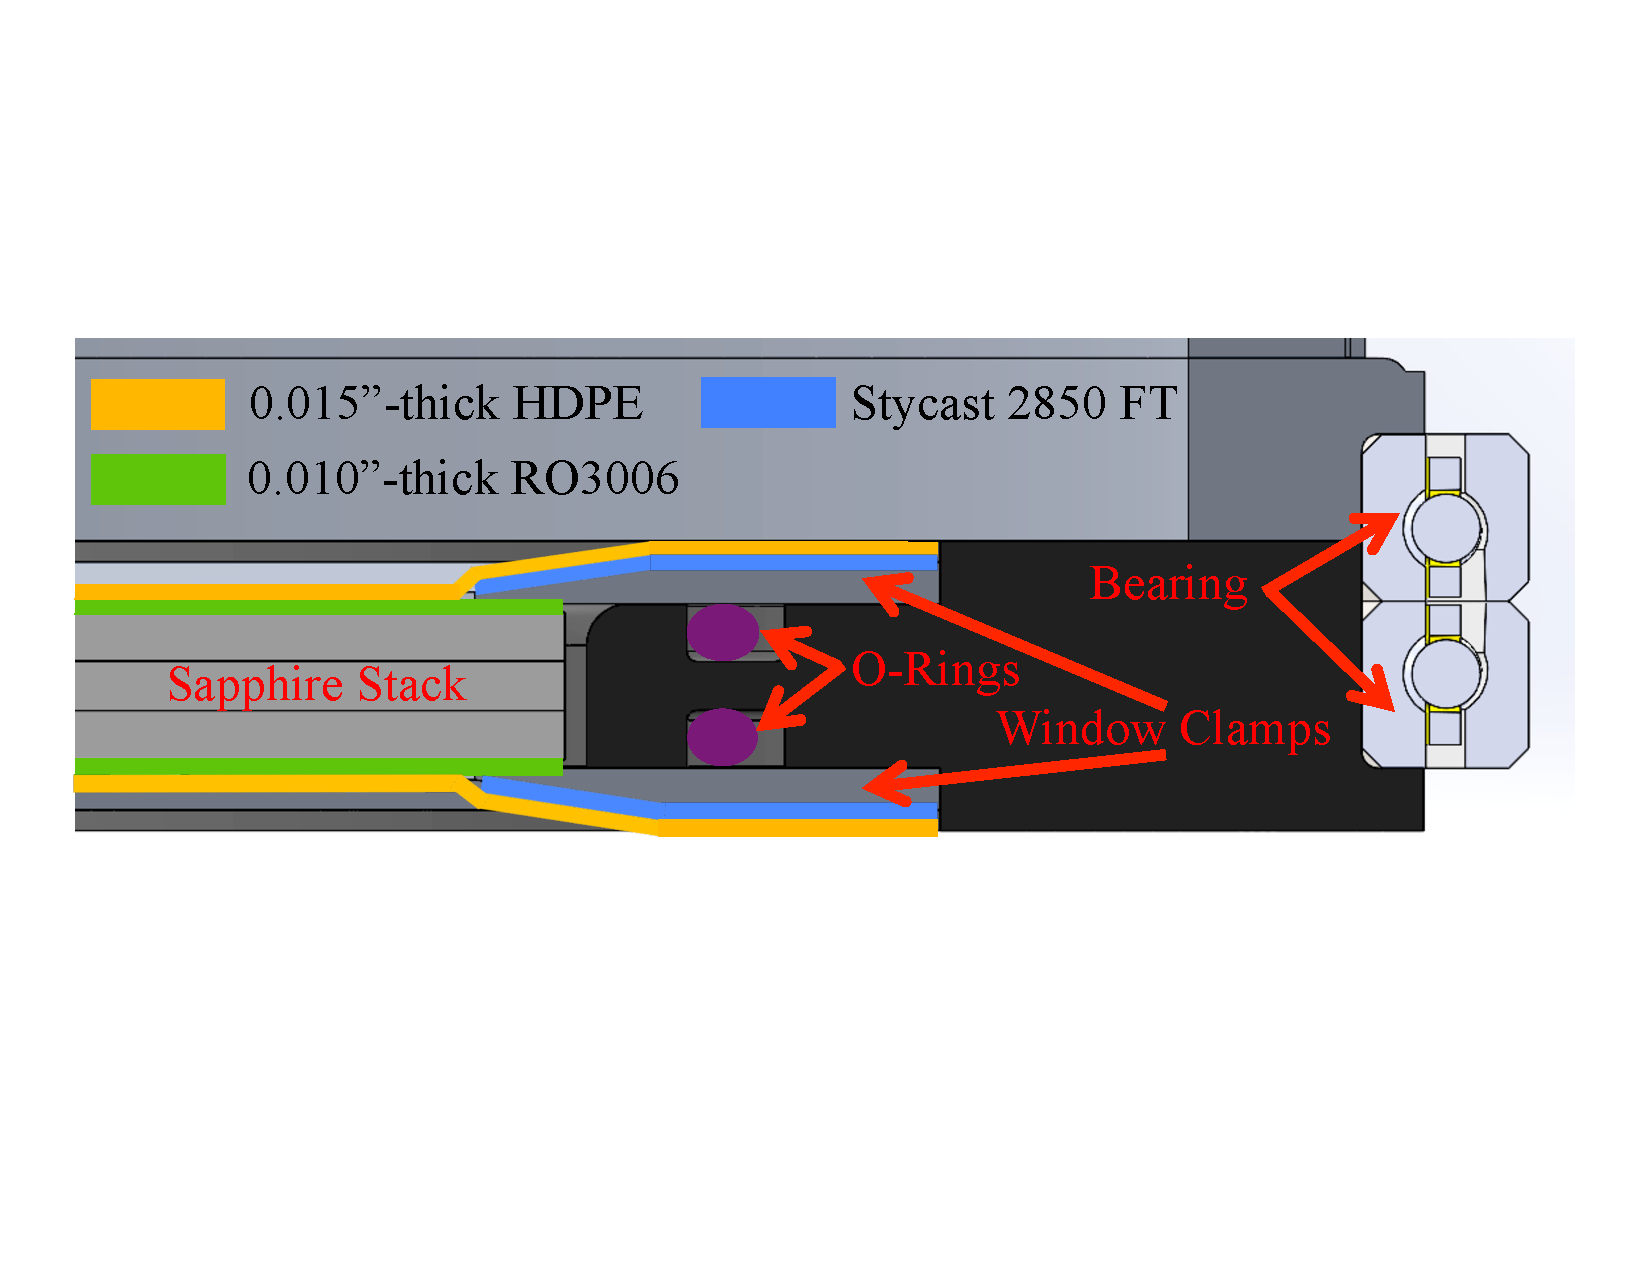
\includegraphics[width=0.8\linewidth, trim=1cm 7cm 2cm 6cm, clip]{PB2aWHWP/Figures/pb2a_whwp_ar_coating_vacuum_bag.pdf}
    \caption{A cross-sectional view of the vacuum module. The HDPE AR layers are glued to aluminum annuli which mate to o-ring seals on the rotor. When the module is evacuated, atmospheric pressure presses the AR layers onto the sapphire, eliminating the need for glue layers.}
    \label{fig:pb2a_whwp_vacuum_bagging}
\end{figure}

For the reasons laid out above, we press the AR coating and sapphire windows together using a vacuum bagging technique in order to avoid adhesives. A cross sectional CAD drawing of the AR coating assembly is shown in Figure~\ref{fig:pb2a_whwp_vacuum_bagging}, and a photo of the fully-assembled WHWP, including the AR coating, is shown in Figure~\ref{fig:whwp_assem}. The basic principle of the bagging method is to create a vacuum space using the outermost HDPE layers such that ambient pressure forces the sapphire stack and AR layers together. Each HDPE sheet is glued using Stycast 2850FT\footnote{Stycast 2850FT is often used to seal vacuum spaces, and because its CTE is matched to that of aluminum, the integrity of its seal is (empirically) robust to ambient temperature variations.} to an aluminum ``window clamp'' ring, which in turn interfaces to the rotor stage via o-rings to create a seal, and the bag is pumped out via a valved vacuum port. Maintaining sufficiently low pressure for $\sim$months of continuous operation is challenging due to the vacuum chamber's having a relatively small volume. Therefore, a tubular chamber was added to the rotor to increase the low-pressure volume and is shown in Figure~\ref{fig:whwp_assem:b}.

%%%%%%%%%%%%%%%%%%%%%%%%%%%%%%%%
%%%%%%%%%%%%%%%%%%%%%%%%%%%%%%%%
%%%%%%%%%%%%%%%%%%%%%%%%%%%%%%%%

\section{Mechanical assembly}
\label{sec:pb2a_whwp_mechanical_assembly}

The WHWP mount and rotation stage must spin the 500~mm-diameter optical stack at 2~Hz more than 100~million times throughout PB-2a's observational lifetime. Furthermore, the HWP assembly must minimize vibrational coupling to the telescope and receiver, maintain adequate rotational stability, accommodate in-field optical alignment, and be robust against mechanical failure. In this section, we describe several key features of the PB-2a HWP mechanical assembly shown in Figure~\ref{fig:whwp_assem}.

\begin{figure}[!t]
    \centering
    \subfloat[\label{fig:whwp_assem:a}]{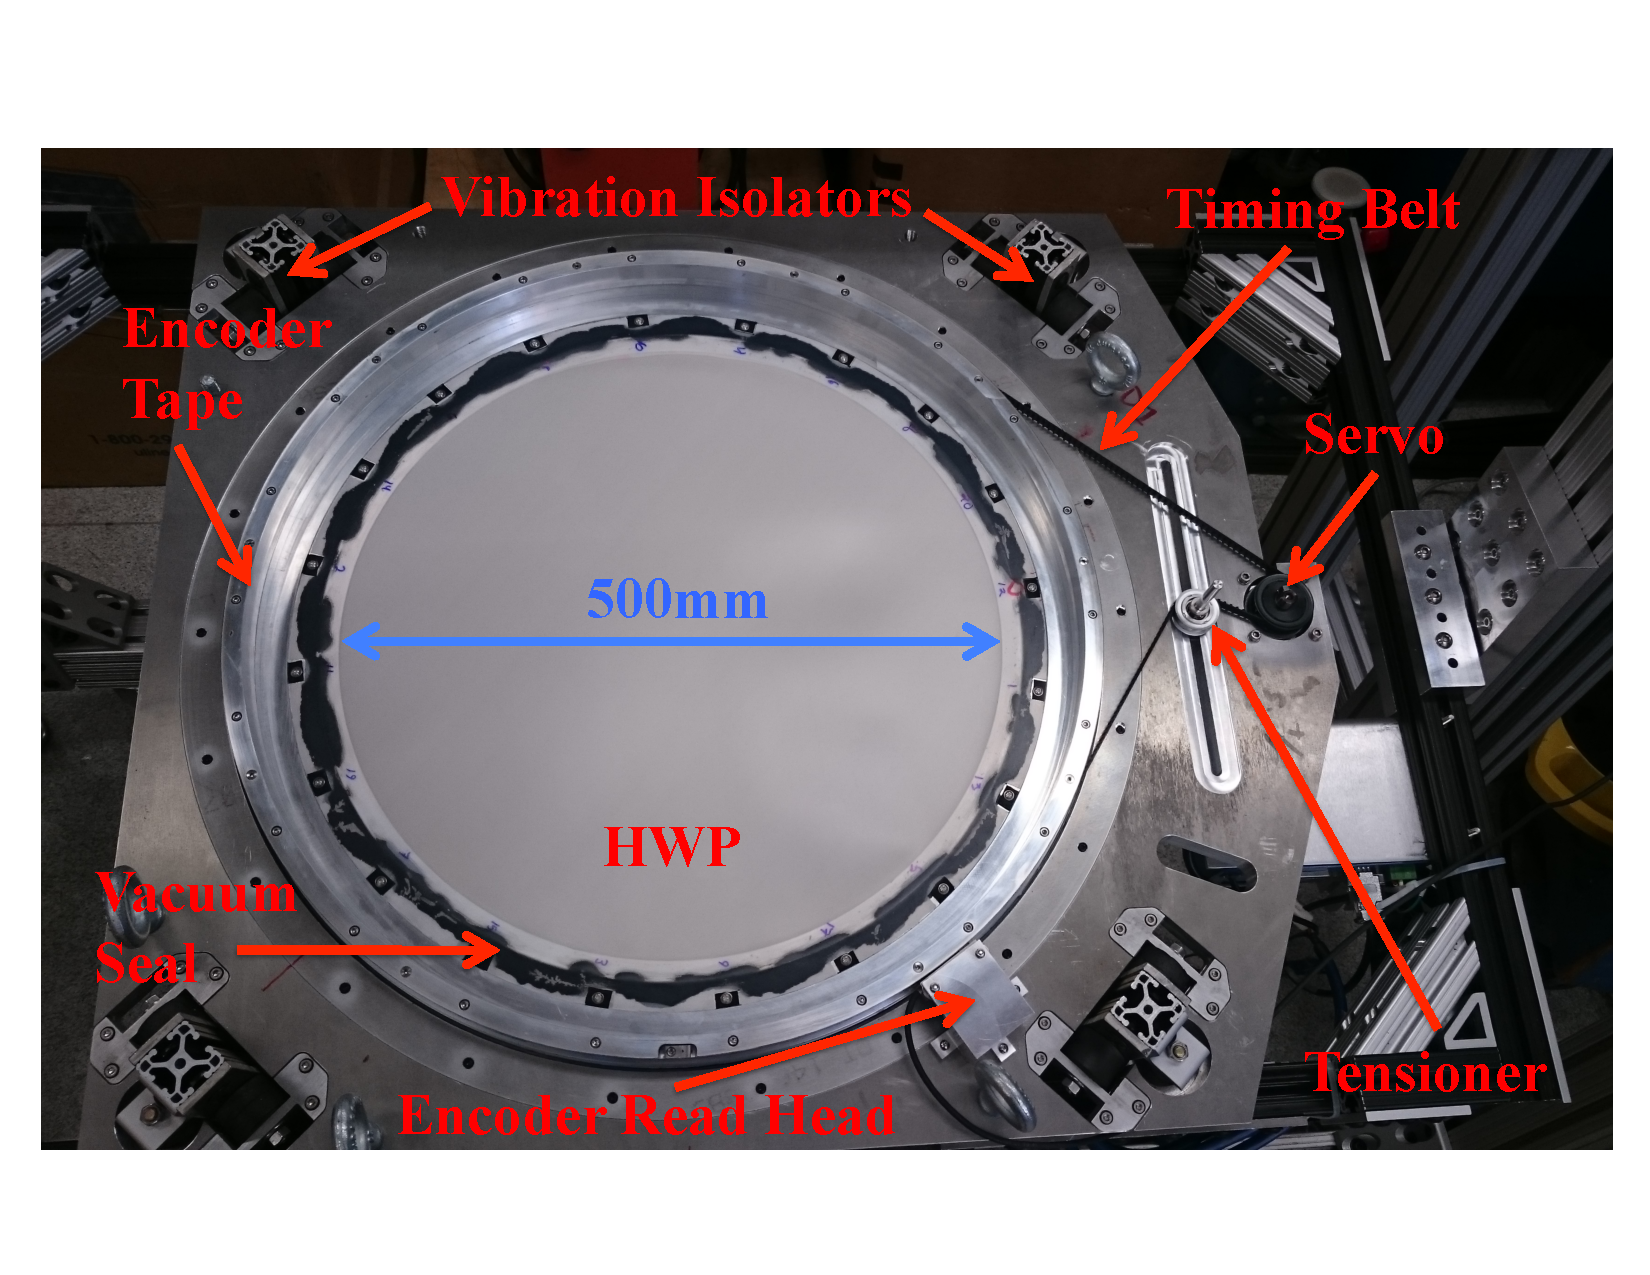
\includegraphics[width=0.48\linewidth, trim=1.5cm -1.5cm 1.5cm 2cm, clip]{PB2aWHWP/Figures/WHWP_photo.pdf}}
    \subfloat[\label{fig:whwp_assem:b}]{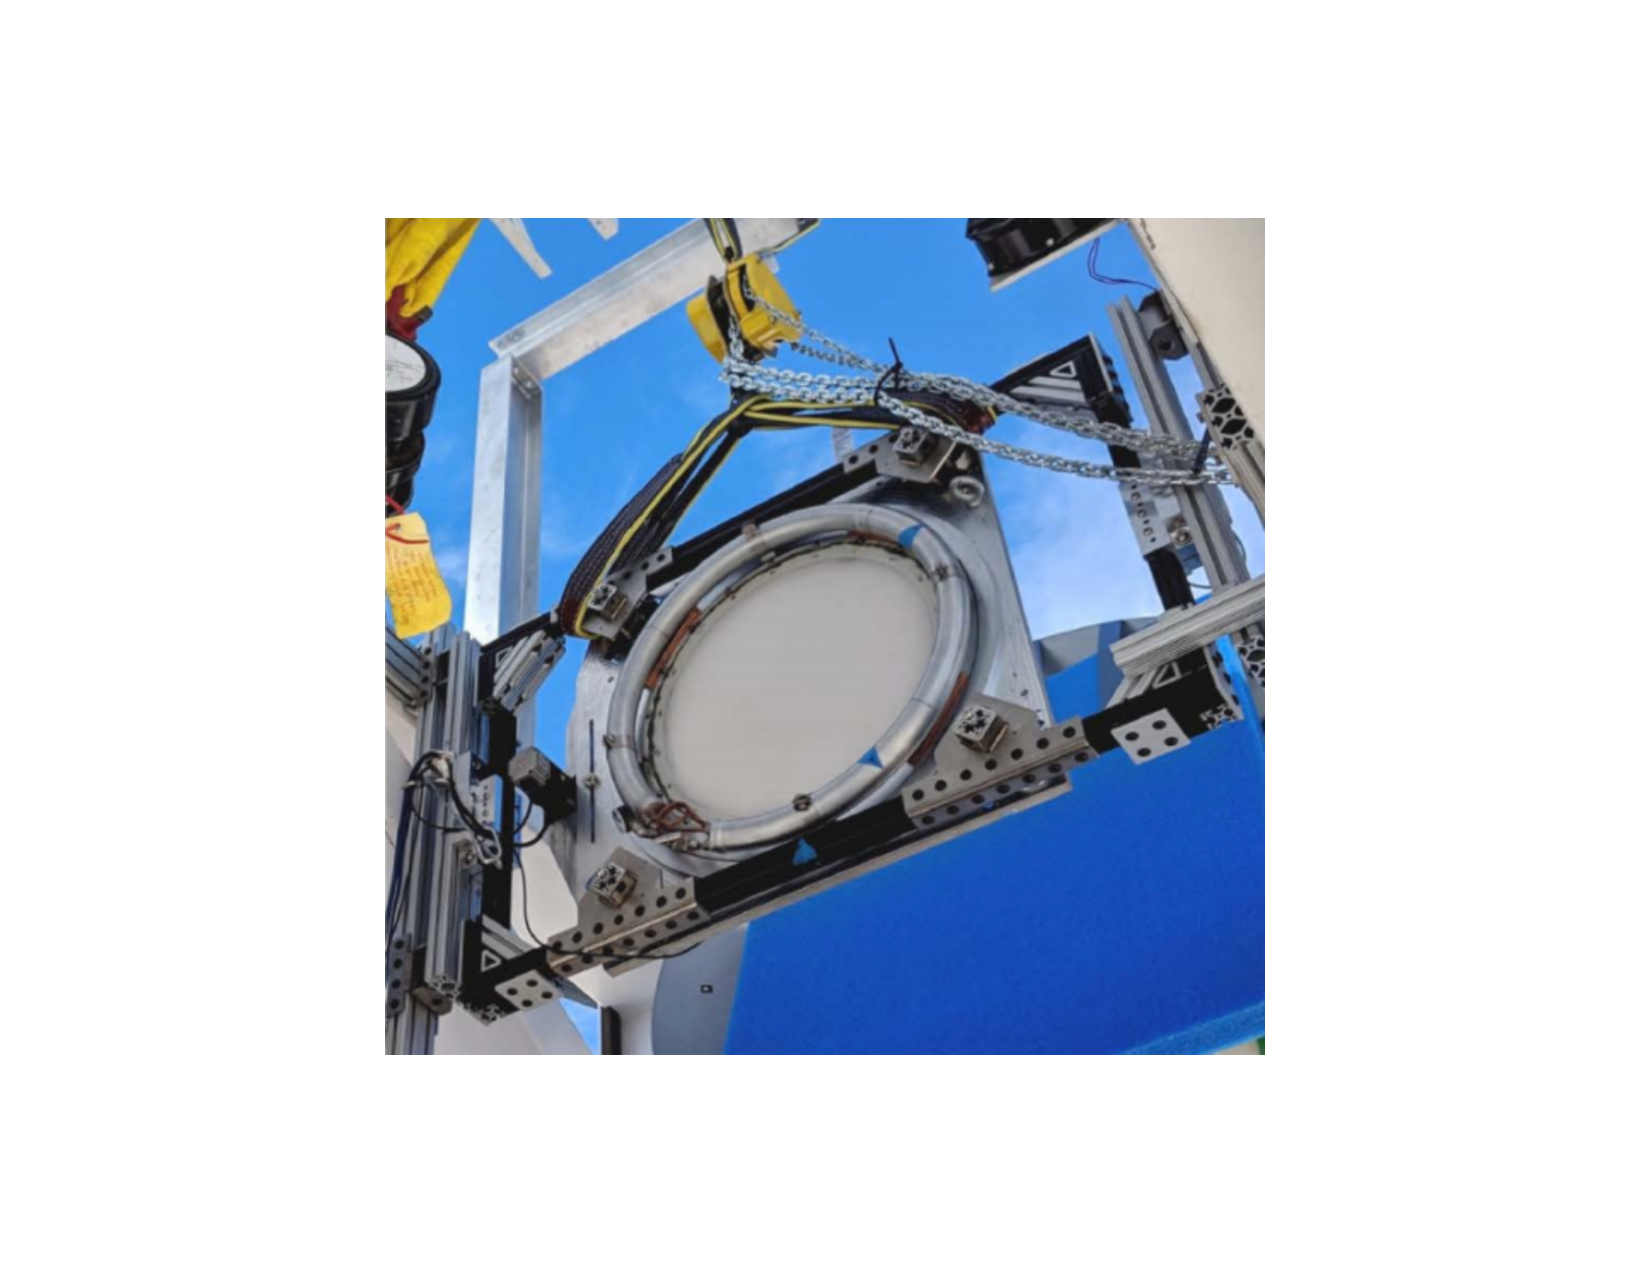
\includegraphics[width=0.48\linewidth,trim=6cm 4cm 8cm 4cm, clip]{PB2aWHWP/Figures/pb2a_whwp_hoisted.pdf}}
    \caption[Photos of the PB-2a WHWP mechanical assembly.]{Photos of the PB-2a WHWP mechanical assembly. \ref{fig:whwp_assem:a} a shows the fully-assembled HWP on its teststand at Berkeley. Important aspects of the design include a vacuum module to apply the AR coating, a servo motor coupled to a timing belt for modularity and rotational stability, and vibration damping mounts to mechanically isolate the HWP from the receiver cryostat. \ref{fig:whwp_assem:b} shows the WHWP mounted on the PB-2a telescope. The secondary mirror is covered with blue foam, and the receiver cryostat was not yet installed during this test fit. The tubular structure on the rotor adds volume to the AR vacuum bag.}
    \label{fig:whwp_assem}
\end{figure}

%%%%%%%%%%%%%%%%%%%%%%%%%%%%%%%%
%%%%%%%%%%%%%%%%%%%%%%%%%%%%%%%%

\subsection{Mount}
\label{sec:pb2a_whwp_mount}

The WHWP mount is designed to maximize configurational flexibility and minimize rotation-induced vibrations coupled to the telescope. The mount attaches to the telescope's boom via a series of 80/20 rails and rotational stages, allowing for fine control along three translational and two rotational axes. Additionally, the mount is capable of positioning the HWP either in front of the cryostat window or between the primary and secondary mirrors, as in PB-1. This locational flexibility allows for in situ evaluation of HWP-related aberrations, instrumental polarization, and beam coverage. In order to ensure that WHWP vibrations are isolated from the telescope and vice versa, the assembly is coupled to the telescope using a series of independent rubber sandwich mounts oriented both tangentially and axially to the HWP rotation axis. To isolate the sapphire from vibrations in the bearing, the optical stack is clamped by a thin rubber gasket.

%%%%%%%%%%%%%%%%%%%%%%%%%%%%%%%%
%%%%%%%%%%%%%%%%%%%%%%%%%%%%%%%%

\subsection{Rotation stage}
\label{sec:pb2a_whwp_rotation_stage}

The WHWP rotation stage comprises a large-bore bearing, a timing-belt-coupled gear system, and a servo motor. For rotor-stator coupling, we employ a 635~mm-diameter matched-pair thin-section ball bearing from SilverThin
Bearings\footnote{SilverThin Bearings: http://www.silverthin.com/}. This bearing is a scaled-up version of that used on PB-1 and is chosen for its demonstrated success at the observation site. The bearing is preloaded to meet product specifications and is lubricated with a low-temperature-compatible grease to accommodate on-site weather conditions. The bearing's races are stainless steel, and the bearing clamps are 7075 aluminum to minimize weight. To validate mechanical compatibility with Chilean conditions, we perform bearing stress and thermal tests to ensure robustness against premature wear and seizing. 

The drivetrain is a 400~W, 60~mm AC servo from Applied Motion Products\footnote{Applied Motion: http://www.applied-motion.com/}. This motor accommodates our estimated peak and continuous torque requirements with a safety factor of $\approx$~3 and avoids electrical switching noise present in comparable stepper motors. The servo is tuned to provide loose feedback, keeping the motor from overheating and utilizing the rotor’s large moment of inertia to maintain stable rotation. The drivetrain is connected to the rotor via a Kevlar-reinforced timing belt and a commercial tensioner pulley, a system that allows for easy installation of replacement parts at the observation site. When on the telescope, the WHWP operates in the weatherproofed receiver enclosure, making it safe from winds and snow but not from fluctuations in ambient temperature. Therefore, all WHWP components are rated to $-20^{\circ}$~C.

%%%%%%%%%%%%%%%%%%%%%%%%%%%%%%%%
%%%%%%%%%%%%%%%%%%%%%%%%%%%%%%%%

\subsection{Angle encoder}
\label{sec:pb2a_whwp_angle_encoder}

In order to suppress jitter in the WHWP angle reconstruction that can add noise during the analysis process, we must achieve a timing resolution much finer than 10~ms, which would be the digitization noise level if we naively read out the encoder at the 100~Hz detector sampling rate. We utilize a commercial optical encoder from RSF Elektronik\footnote{RSF: http://www.rsf.at/en/} that consists of a steel tape with 10,000 reflective lines and an infrared read head, as shown in Figure~\ref{fig:pb2a_whwp_encoder:a}. The encoder tape is mounted on a 636~mm-diameter aluminum ring such that its surface maintains a radial distance of 0.75~$\pm$~(0.4, 0.2)~mm from the read head during WHWP rotation. This system provides 6.5~arcsec resolution via 4-times interpolation.

\begin{figure}[!t]
    \centering
    \subfloat[\label{fig:pb2a_whwp_encoder:a}]{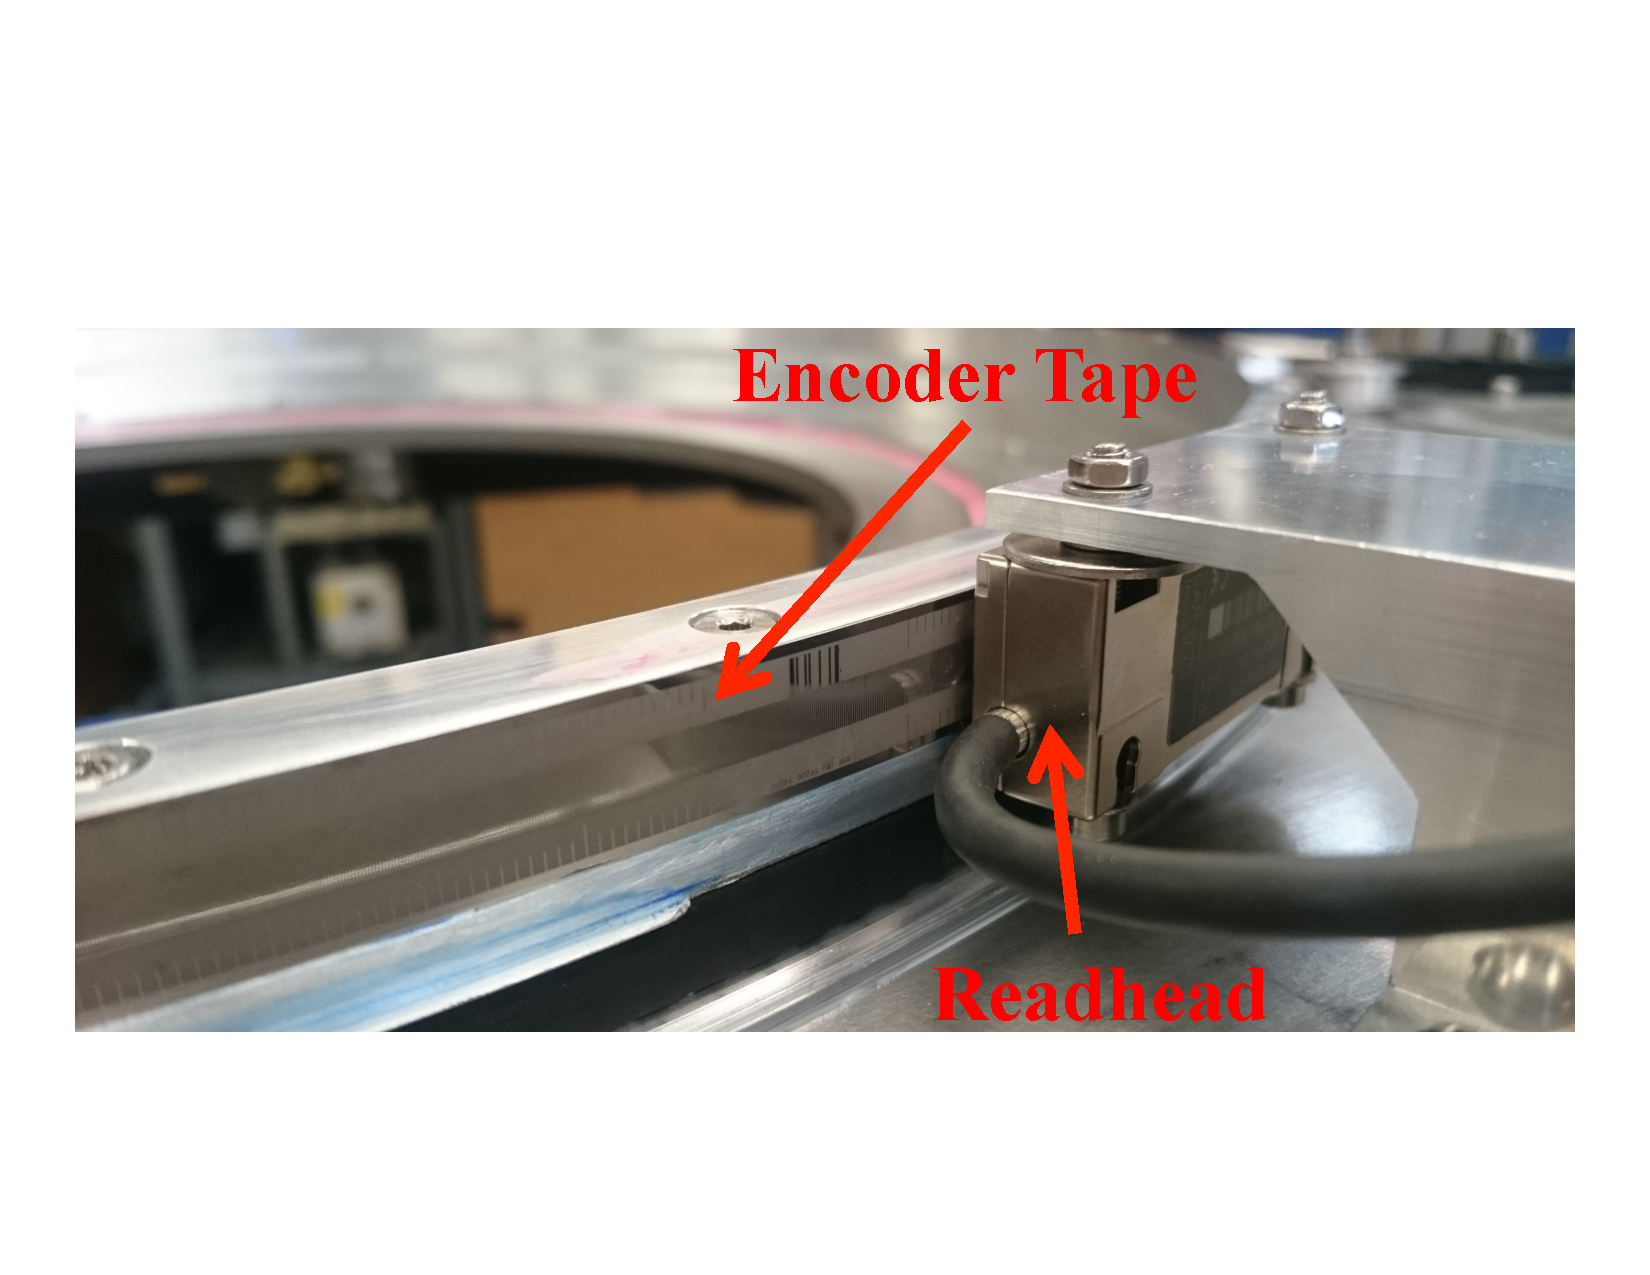
\includegraphics[width=0.48\linewidth, trim=5cm 0.5cm 3cm 5cm, clip]{PB2aWHWP/Figures/pb2a_whwp_encoder.pdf}}
    \subfloat[\label{fig:pb2a_whwp_encoder:b}]{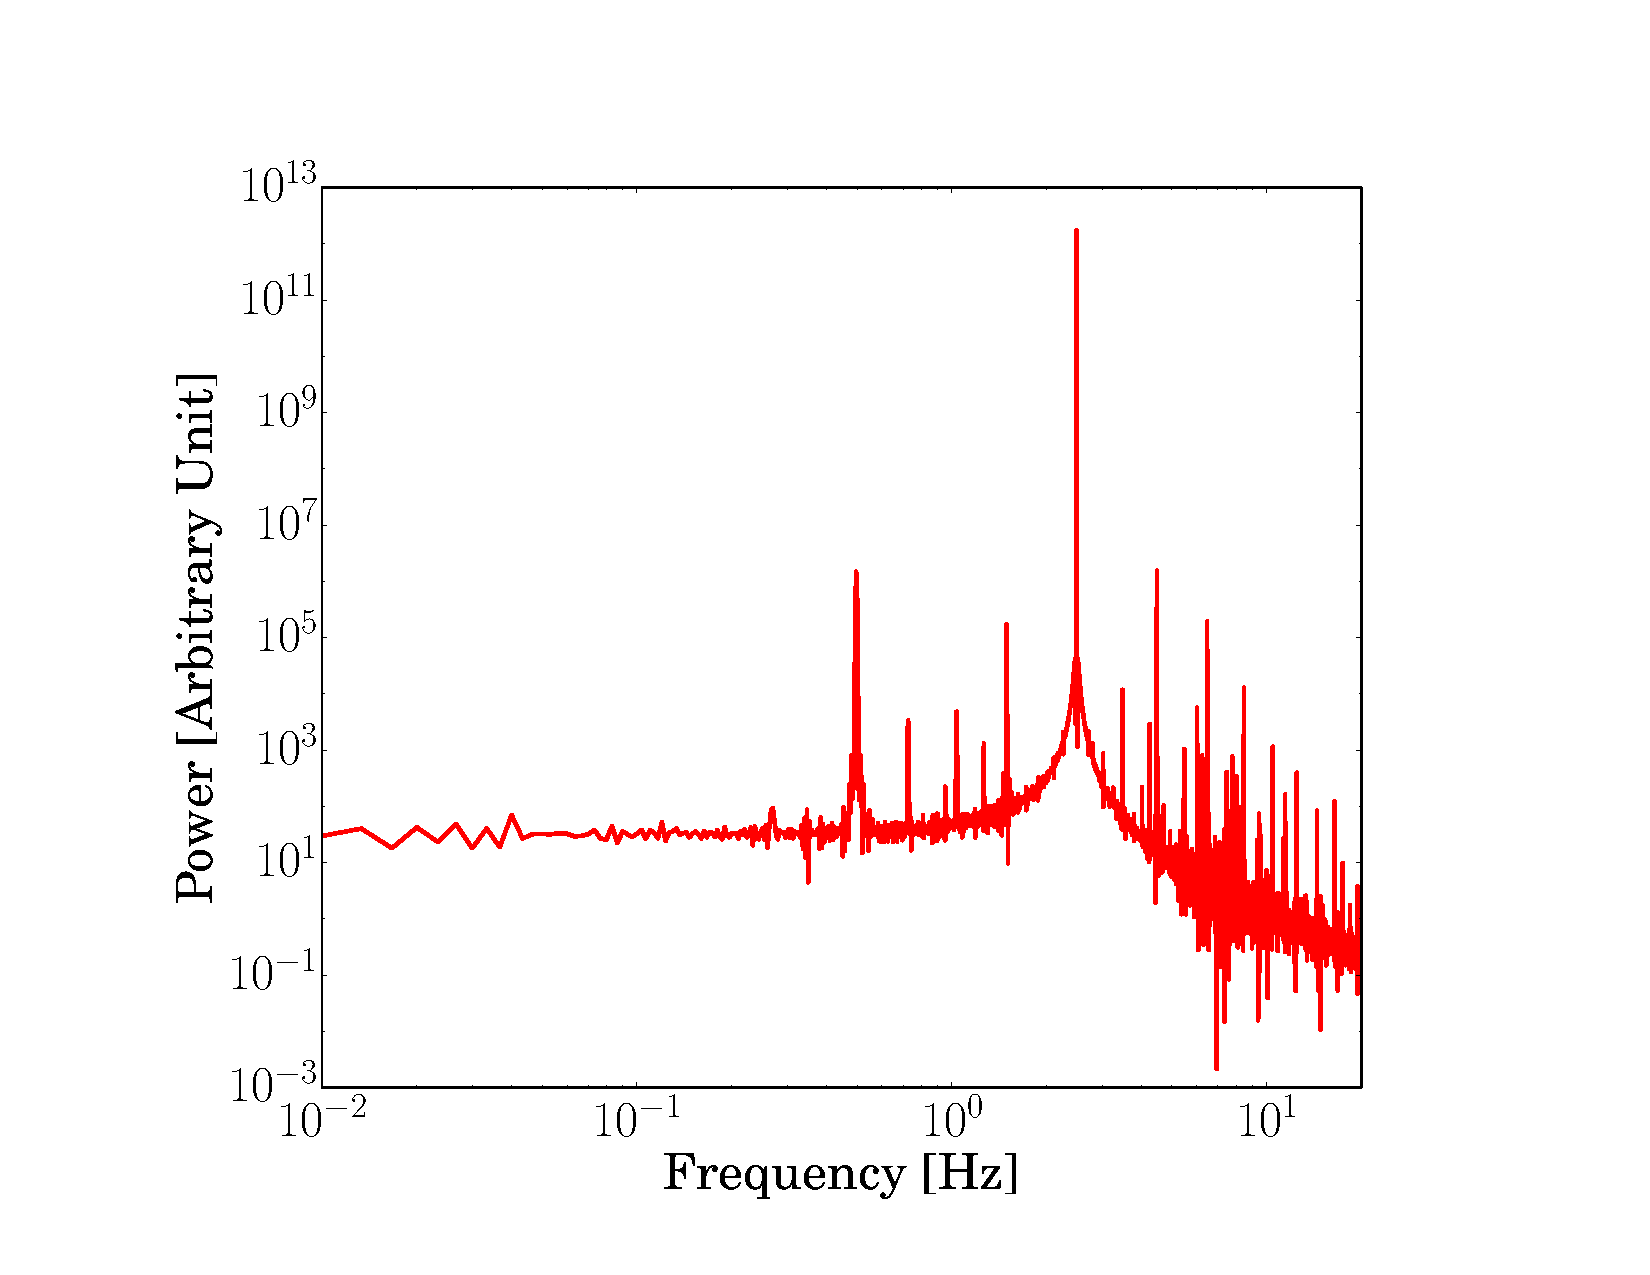
\includegraphics[width=0.48\linewidth, trim=2.5cm 1cm 4.5cm 2.5cm, clip]{PB2aWHWP/Figures/DrivePSD.pdf}}
    \caption[The PB-2a WHWP encoder mechanism and performance.]{Figure~\ref{fig:pb2a_whwp_encoder:a} shows a photograph of the encoder tape and read head. Read head gap tolerance is $+$~0.4~mm / $−$~0.2~mm, necessitating $<$~0.03 ellipticity for the 635~mm-diameter encoder tape mounting ring. Figure~\ref{fig:pb2a_whwp_encoder:b} shows a power spectral density of the HWP rotation at $\approx$~2.2~Hz over a five-minute period. The excellent rotational stability of the drive train demonstrates the effectiveness of the servo/timing belt system.}
    \label{fig:pb2a_whwp_encoder}
\end{figure}

To read out the encoder, we use an Arduino Leonardo ETH microcontroller. The Arduino samples the encoder signal at 40 kHz and averages the data down at the 100 Hz detector sampling to achieve WHWP angle resolution of
\begin{equation}
    \sigma_{\chi} = \frac{30 \, \mathrm{\mu rad}}{\sqrt{12}} \sqrt{\frac{1}{16 \times 10^{3} \, \mathrm{Hz}}} = 0.7 \, \frac{\mathrm{\mu rad}}{\sqrt{\mathrm{Hz}}} \, , 
\end{equation}
where $30 \, \mathrm{\mu rad} = 6.5$~arcsec is the encoder resolution, $1 / \sqrt{12}$ is the standard deviation of a uniform distribution for the Arduino's sampling randomly between encoder ticks, and 16~kHz is the Arduino sampling rate. This noise level meets the $\ll$~3~$\mathrm{\mu rad}$ requirement presented in Section~\ref{sec:angle_encoding_noise_requirement}. After collecting a set number of encoder ticks, the Arduino then compiles a UDP packet containing the HWP angle and a universal timestamp (IRIG) and sends it to a central computer where it is verified and paired with a matching data packet. Using a microcontroller eliminates the need for a WHWP-dedicated computer and allows for cheap, quick replacement in the case of failure at the site.

%%%%%%%%%%%%%%%%%%%%%%%%%%%%%%%%
%%%%%%%%%%%%%%%%%%%%%%%%%%%%%%%%

\subsection{Mechanical validation}
\label{sec:pb2a_whwp_mechanical_validation}

To validate the WHWP rotation mechanism, we evaluate vibration damping, bearing robustness, rotational stability, and the lifetime of the vacuum module. Figure~\ref{fig:pb2a_whwp_encoder:b} shows the power spectral density of $\approx$~2.2~Hz WHWP rotation read out at 16~kHz for five minutes. The sharpness of the central peak demonstrates outstanding rotational stability and therefore validates the effectiveness of the servo/timing belt system. We run the WHWP continuously in the lab for $\sim$~1~week, checking the pressure in the AR vacuum assembly before and after the test to ensure that the act of rotation does not affect the rate of pressure change. In addition, after the WHWP moved to the Chile site, we tested it outdoors to ensure that it is indeed robust to ambient conditions and fitted it to the telescope before the receiver was installed, as shown in Figure~\ref{fig:whwp_assem:b}. WHWP vibration of the telescope structure was found to be negligible.

%%%%%%%%%%%%%%%%%%%%%%%%%%%%%%%%
%%%%%%%%%%%%%%%%%%%%%%%%%%%%%%%%
%%%%%%%%%%%%%%%%%%%%%%%%%%%%%%%%

\section{Optical evaluation}
\label{sec:pb2a_whwp_optical_evaluation}

As described in Section~\ref{sec:pb2a_whwp_emissivity_relfectivity_requirements}, the primary merit figures for the PB-2a WHWP performance are transmissivity, emissivity, and linear polarization modulation efficiency. There are two different modes we use to evaluate optical performance, which are cross-checked for consistency. In the first mode, we evaluate the optical properties of each optical-stack component. The AR evaluation is presented in Section~\ref{sec:pb2a_whwp_ar_coating}, so in this section we focus on the evaluation of the sapphire loss tangent, index, and crystal axis orientation. Measured sapphire and AR optical constants are in the table in Figure~\ref{fig:pb2a_whwp_mod_eff_spectrum}, and these individual-layer index and loss values can be used to simulate the performance of the assembled WHWP. In the second mode, we measure both transmissivity and band-averaged modulation efficiency of the assembled optical stack directly. In this section, we present the details of these measurements as well as their implications for the WHWP's performance in the field.

\begin{figure}[!t]
    \centering
    \subfloat[\label{fig:pb2a_whwp_mod_eff_spectrum:a}]{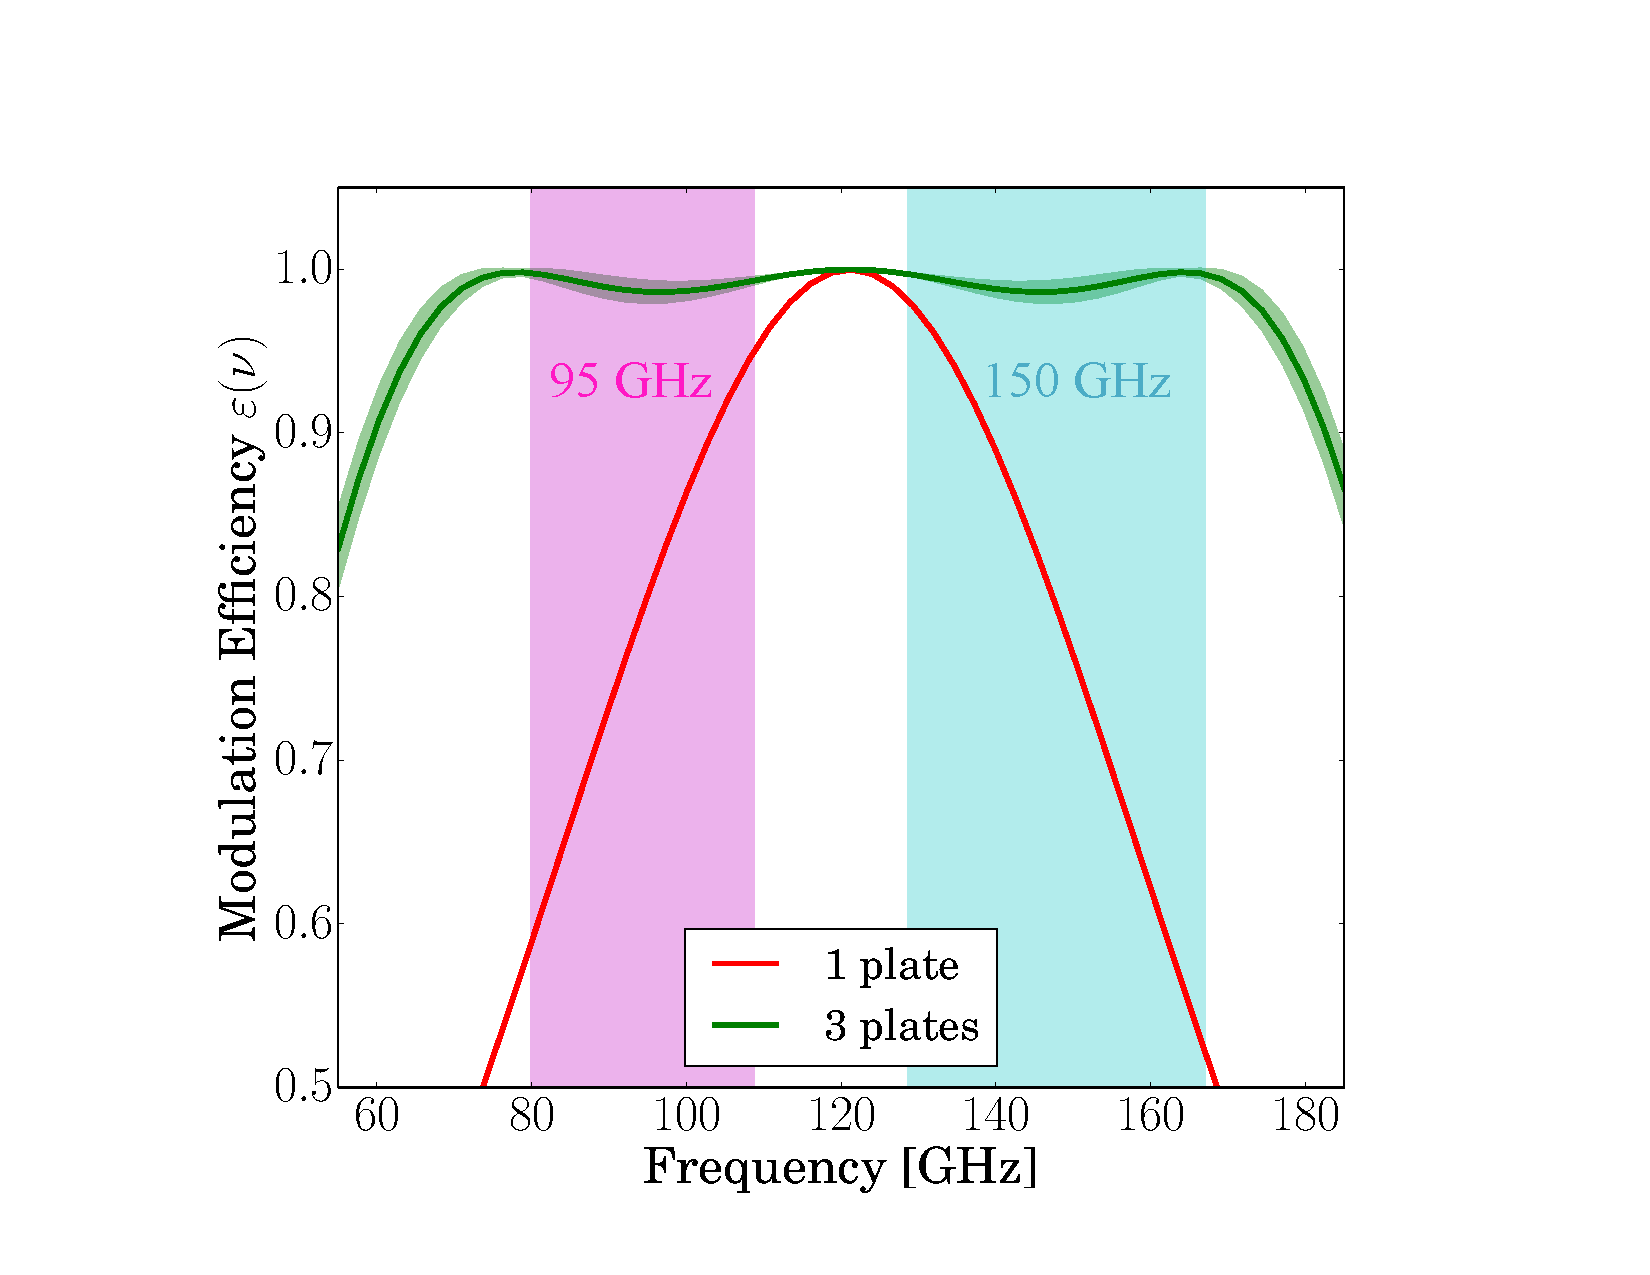
\includegraphics[width=0.48\linewidth, trim=3.5cm 1cm 5cm 2.8cm, clip]{PB2aWHWP/Figures/HWP_ModEff.pdf}}
    \subfloat[\label{fig:pb2a_whwp_mod_eff_spectrum:b}]{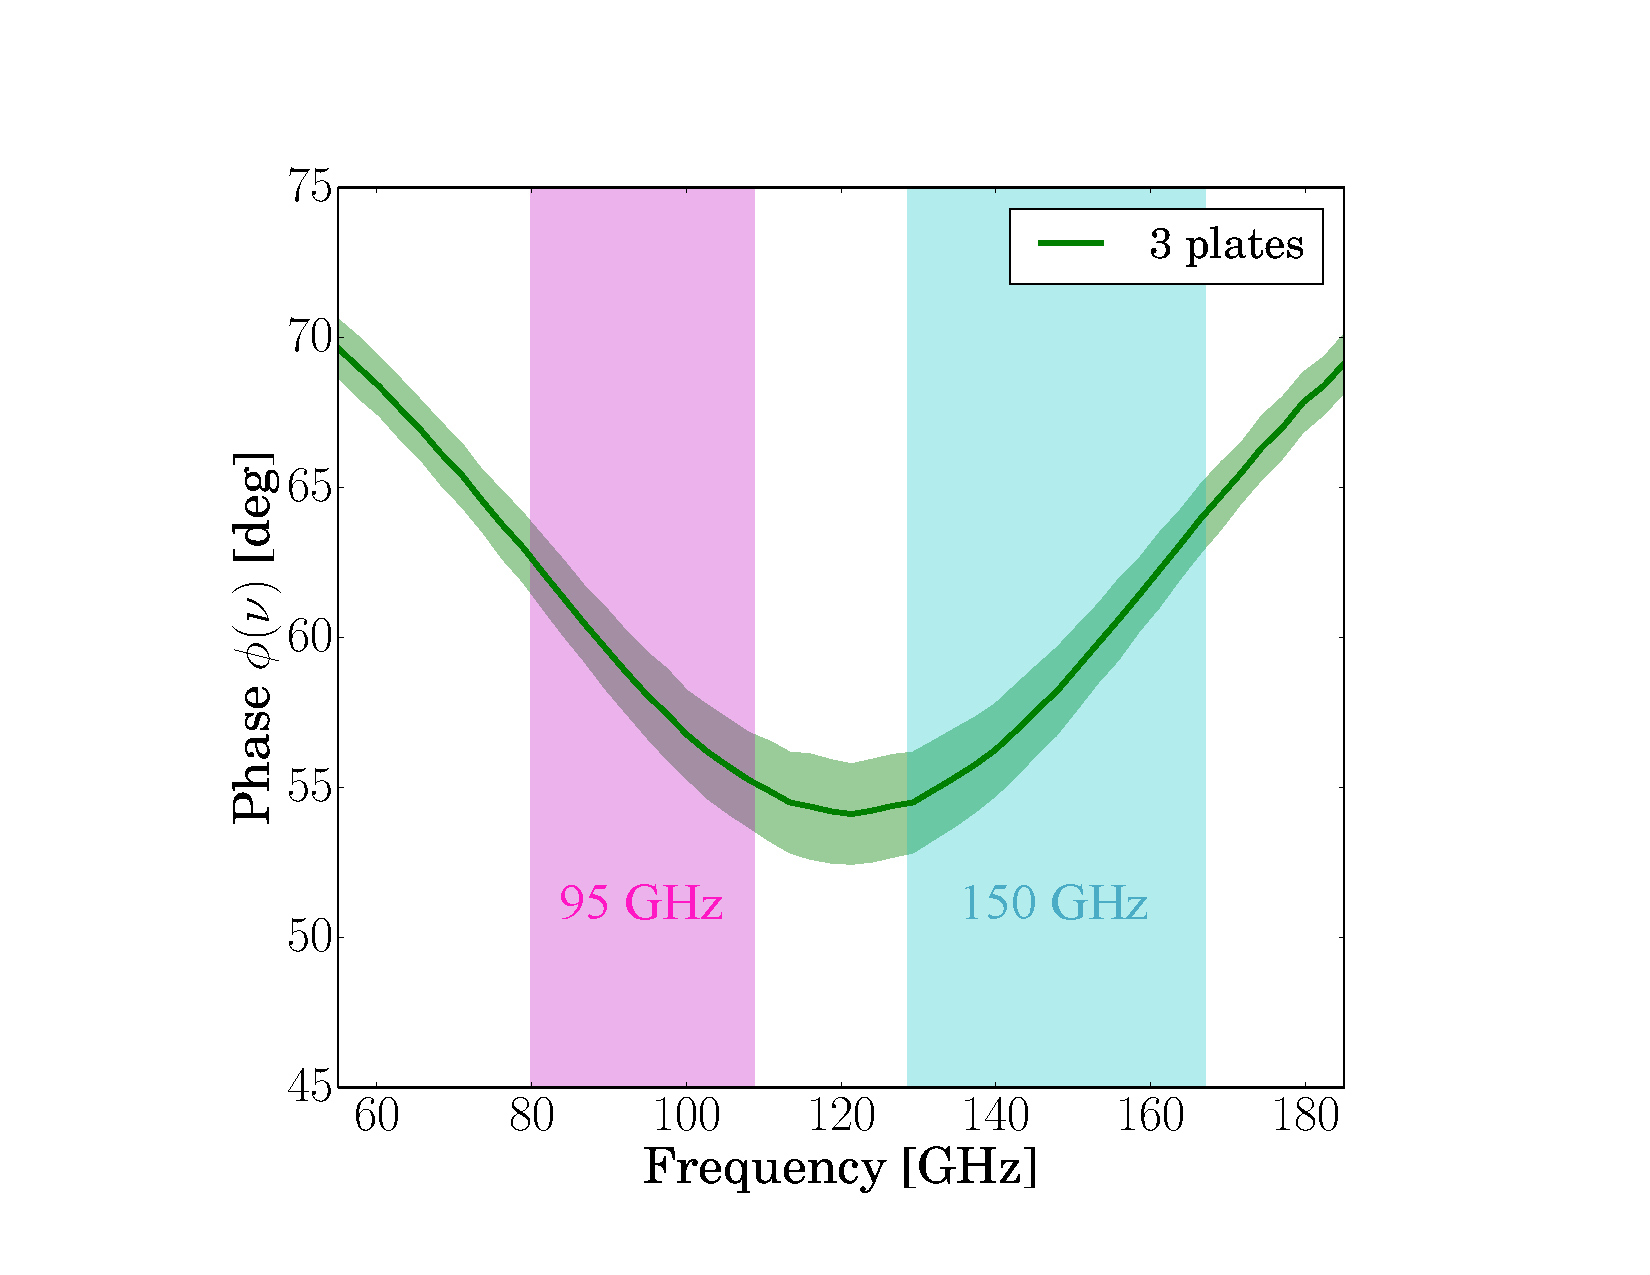
\includegraphics[width=0.48\linewidth, trim=3.5cm 1cm 5cm 2.8cm, clip]{PB2aWHWP/Figures/HWP_Phase.pdf}}
    \vspace{0.2cm}
    \centering
    	\centering
	\begin{tabu}{| c | c | c | c |}
	\hline
	%\multicolumn{4}{|c|}{Measured Stack Performance} \\
	%\hline
	Stack Element & Thickness [mm] & Index of Refraction & Loss Tangent [$\mathrm{10^{-4}}$] \\
	\hline
	\hline
	Top AR Layer: HDPE & $0.38 \pm 0.04$ & $1.55 \pm 0.01$ & $0.5 \pm 1.0$ \\
	\hline
	Bot AR Layer: RO3006 & $0.27 \pm 0.02$ & $2.52 \pm 0.01$ & $56.5 \pm 2.7$ \\
	\hline
	Ordinary Axis & \multirow{2}{*}{$3.75 \pm 0.01$} & $3.05 \pm 0.03$ & $0.1 \pm 1.3$ at 95 GHz \\
	\cline{1-1} \cline{3-3}
	Extraordinary Axis & & $3.38 \pm 0.03$ & $1.1 \pm 1.3$ at 150 GHz \\
	\hline
	\end{tabu}
    \caption[The modulation efficiency and phase for the PB-2a HWP, compared to that of a single-plate HWP.]{Normal-incidence, Mueller matrix calculations of the PB-2a AHWP (green), compared to that of a single-plate HWP (red). The shaded green region represents sapphire-axis measurement and assembly uncertainties, and the magenta and cyan bands show the approximate PB-2a observation bands. Figure~\ref{fig:pb2a_whwp_mod_eff_spectrum:a}  shows modulation efficiency as a function of frequency. The dual-band averaged value 98\%, while that of the single plate is 75\%. Figure~\ref{fig:pb2a_whwp_mod_eff_spectrum:b} shows modulation phase as a function of frequency. That of a single-plate HWP is uniformly zero. \cite{hill_design_2016}. The table shows the measured ambient-temperature thickness, index of refraction, and loss tangent for each layer in the HWP optical stack. Indexes are measured using an FTS (Figure \ref{fig:pb2a_whwp_bandpass}) and loss tangents are measured using a thermal emission apparatus (Figure \ref{fig:pb2a_whwp_sapphire_emission}). The sapphire loss tangent is averaged over the ordinary and extraordinary axes.}
    \label{fig:pb2a_whwp_mod_eff_spectrum}
\end{figure}

%%%%%%%%%%%%%%%%%%%%%%%%%%%%%%%%
%%%%%%%%%%%%%%%%%%%%%%%%%%%%%%%%

\subsection{Sapphire index}
\label{sec:pb2a_whwp_sapphire_index}

In order to both assemble the AHWP for adequate modulation efficiency and measure the sapphire's ordinary and extraordinary refractive indexes, we must first identify the orientation of the crystal axes. Crystal measurements are most commonly done using x-ray diffractometry, but such techniques for PB-2a are precluded by the sapphire's large diameter. Therefore, we leverage the birefringent window's mm-wave polarization properties to identify its axes.\footnote{We need only determine the \textit{relative} orientation of each plate's crystal axes, as opposed to the absolute orientation.}

A schematic of the optical setup is shown in Figure~\ref{fig:pb2a_whwp_sapphire_axis_measurement:a}. A polarized thermal source is coupled and aligned to a broadband polarimeter, and the sapphire window is rotated between them, modulating the detector's output. Detected intensity vs. WHWP angle has two local maxima corresponding to where the ordinary/extraordinary axes align with the source/detector's polarization axes. An example of detected intensity vs. sapphire angle is shown in Figure~\ref{fig:pb2a_whwp_sapphire_axis_measurement:b}. In this particular test, data is collected over a span of $20^{\circ}$ and is fit to a parabola to constrain the maximum to $< 0.5^{\circ}$. Including uncertainties in the polarization leakage of the input and output wire grids, the relative alignment between the source and detector axes, the accuracy with which the axes are marked, and the precision with which the stack is assembled, the relative alignment between the plates' crystal axes $< 1.1^{\circ}$. This axis-orientation uncertainty drives the uncertainty of the expected modulation efficiency and phase, which are represented as shaded bands in Figure~\ref{fig:pb2a_whwp_mod_eff_spectrum} and are small enough to maintain $> 95$\% polarization efficiency across the PB-2a bands.

\begin{figure}[!t]
    \centering
    \subfloat[\label{fig:pb2a_whwp_sapphire_axis_measurement:a}]{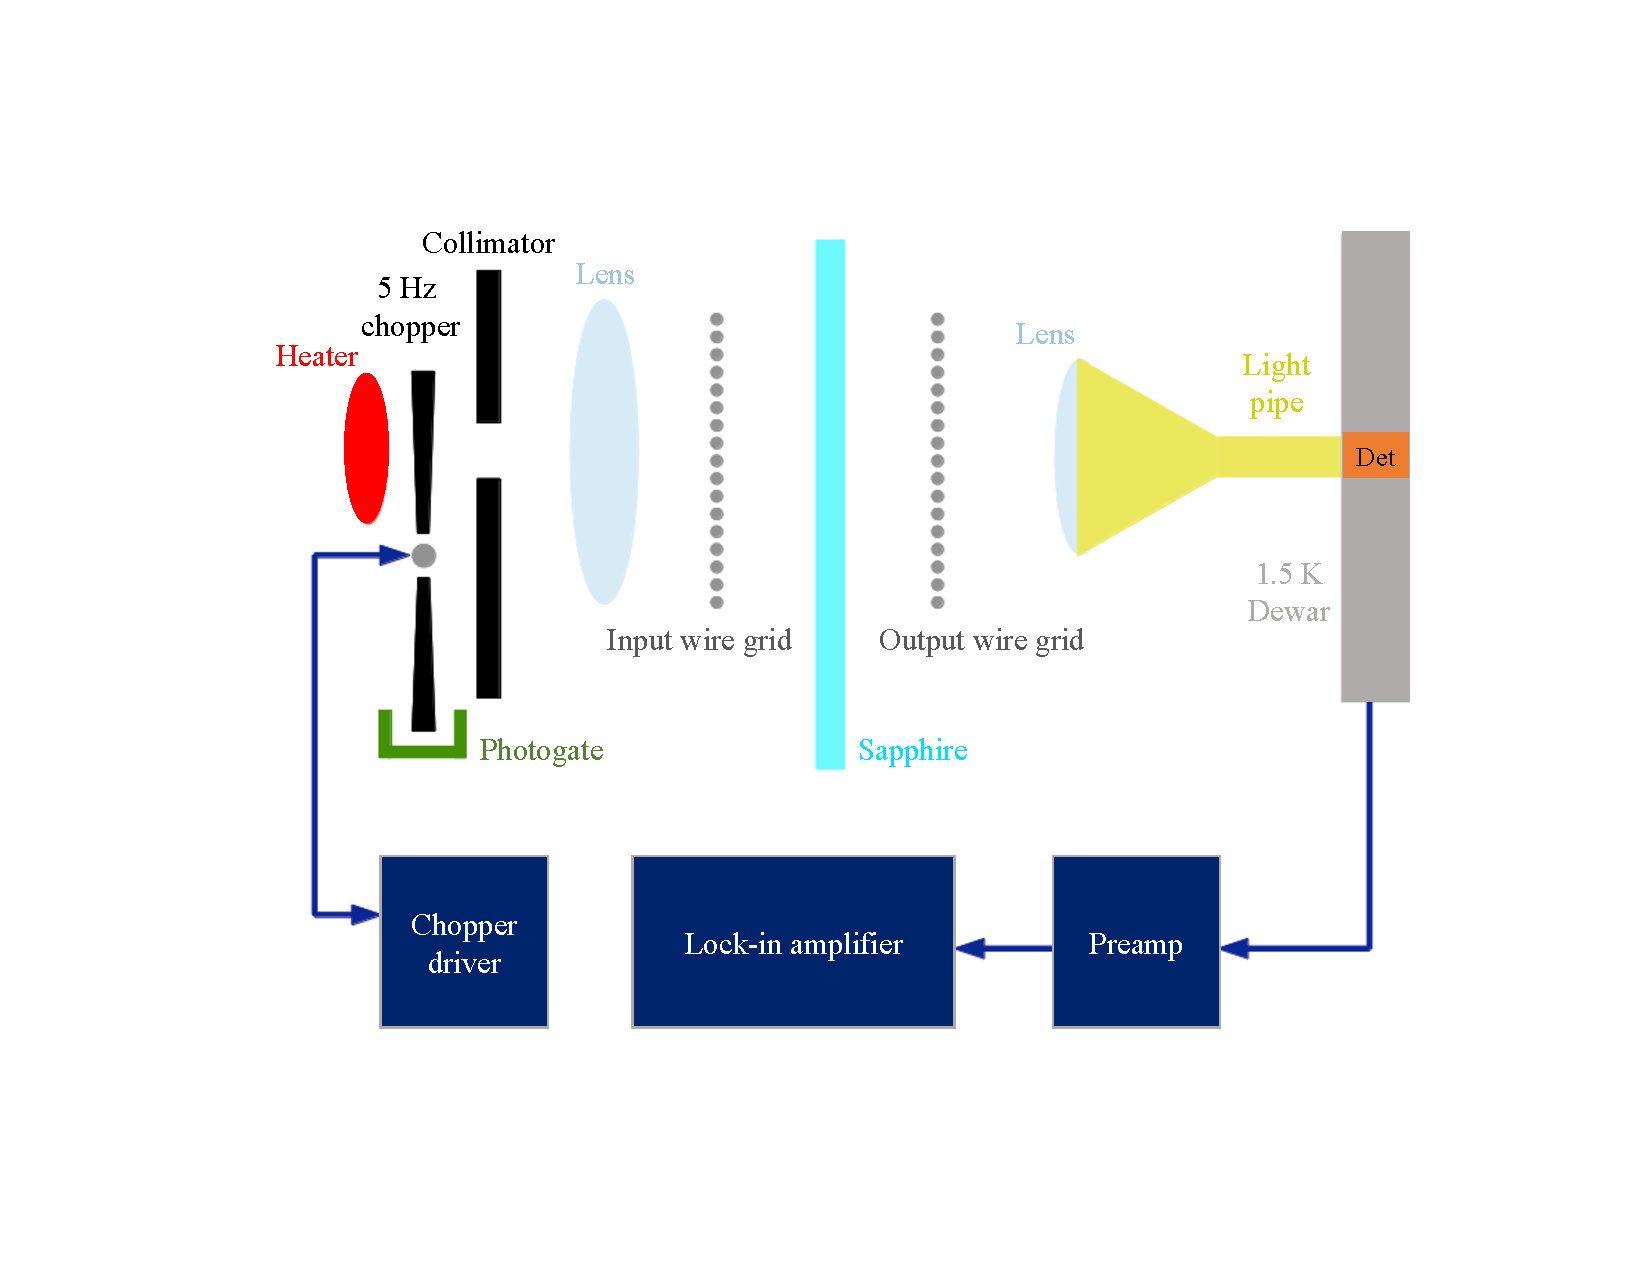
\includegraphics[width=0.48\linewidth, trim=4cm 3cm 3cm 3cm, clip]{PB2aWHWP/Figures/sapphire_axis_apparatus.pdf}}
    \subfloat[\label{fig:pb2a_whwp_sapphire_axis_measurement:b}]{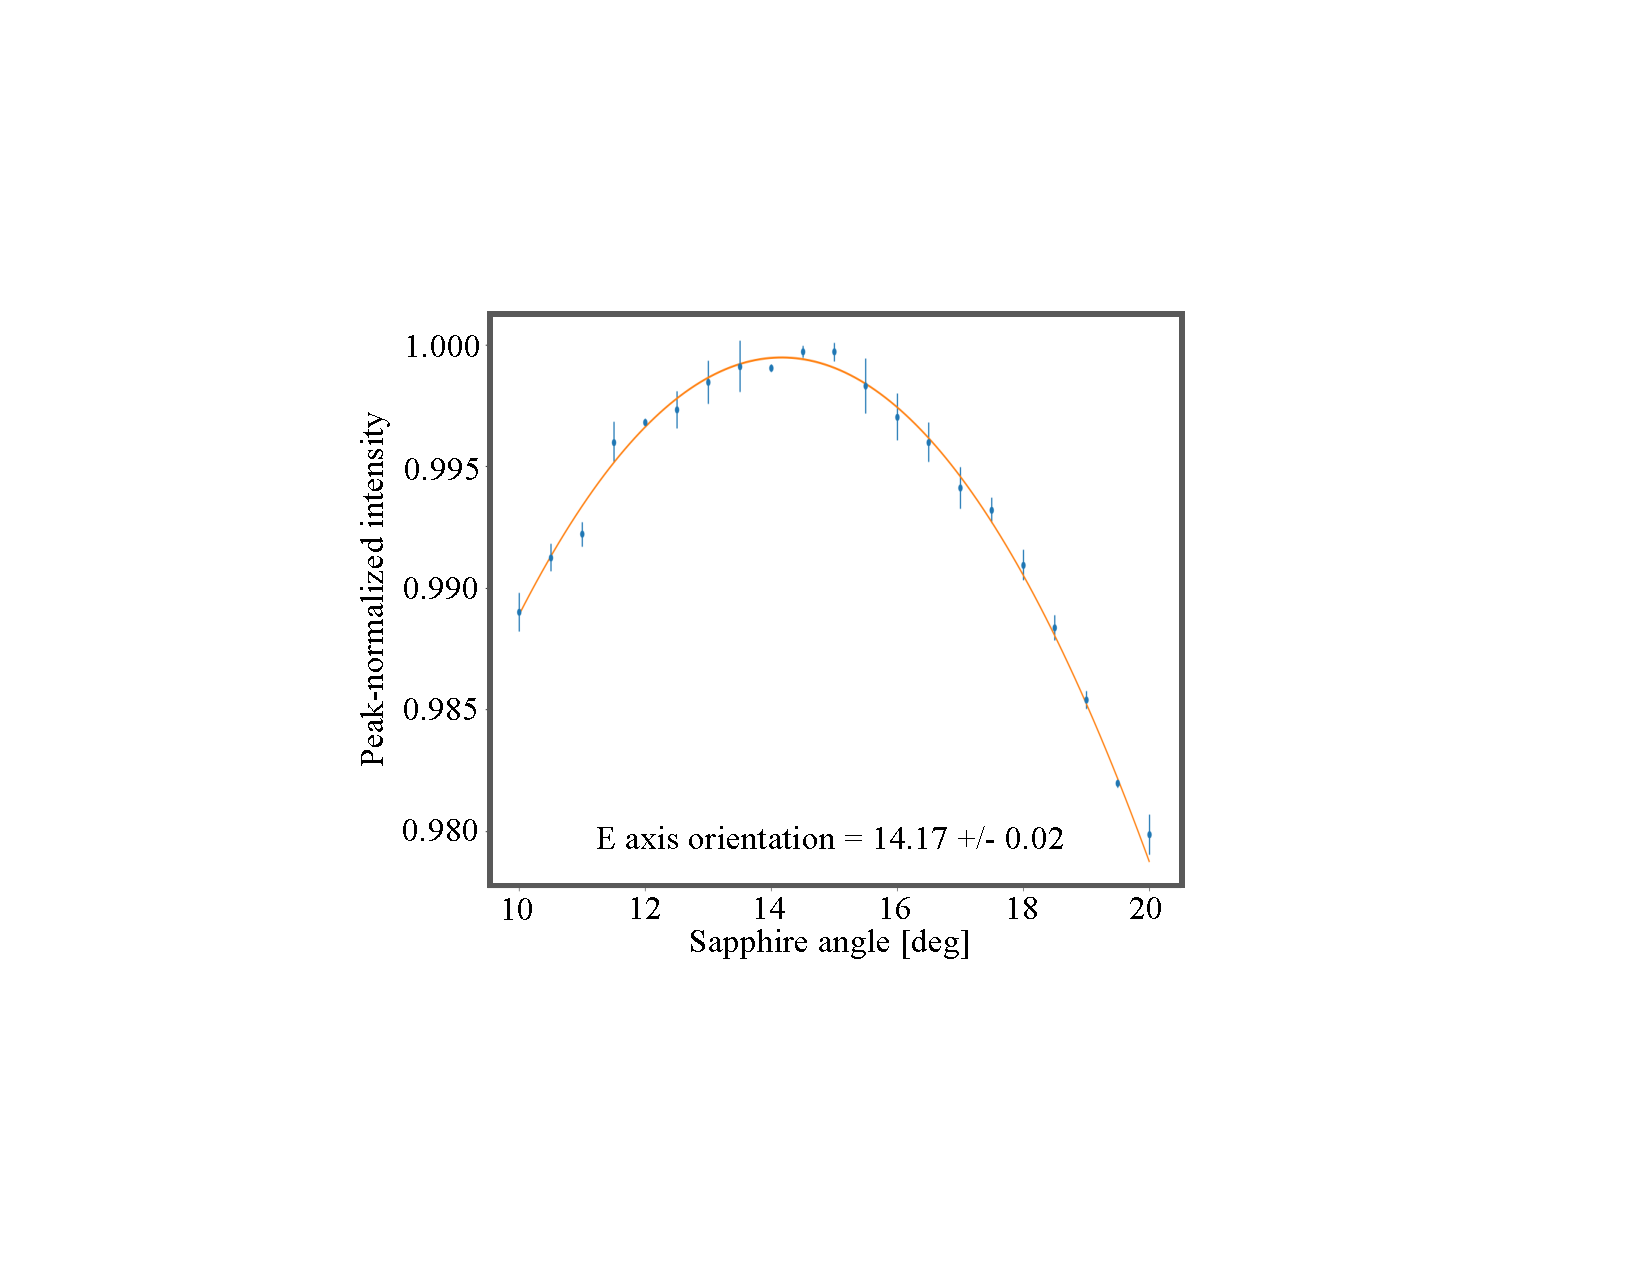
\includegraphics[width=0.48\linewidth, trim=6cm 6cm 7cm 5cm, clip]{PB2aWHWP/Figures/sapphire_axis_measurement.pdf}}
    \caption[PB-2a sapphire crystal axis orientation measurement]{PB-2a sapphire crystal axis orientation measurement. The measurement apparatus is shown in Figure~\ref{fig:pb2a_whwp_sapphire_axis_measurement:a}. A $\sim$~$700^{\circ}$ C ceramic thermal source is chopped at $\approx$~20~Hz and collimated by an absorbing screen. A lens focuses the collimated beam through a wire grid onto the sapphire plate, for which the output is polarized using another wire grid, is collimated using a lens and light pipe, and is detected by a neutron transmutation doped (NTD) Germanium bolometer at $\approx$~1.5~K. Detector output vs. WHWP angle is shown in Figure~\ref{fig:pb2a_whwp_sapphire_axis_measurement:b}, and the maximum corresponds to the ordinary/extraordinary axis location. This orientation is then marked and used to align the Pancharatnam stack.}
    \label{fig:pb2a_whwp_sapphire_axis_measurement}
\end{figure}

In addition to identifying the orientation of the sapphire's crystal axes, we measure each piece's ordinary and extraordinary refractive indexes. We use the FTS system shown in Figure~\ref{fig:pb2a_whwp_bandpass:a} except with two aligned wire grid polarizers on either side of the sapphire window, which allows us to isolate each crystal axis. The measured Fabry-P\'{e}rot fringe pattern is then fit to extract the indexes, which are shown in the table of Figure~\ref{fig:pb2a_whwp_mod_eff_spectrum}. While attenuation estimates are also extracted from FTS sapphire data, the sapphire loss tangent is so small and the windows so thin that constraining $\tan \delta$ meaningfully is difficult. Nonetheless, a proper estimate of the sapphire loss is critical to evaluating the WHWP's emissivity, and therefore we perform a dedicated measurement of the sapphire loss, as described in Section~\ref{sec:pb2a_whwp_sapphire_loss}.

%%%%%%%%%%%%%%%%%%%%%%%%%%%%%%%%
%%%%%%%%%%%%%%%%%%%%%%%%%%%%%%%%

\subsection{Sapphire loss}
\label{sec:pb2a_whwp_sapphire_loss}

PB-2a mapping speed is quite sensitive to WHWP emissivity, as shown in Figure~\ref{fig:pb2a_whwp_emissivity_reflectivity_mappingSpeed}, and WHWP emissivity is in turn quite sensitive to dielectric loss in the sapphire. Therefore, a precise measurement of sapphire loss tangent $\tan \delta$ in the PB-2a frequency range is critical to the HWP design process. See Section~\ref{sec:sensitivity_emissivity} for a discussion of dielectric loss. 

Sapphire is expected to have $\tan \delta \sim 10^{-4}$ at 150~GHz (cite lamb) and 300~K, making an emissivity measurement of 3.75~mm-thick windows challenging.\footnote{CMB optical engineers often test small before purchasing the deployable optic. However, sapphire quality is sensitive to the properties of its specific growth, and it is expensive to purchase small pieces from growths intended for large-diameter slabs. Therefore, we choose to measure and ``certify'' the 512~mm-diameter, 3.75~mm-thick pieces that comprise the deployment-ready HWP instrument.} To meet this challenge, we construct the thermal emission apparatus (TEA) shown schematically in Figure~\ref{fig:pb2a_whwp_sapphire_emission}.

\begin{figure}[!t]
    \centering
    \subfloat[\label{fig:pb2a_whwp_sapphire_emission:a}]{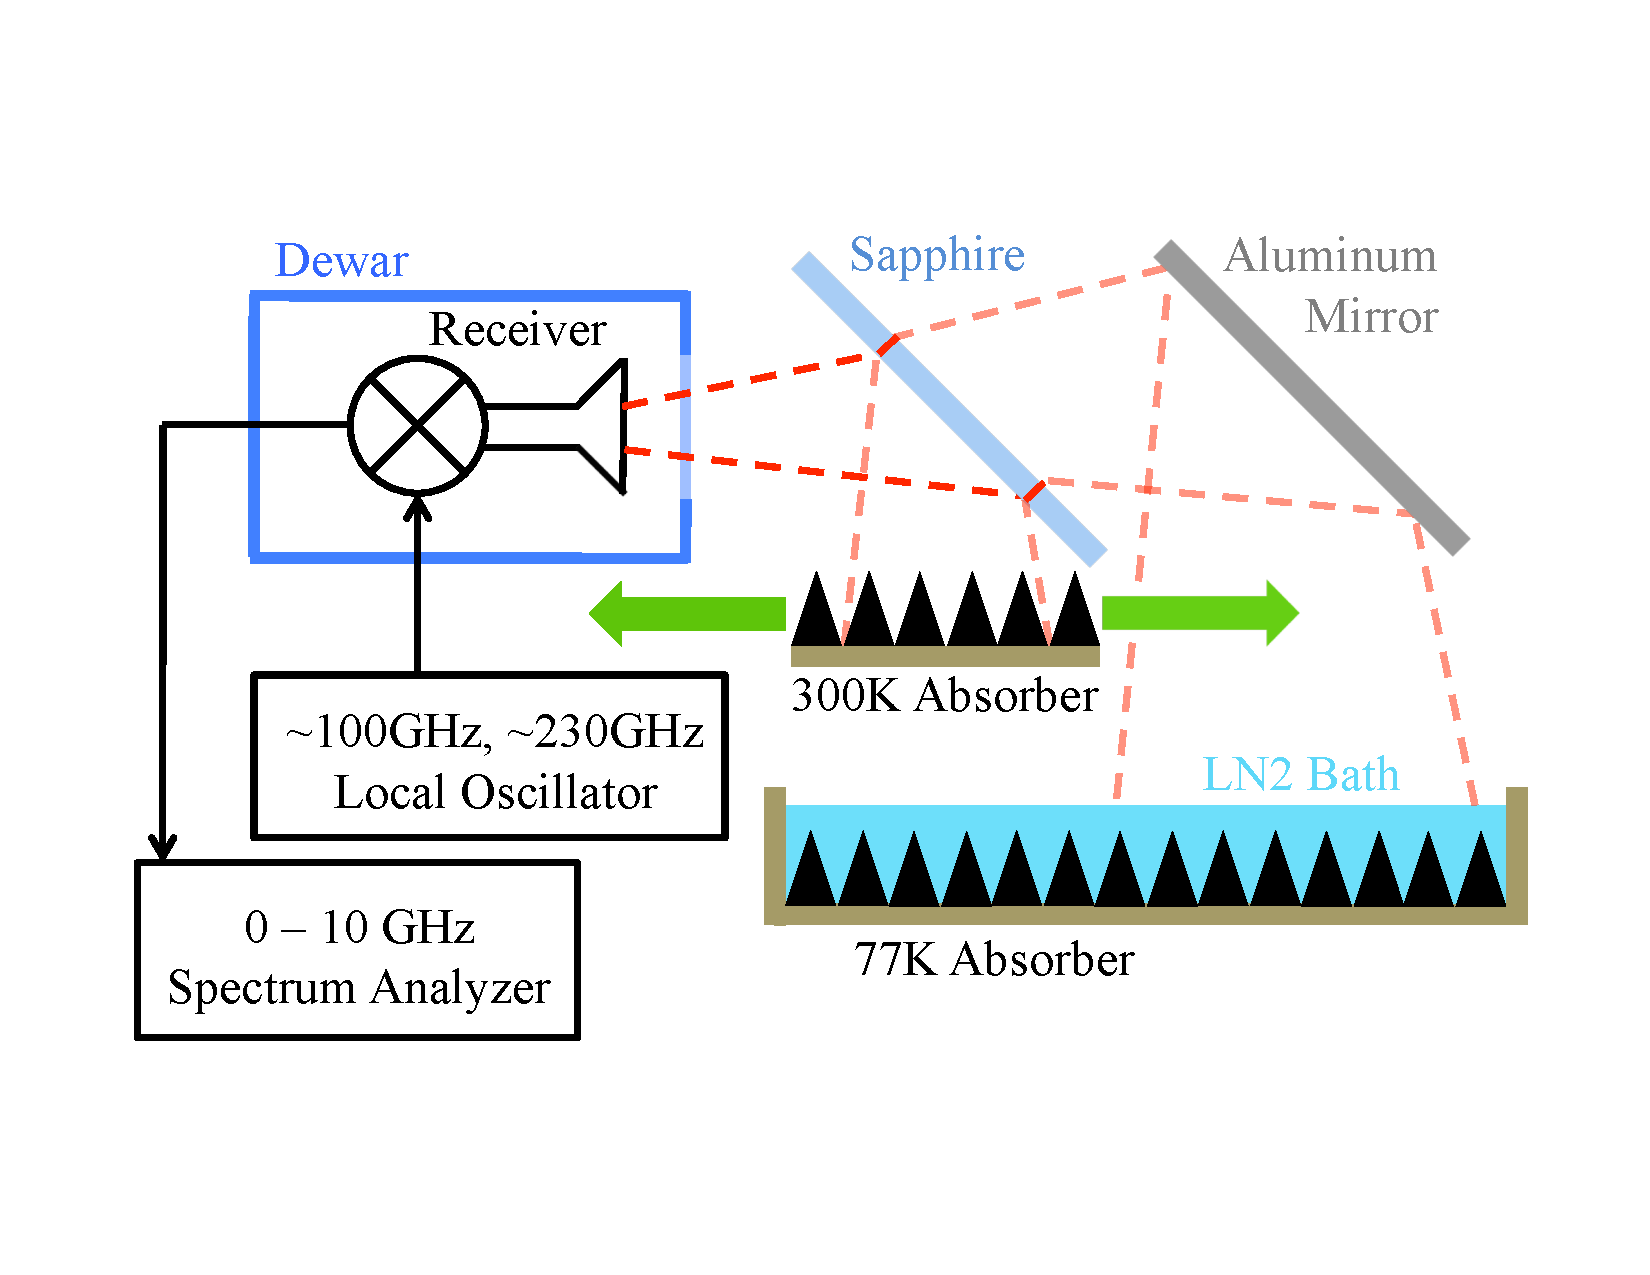
\includegraphics[width=0.48\linewidth, trim=2cm -1.5cm 0cm 4cm, clip]{PB2aWHWP/Figures/TEA.pdf}}
    \subfloat[\label{fig:pb2a_whwp_sapphire_emission:b}]{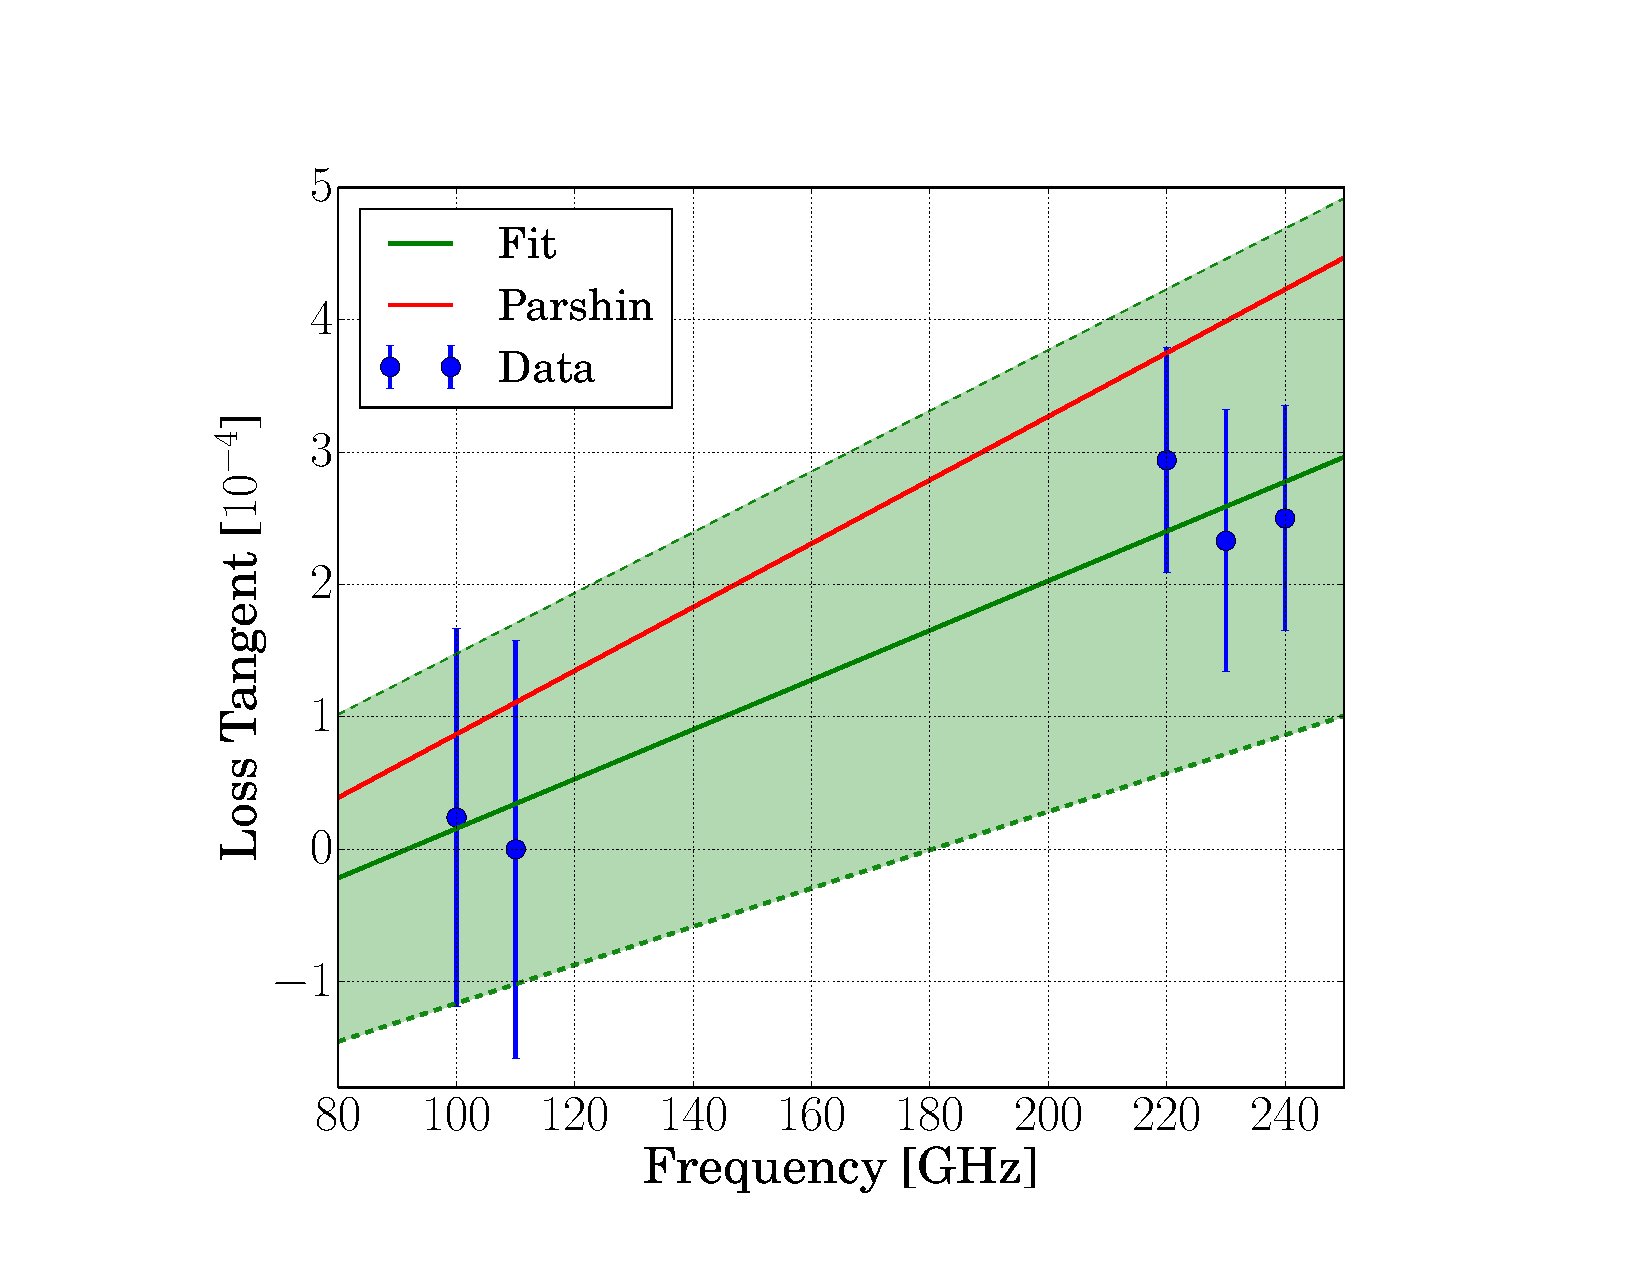
\includegraphics[width=0.48\linewidth, trim=3cm 1cm 6cm 4cm]{PB2aWHWP/Figures/SapphireLoss.pdf}}
    \vspace{0.2cm}
    \centering
	\begin{tabu}{| c | c | c | c |}
	\hline
	Sapphire & Reflected & Transmitted & Purpose \\
	\hline
	\hline
	- & - & 77 K & Calibrate receiver noise temp \\
	\hline
	- & - & 300 K & Calibrate receiver gain \\	
	\hline
	Y & 300 K & 77 K & Calibrate reflection \\	
	\hline
	Y & 77 K & 300 K & Calibrate transmission \\ 
	\hline
	Y & 77 K & 77 K & Measure emission \\
	\hline
	\end{tabu}
    \caption[Sapphire warm loss tangent measurement]{Sapphire warm loss tangent measurement. Figure~\ref{fig:pb2a_whwp_sapphire_emission:a} shows the apparatus used to measure the sapphire loss at room temperature. Thermal emission from the sapphire slab is measured over a 77 K background using a heterodyne receiver. A series of configurations involving 300 K absorber are used to calibrate receiver gain, receiver noise, reflection from the sapphire, and transmission through the sapphire. Figure~\ref{fig:pb2a_whwp_sapphire_emission:b} shows a measurement of the IF-band-averaged, axes-averaged GHTOT sapphire tan $\delta$ at 5 LO frequencies with error bars that account for both statistical and systematic uncertainty (blue points), a linear fit to those data points (green band), and data presented in Parshin et al. (red line) \cite{parshin_silicon_1995}. The table shows the TEA configurations used to characterize the sapphire loss. The first column shows whether the sapphire is present, the second which temperature the sapphire reflects to, the third which temperature the mirror reflects to, and the fourth the configuration's purpose. \label{fig:pb2a_whwp_sapphire_emission}}
\end{figure}

The TEA measures the temperature increase over a 77 K background due to thermal emission from a dielectric slab. We use a 100 GHz/300 GHz heterodyne receiver previously used on the Combined Array for Research in Millimeter-wave Astronomy (CARMA). The receiver features horn-coupled SIS (superconducting-insulating-superconducting) mixers cooled to 4 K, fed by a tunable local oscillator (LO) to produce a 1-10 GHz intermediate-frequency (IF) band that is digitized with a spectrum analyzer. 

Because the sapphire is not AR coated during this evaluation, it is important that radiation reflected from the slab's front surface terminates on 77 K. Thus, as shown in Figure~\ref{fig:pb2a_whwp_sapphire_emission:a}, the sapphire is mounted at a 45-degree angle to the receiver in front of an aluminum sheet ($\lesssim$~1~$\mathrm{\mu m}$ RMS surface roughness) also mounted at 45 degrees. Both the sapphire and the mirror reflect to pyramidal absorber submerged in a liquid nitrogen bath. The sapphire is on a rotating stage, and the receiver is optimized for p-polarization, so as to maximize signal transmission through the slab. Measurements were made at LO frequencies of 100, 110, 220, 230, and 240 GHz. At each frequency we made a series of five measurements listed in the table of Figure~\ref{fig:pb2a_whwp_sapphire_emission} in order to solve for the receiver noise temperature and gain as well as the sapphire reflection coefficient, transmission coefficient, and emissivity.

Several factors complicate the calculation of tan $\delta$. First, the sapphire slab acts as a Fabry-Per\'{o}t etalon, creating a series of transmission peaks with $\approx$~13 GHz spacing. Absorption, and hence thermal emission, in the slab is maximized at these frequencies and minimized at the reflection peaks between them. Second, measuring this pattern is complicated by the double sideband receiver, which folds signals above and below the LO frequency into a single IF band. Finally, the principle axes of the sapphire were not accurately known at the time of these measurements. Simulations based on analytic techniques \cite{essinger-hileman_transfer_2013} (cite Hou too) show that averaging the data across the IF band and over a range of sapphire azimuth angles incurs systematic error that is smaller than the noise in our measurement. Therefore, we present the band-averaged, sapphire-angle-averaged tan $\delta$ values in Figure \ref{fig:pb2a_whwp_sapphire_emission:b}. The measured GHTOT sapphire $\tan \delta$ is consistent with the literature value \cite{parshin} to within our 1$\sigma$ uncertainty of $\approx 10^{-4}$.

To estimate the sapphire tan $\delta$ in the PB2 frequency bands, we linearly interpolate the measured $\tan \delta$ to the 90/150~GHz bands, and the resulting values are given in the table of Figure~\ref{fig:pb2a_whwp_mod_eff_spectrum}. We find that the in-band sapphire absorptivity is smaller than in the RO3006 AR layers, and therefore, the GHTOT sapphire suits PB-2a's needs.

%%%%%%%%%%%%%%%%%%%%%%%%%%%%%%%%
%%%%%%%%%%%%%%%%%%%%%%%%%%%%%%%%

\subsection{Transmissivity}
\label{sec:pb2a_whwp_transmissivity}

To validate the HWP AR performance, we utilize an FTS coupled to a broadband detector, as shown schematically in Figure \ref{fig:pb2a_whwp_bandpass:a}. Signal from a temperature-modulated source is collimated by an off-axis parabolic mirror. This beam travels through the WHWP, is split between a pistoned and fixed path by a 250-$\mu$m-thick Mylar film, is recombined by the same splitter, and focuses onto a 0.3~K bolometer via an ultra-high-molecular-weight polyethylene (UHMWPE) collimator lens. The detector output is sent to a lock-in amplifier whose value is integrated for 0.5 s at each moving-mirror position. The mirror step size and dynamic range give a 1 GHz resolution over a 300 GHz bandwidth.

\begin{figure}[!t]
    \centering
    \subfloat[\label{fig:pb2a_whwp_bandpass:a}]{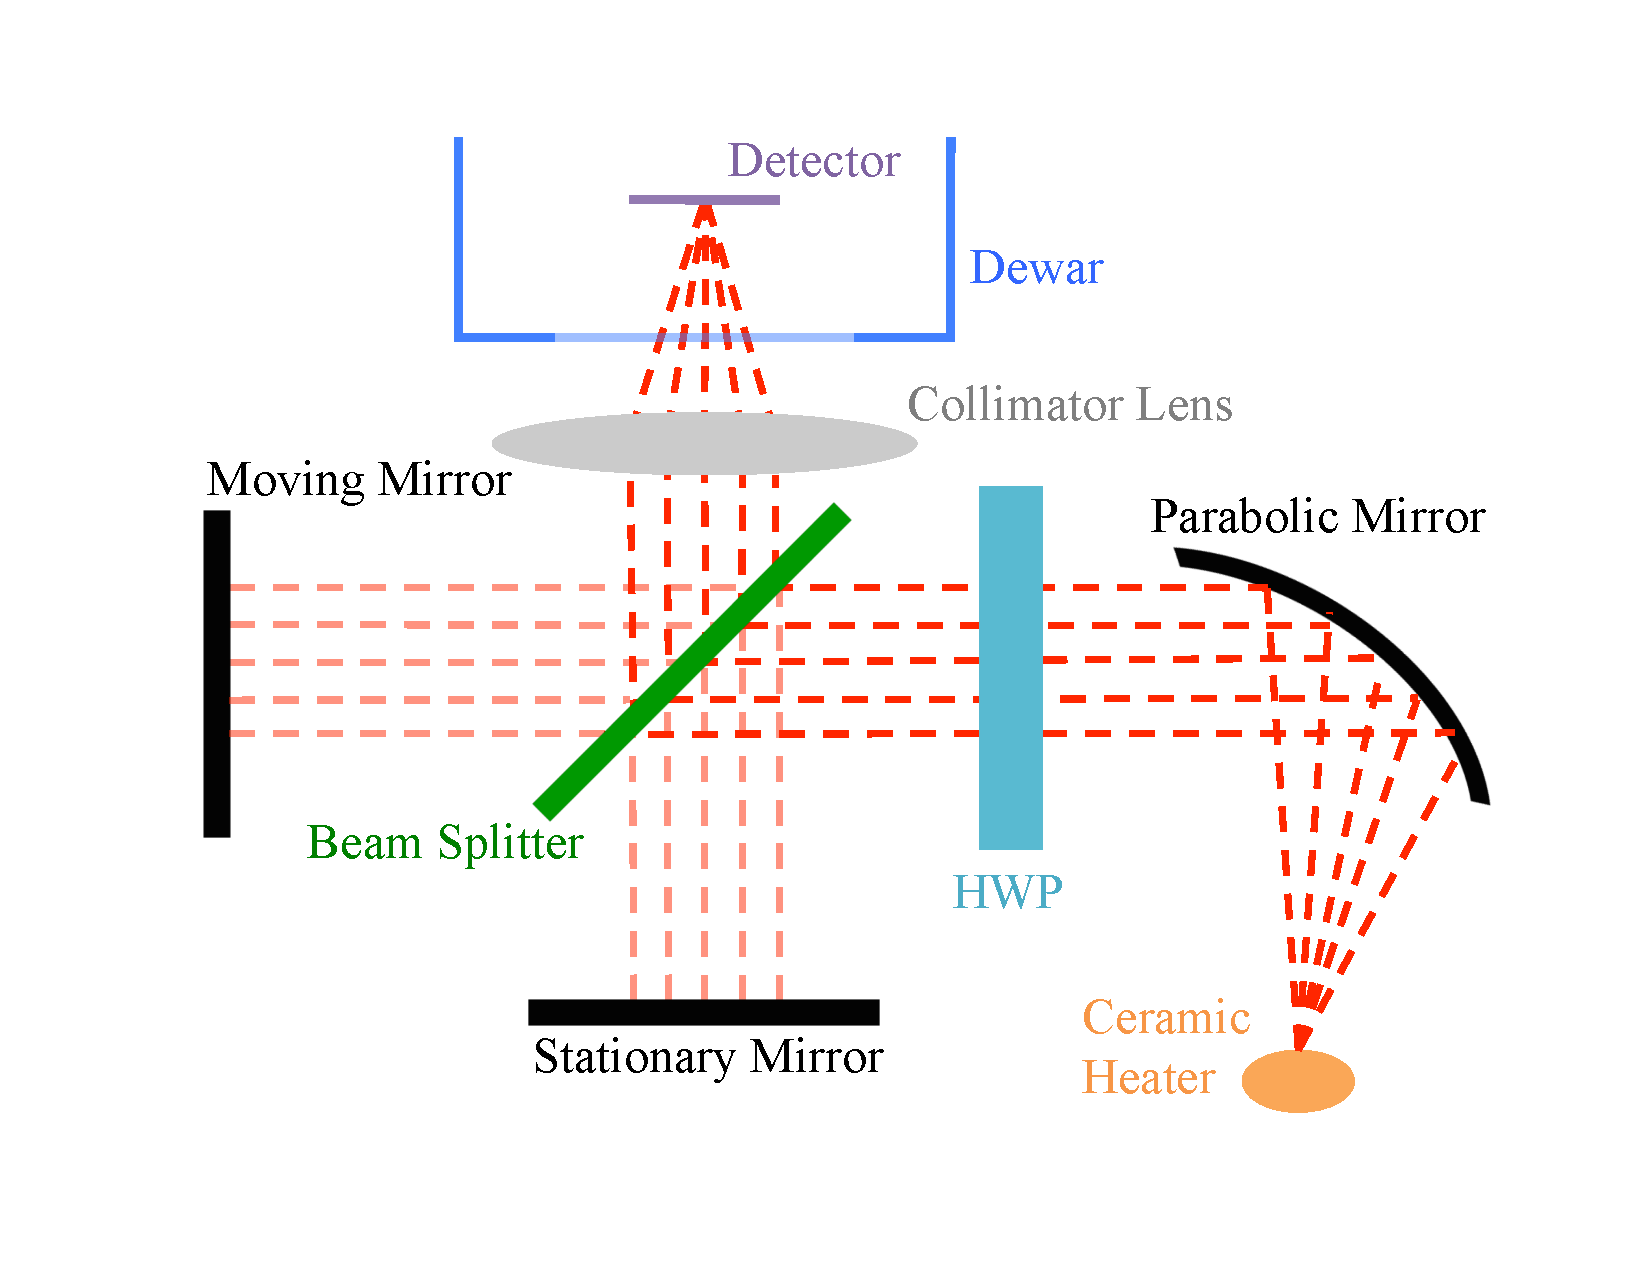
\includegraphics[width=0.48\linewidth, trim=3cm 0.5cm 2cm 2cm, clip]{PB2aWHWP/Figures/FTSCartoon.pdf}}
    \subfloat[\label{fig:pb2a_whwp_bandpass:b}]{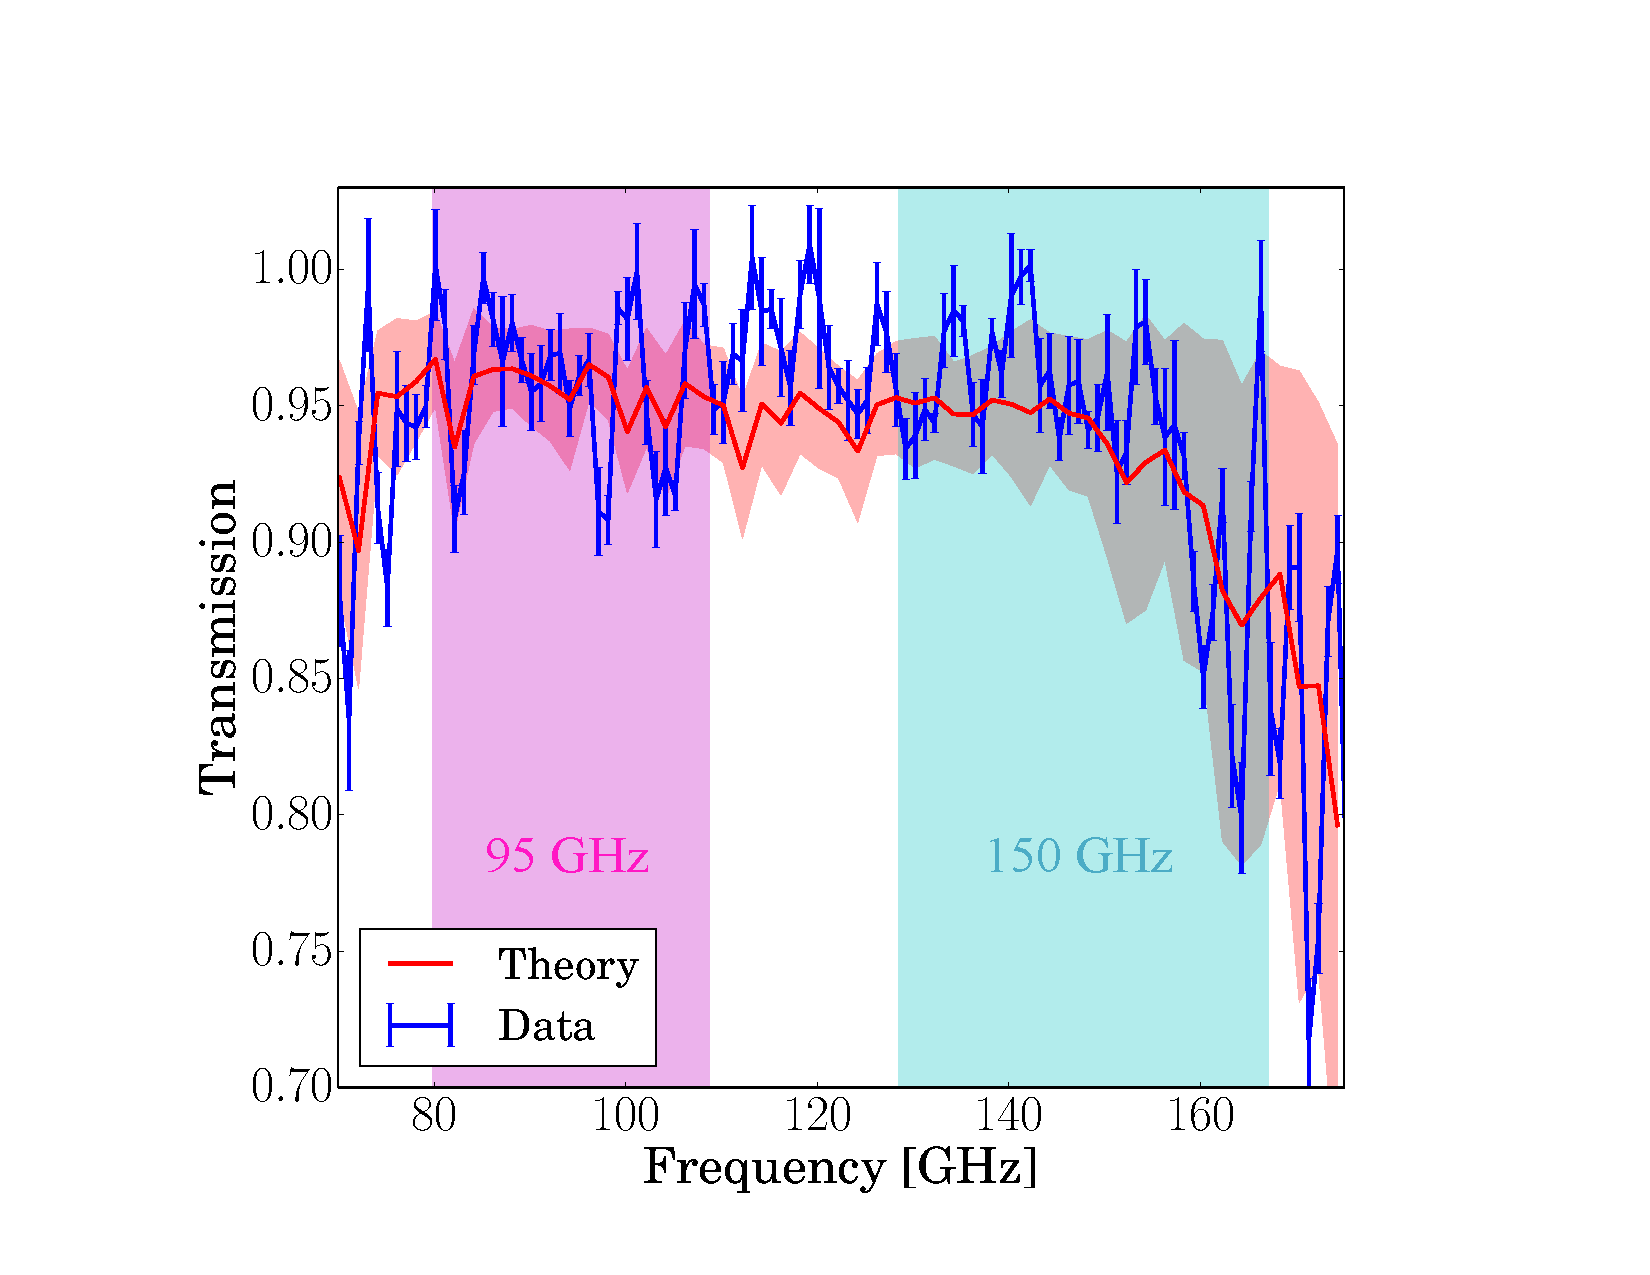
\includegraphics[width=0.48\linewidth, trim=2cm 1cm 5cm 3cm, clip]{PB2aWHWP/Figures/HWPBandpass.pdf}}
    \vspace{0.2cm}
    \centering
    \begin{tabu}{| c | c | c |}
	\hline
	%\multicolumn{3}{|c|}{Measured AHWP Intensity Performance} \\
	%\hline
	Band & Transmissivity & Emissivity \\
	\hline
	\hline
	95 GHz & $0.959 \pm 0.014$ & $0.020 \pm 0.009$ \\
	\hline
	150 GHz & $0.941 \pm 0.015$ & $0.032 \pm 0.014$  \\
	\hline
	\end{tabu}
    \caption[A schematic of the FTS apparatus and resulting PB-2a WHWP bandpass.]{Figure~\ref{fig:pb2a_whwp_bandpass:a} shows a cartoon of the FTS apparatus used to
    measure the WHWP transmissivity. Signal from a temperature-modulated source is collimated, travels through the optical stack into the FTS, and is focused onto a 0.3~K bolometer. Figure~\ref{fig:pb2a_whwp_bandpass:b} shows the measured transmission for the PB-2a WHWP between 60 and 180 GHz using the FTS. The blue points represent the measured HWP-angle-averaged transmissivity. The red line and shaded region represent the theoretical expectation using a transfer matrix calculator \cite{essinger-hileman_transfer_2013} and the individual-layer measurements shown in the table of Figure~\ref{fig:modulation_effciency_countors}. The measured bandpass agrees with the expectation to within 1~$\sigma$. The table presents the band-integrated transmissivity and emissivity across each PB-2a frequency channel.}
    \label{fig:pb2a_whwp_bandpass}
\end{figure}

We repeat the described process with the WHWP removed in order to divide out any spectral affects of the FTS setup and normalize the transmissivity. Additionally, we repeat the measurement at various HWP azimuth positions to average over any polarization of the ceramic source induced by the chopper blade or the input mirror.

The result of the FTS measurement is shown by the ``Data'' curve in Figure \ref{fig:pb2a_whwp_bandpass:b}. We integrate the measured transmission across each PB-2a frequency band to obtain the 90/150~GHz HWP transmission values in the table of Figure~\ref{fig:pb2a_whwp_bandpass}. To estimate the emissivity, we simulate~\cite{essinger-hileman_transfer_2013} HWP transmission vs. frequency using the dielectric layer parameters in the table of Figure~\ref{fig:pb2a_whwp_mod_eff_spectrum} and isolate the loss due to absorption. The result of the transmission simulation is shown by the theory curve in Figure~\ref{fig:pb2a_whwp_bandpass:b}, and the simulated transmission is consistent with the measured transmission to within 1~$\sigma$.

%%%%%%%%%%%%%%%%%%%%%%%%%%%%%%%%
%%%%%%%%%%%%%%%%%%%%%%%%%%%%%%%%

\subsection{Polarization efficiency}
\label{sec:pb2a_whwp_polarization_efficiency}

To measure the HWP polarization modulation efficiency, we utilize the setup shown schematically in Figure~\ref{fig:pb2a_whwp_polarization_efficiency:a}. Signal from a chopped thermal source is polarized with a wire grid, and the grid is tilted to avoid standing waves between it and the chopper. The polarized beam travels through the WHWP, is polarized by another wire grid, and is focused by an UHMWPE collimator lens onto PB-2a-style 90~and 150~GHz detectors. Even though the sinuous antenna is polarized, we introduce a wire grid on the detector-side of the HWP to mitigate any frequency-dependent polarization angles~(cite Jen Edwards). The WHWP angle is stepped in $10^{\circ}$ increments and the detector output is sent to a lock-in amplifier whose value is integrated for 1.0 s at each HWP orientation.

\begin{figure}[!t]
    \centering
    \subfloat[\label{fig:pb2a_whwp_polarization_efficiency:a}]{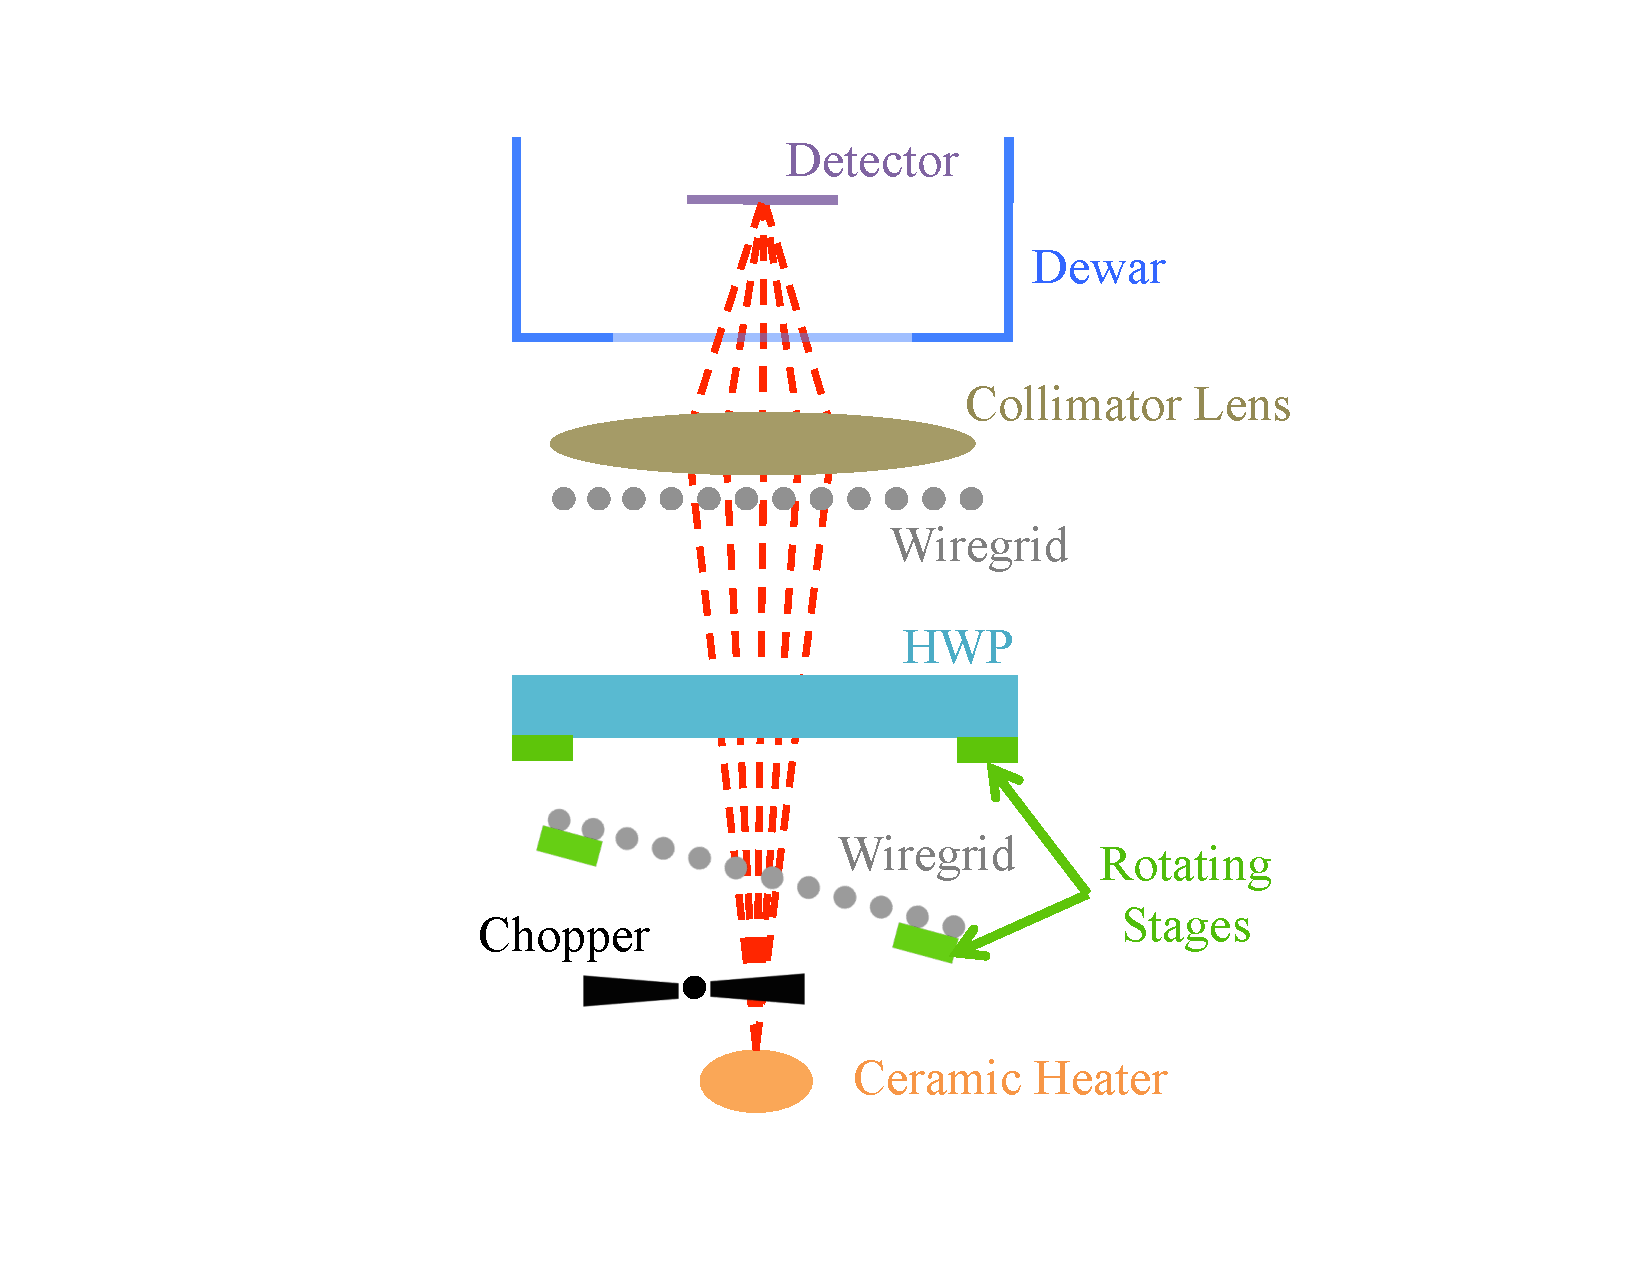
\includegraphics[width=0.48\linewidth, trim=5cm 2cm 4cm 2cm]{PB2aWHWP/Figures/PolModCartoon.pdf}}
    \subfloat[\label{fig:pb2a_whwp_polarization_efficiency:b}]{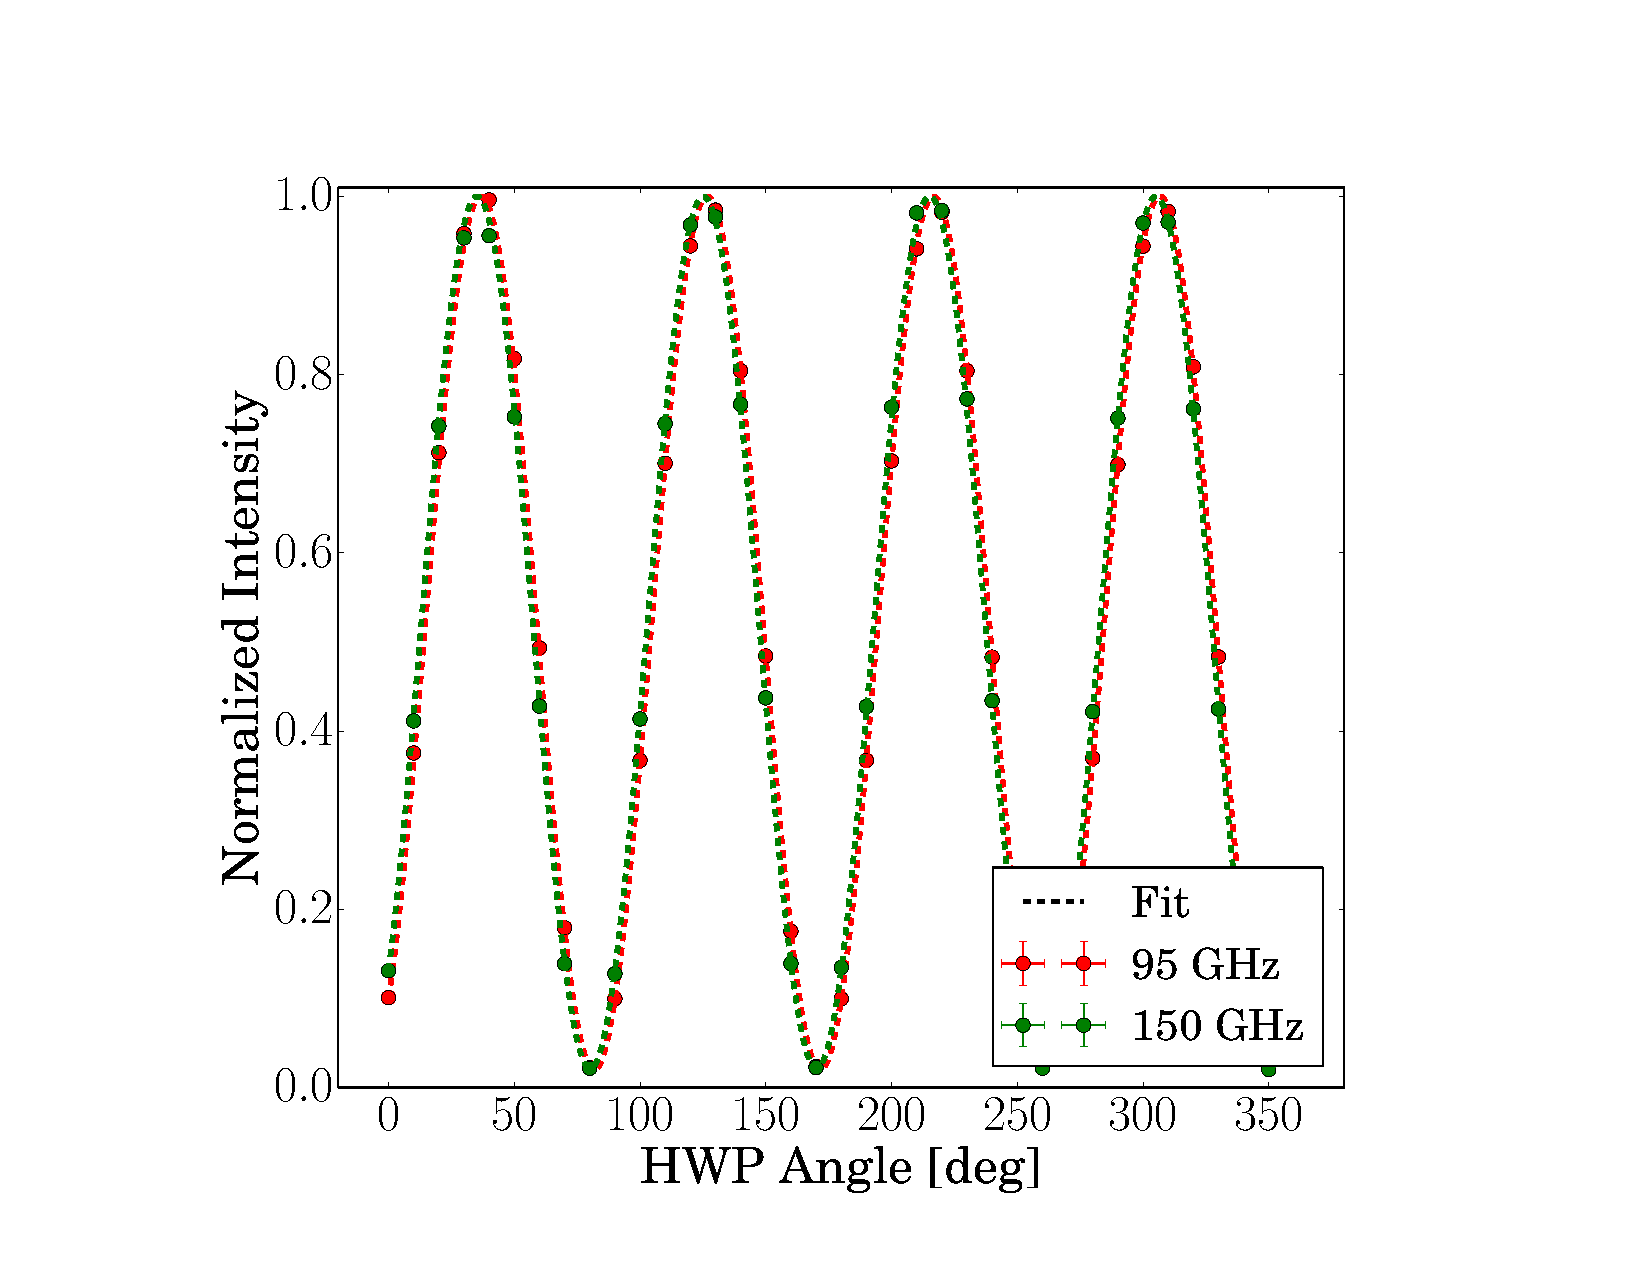
\includegraphics[width=0.48\linewidth, trim=3.5cm 1cm 5cm 3cm, clip]{PB2aWHWP/Figures/polMod.pdf}}
    \vspace{0.2cm}
    \centering
    \begin{tabu}{| c | c | c |}
	\hline
	Band & Modulation Efficiency & Phase Difference \\
	\hline
	\hline
	90 GHz & $0.989 \pm 0.005$ & \multirow{2}{*}{$1.3 \pm 0.1$ deg} \\
	\cline{1-2}
	150 GHz & $0.984 \pm 0.004$ &  \\
	\hline
	\end{tabu}
    \caption[Measurement of the PB-2a WHWP polarization modulation efficiency in the PB2a observation bands]{Measurement of the PB-2a WHWP polarization modulation efficiency in the PB2a observation bands. \ref{fig:pb2a_whwp_polarization_efficiency:a} a shows a cartoon of the polarized measurement apparatus. The HWP is mounted on a rotating stage to modulate a polarized thermal source with respect to a polarized detector. \ref{fig:pb2a_whwp_polarization_efficiency:b} shows normalized intensity as a function of HWP angle in each PB2 frequency band. The points are the data and the dotted lines are the fits to Equation 4. The 95 GHz modulation (in red) is slightly ahead of the 150 GHz modulation (in green). The error bars for the measured data points are small and hence are hidden in this plot. The table presents the band-integrated modulation efficiency across and phase difference between the PB-2a observation bands.}
    \label{fig:pb2a_whwp_polarization_efficiency}
\end{figure}

The results of the modulation efficiency measurement is shown in Figure~\ref{fig:pb2a_whwp_polarization_efficiency:b} with a fit to
\begin{equation}
	S_{\mathrm{det}} = \varepsilon \, \cos^{2}\Big[2 (\chi - \phi)\Big] + (1 - \varepsilon) \, ,
\label{eq:fitPol}
\end{equation} 
where $S_{\mathrm{det}}$ is the normalized signal seen by the detector, $\chi$ is the WHWP angle, $\phi$ is the HWP modulation phase (see Equation~\ref{eq:modulation_phase_function}), and $\varepsilon$ is the modulation efficiency (see Equation~\ref{eq:linear_polarization_modulation_efficiency}). To characterize the cross polarization inherent to the setup, we remove the HWP and step the azimuthal angle of the tilted wire grid in 10-degree increments over a 180-degree range. We fit this data to a model given by
\begin{equation}
	S_{\mathrm{det}} = (1 - L) \, \sin^{2}\Big[\rho_{\mathrm{WG}} - \phi_{\mathrm{WG}}\Big] + L \, ,
\label{eq:wg}
\end{equation} 
where $S_{\mathrm{det}}$ is the normalized signal seen by the detector, $\rho_{\mathrm{WG}}$ is the wire grid azimuthal angle, $\phi_{\mathrm{WG}}$ is some phase, and $L$ is the wire grid polarization leakage. We find the leakage of the setup to be $<$ 1\% in both the 90~and 150~GHz bands.

After accounting for the leakage due to the setup alone, the estimated polarization efficiency and differential phase in the PB-2a bands are shown in the table in Figure~\ref{fig:pb2a_whwp_polarization_efficiency}. Our measurement is consistent with the prediction from Figure~\ref{fig:modulation_effciency_countors} to within 1$\sigma$ uncertainty associated with the plate orientations and the detectors' frequency response. The differential phase result shows that the polarization angle is controlled to a $\approx$ $1^{\circ}$ between the PB-2a bands, which is sufficient to validate the HWP prior to polarization angle calibration on the telescope in the field.

%%%%%%%%%%%%%%%%%%%%%%%%%%%%%%%%
%%%%%%%%%%%%%%%%%%%%%%%%%%%%%%%%
%%%%%%%%%%%%%%%%%%%%%%%%%%%%%%%%

\section{Discussion}
\label{sec:pb2a_whwp_discussion}

The presented WHWP has deployed to Chile and will see first light on PB-2a following preliminary commissioning of the detectors, readout, and optics, which is actively ongoing. The PB-2a WHWP is the largest deployed to date and is the first AHWP to operated on a large-aperture telescope. Therefore, a demonstration of the PB-2a data quality will represent a major step forward for polarization modulators for CMB observation.

Moving the PB-2a HWP from the 4~K stage to outside the cryostat accelerated modulator development, as shown most clearly in Figure~\ref{fig:pb2a_whwp_emissivity_reflectivity_mappingSpeed}, emission from the sapphire and AR coating substantially impact the instrument's mapping speed. So even though the WHWP improves low-$\ell$ sensitivity, the overall performance of the experiment from cooling the HWP to cryogenic temperatures. Therefore, PB-2b and PB-2c adopt cold HWPs that are the focus of Chapters~\ref{ch:chwp_design}-\ref{ch:sapphire_ar_coating}.